\documentclass[letterpaper,12pt,oneside]{book}

% ============================================================
%                        MÁRGENES
% ============================================================

\usepackage[
    top=1in,
    left=0.9in,
    right=1.25in,
    bottom=1in
]{geometry}

% ============================================================
%                  CODIFICACIÓN E IDIOMA
% ============================================================

\usepackage[utf8]{inputenc}
\usepackage[T1]{fontenc}

\usepackage[
    spanish,
    es-nodecimaldot,
    es-tabla
]{babel}

% Recomendado por biblatex cuando se utiliza babel
\usepackage{csquotes}

% ============================================================
%                         FUENTES
% ============================================================

% Familia tipográfica Times compatible para texto y matemáticas
\usepackage{newtxtext}
\usepackage{newtxmath}

% Mejora la composición tipográfica
\usepackage{microtype}

% ============================================================
%                   PAQUETES GENERALES
% ============================================================

% Imágenes
\usepackage{graphicx}

\graphicspath{
    {./figs/}
    {./Images/}
}

% Gráficos y diagramas
\usepackage{tikz}

% Control de objetos flotantes
\usepackage{float}

% Comentarios extensos
\usepackage{comment}

% Tablas
\usepackage{tabularx}
\usepackage{longtable}
\usepackage{array}
\usepackage{booktabs}
\usepackage{makecell}
\usepackage{diagbox}

% Espaciado
\usepackage{setspace}

% Subrayado y tachado
\usepackage[normalem]{ulem}
\usepackage{cancel}

% Colores
\usepackage[table]{xcolor}

% Símbolos
\usepackage{pifont}

% DOI
\usepackage{doi}

% Personalización de la tabla de contenido
\usepackage{tocloft}

% Portada institucional
\usepackage{titlepage}

% ============================================================
%                   AJUSTE TIPOGRÁFICO
% ============================================================

% Flexibilidad adicional para reducir cajas demasiado anchas
\emergencystretch=2em

% ============================================================
%                         COLORES
% ============================================================

% Escala de colores
\definecolor{catastico}{RGB}{165,0,38}
\definecolor{peligroso}{RGB}{215,48,39}
\definecolor{moderado}{RGB}{253,141,60}
\definecolor{menos}{RGB}{254,224,139}
\definecolor{insignificante}{RGB}{224,243,219}

% Color para resaltado
\definecolor{highlightcolor}{cmyk}{0.2,0,0,0}

% Verde personalizado
\definecolor{darkgreen}{HTML}{109930}

% ============================================================
%                    TIPOS DE COLUMNAS
% ============================================================

% Columna de ancho fijo alineada a la izquierda
\newcolumntype{L}[1]{%
    >{\raggedright\arraybackslash}p{#1}%
}

% Columna X alineada a la izquierda
\newcolumntype{Y}{%
    >{\raggedright\arraybackslash}X%
}

% ============================================================
%                  COMANDOS PERSONALIZADOS
% ============================================================

\newcommand{\LGRG}[1]{%
    {\leavevmode\color{black}#1}%
}

\newcommand{\JRM}[1]{%
    {\leavevmode\color{black}#1}%
}

\newcommand{\EEN}[1]{%
    {\leavevmode\color{black}#1}%
}

% Comentarios
\newcommand{\com}[1]{%
    {\bfseries\textcolor{red}{#1}}%
}

% Texto eliminado y sustitución
\newcommand{\replace}[2]{%
    {\textcolor{red}{\cancel{#1}}}%
    {\bfseries\textcolor{blue}{#2}}%
}

% Símbolos de verificación
\newcommand{\cmark}{\ding{51}}
\newcommand{\xmark}{\ding{55}}

% ============================================================
%                       BIBLIOGRAFÍA
% ============================================================

\usepackage[
    backend=biber,
    style=ieee,
    sorting=none,
    maxbibnames=99,
    minbibnames=99
]{biblatex}

\addbibresource{References/biblio.bib}

% ============================================================
%                         ENLACES
% ============================================================

% Permite dividir URLs largas
\usepackage{xurl}

% Cargar hyperref al final del preámbulo
\usepackage{hyperref}

\urlstyle{same}

\hypersetup{
    colorlinks=true,
    urlcolor=cyan,
    linkcolor=black,
    citecolor=black,
    filecolor=magenta,
    pdftitle={Trabajo terminal},
    pdfencoding=auto
}

% ============================================================
%                         DOCUMENTO
% ============================================================

\begin{document}

% ============================================================
%                        FRONTMATTER
% ============================================================

\frontmatter

\begin{titlepage}

  \thispagestyle{empty}

  % ============================
  %        CABECERA SUPERIOR
  % ============================

  \noindent
  \begin{minipage}[c][0.17\textheight][c]{0.25\textwidth}
    \centering
    
\includegraphics[height=4cm]{Images/logo-ipn.png}
  \end{minipage}%
  \begin{minipage}[c][0.195\textheight][t]{0.75\textwidth}
    \centering

    \vspace{0.3cm}

    {\Huge\bfseries Instituto Politécnico Nacional\par}

    \vspace{0.5cm}

    {\LARGE\bfseries Escuela Superior de Cómputo\par}

    \vspace{0.5cm}

    {\LARGE\bfseries ESCOM\par}
  \end{minipage}

  % ============================
  %        CUERPO INFERIOR
  % ============================

  \noindent
  \begin{minipage}[c][0.81\textheight][t]{0.25\textwidth}

    \vspace*{5mm}

    \centering

    \hspace{2mm}
    {\vrule width 1pt height 13cm}
    \hspace{2pt}
    {\vrule width 2.5pt height 13cm}
    \hspace{2mm}
    {\vrule width 1pt height 13cm}

    \vspace{5mm}

    
\includegraphics[
      width=0.85\linewidth,
      height=3cm,
      keepaspectratio
    ]{Images/ESCOM.png}

  \end{minipage}%
  \begin{minipage}[c][0.81\textheight][t]{0.75\textwidth}

    \centering

    \vspace{1cm}

    {\large\itshape\color{gray} Trabajo Terminal I\par}

    \vspace{0.5cm}

    {\LARGE
      Desarrollo de un General Game Player (GGP) utilizando un lenguaje
      de descripción de reglas para juegos de información perfecta
      \par}

    \vspace{0.5cm}

    {\large 2027-A178\par}

    \vspace{0.5cm}

    {\large Ingeniería en Sistemas Computacionales\par}

    \vspace{0.5cm}

    {\large\itshape\color{gray} Presentan\par}

    \vspace{0.2cm}

    {\large
      Sánchez Catarino Edgar\\
      Linares Villegas Gustavo
      \par}

    \vspace{1cm}

    {\large\itshape\color{gray} Director\par}

    \vspace{0.2cm}

    {\large
      Dr. en C. Enrique Escalante Notario
      \par}

    \vfill

    \begin{flushright}
      {\large\itshape 2026}
    \end{flushright}

  \end{minipage}

\end{titlepage}

% ============================
%            ABSTRACT
% ============================

% Esta página no muestra número, sin modificar
% el estilo de las páginas posteriores.
\thispagestyle{empty}

% ============================
%      ENCABEZADO INSTITUCIONAL
% ============================

\noindent
\begin{tabularx}{\textwidth}{
    @{}
    >{\centering\arraybackslash}m{3.0cm}
    >{\centering\arraybackslash}X
    >{\centering\arraybackslash}m{3.0cm}
    @{}
    }

    % Logo IPN
    
\includegraphics[
        width=2.4cm,
        height=2.8cm,
        keepaspectratio
    ]{Images/logo-ipn.png}

     &

    % Texto institucional
    \begin{minipage}{\linewidth}
        \centering
        \large\bfseries

        INSTITUTO POLITÉCNICO NACIONAL\\[0.2em]

        ESCUELA SUPERIOR DE CÓMPUTO\\[0.2em]

        SUBDIRECCIÓN ACADÉMICA
    \end{minipage}

     &

    % Logo ESCOM
    
\includegraphics[
        width=2.8cm,
        height=2.8cm,
        keepaspectratio
    ]{Images/ESCOM.png}
\end{tabularx}

\vspace{0.8em}

% ============================
%       NÚMERO DE TT Y FECHA
% ============================

\noindent
No. de TT: 2027-A178
\hfill
12 de mayo de 2026

\vspace{0.8em}

% ============================
%       TIPO DE DOCUMENTO
% ============================

\begin{center}
    Documento técnico
\end{center}

\vspace{0.5em}

% ============================
%       TÍTULO DEL PROYECTO
% ============================

\begin{center}

    {\Large\bfseries
        Desarrollo de un General Game Player (GGP) utilizando un
        lenguaje de descripción de reglas para juegos de información
        perfecta
        \par}

    \vspace{0.5em}

    2027-A178

\end{center}

\vspace{0.5em}

% ============================
%            AUTORES
% ============================

\begin{center}

    Presentan

    \vspace{0.5em}

    {\large
        Sánchez Catarino Edgar\\[0.5em]
        Linares Villegas Gustavo
    }

\end{center}

\vspace{1.5em}

% ============================
%            DIRECTOR
% ============================

\begin{center}

    Director

    \vspace{0.5em}

    {\large
        Dr. en C. Enrique Escalante Notario
    }

\end{center}

\vspace{1.8em}

% ============================
%             RESUMEN
% ============================

\begin{center}
    \bfseries RESUMEN
\end{center}

\vspace{0.5em}

\noindent
Este Trabajo Terminal propone el diseño e implementación de un General Game
Player (GGP) orientado a juegos discretos, deterministas, por turnos y de
información perfecta. La propuesta busca desacoplar las reglas particulares de
cada juego del motor de decisión del agente mediante un lenguaje de descripción
externo. A partir de dicho lenguaje, el sistema deberá interpretar la estructura
del juego, construir una representación interna, generar movimientos legales,
aplicar transiciones, reconocer estados terminales y seleccionar acciones con
algoritmos generales de búsqueda. El proyecto se valida con Gato como caso
funcional completo y con escenarios controlados de Ajedrez para analizar la
capacidad de generalización del enfoque sin modificar el núcleo algorítmico del
agente.

\vspace{1.5em}

% ============================
%         PALABRAS CLAVE
% ============================

\noindent
\textbf{Palabras clave:}
General Game Playing, lenguaje de descripción de juegos, inteligencia
artificial, juegos de información perfecta, árboles de búsqueda, Monte Carlo
Tree Search.


% ============================
%          ADVERTENCIA
% ============================

\begin{center}
    {\Large\bfseries Advertencia}
\end{center}

% Añade "Advertencia" a la Tabla de Contenido
\addcontentsline{toc}{chapter}{Advertencia}

\vspace{0.5cm}

\begingroup

% Separación entre el texto y el marco
\setlength{\fboxsep}{10pt}

% Grosor del marco
\setlength{\fboxrule}{0.8pt}

\noindent
\fcolorbox{blue!60!black}{white}{%
    \begin{minipage}{
            \dimexpr\linewidth-2\fboxsep-2\fboxrule-2pt\relax
        }

        \itshape

        ``Este documento contiene información desarrollada por la
        Escuela Superior de Cómputo del Instituto Politécnico Nacional, a
        partir de datos y documentos sujetos a derechos de propiedad. Por
        lo tanto, su uso queda restringido a las aplicaciones que
        explícitamente se convengan.''

        \par\vspace{0.4cm}

        Cualquier aplicación no convenida exime a la Escuela Superior de
        Cómputo de responsabilidad técnica y podrá dar lugar a las
        consecuencias legales que, para tal efecto, correspondan.

        \par\vspace{0.4cm}

        Para obtener información adicional sobre este reporte técnico,
        podrá dirigirse a:

        \par\vspace{0.4cm}

        La Subdirección Académica de la Escuela Superior de Cómputo del
        Instituto Politécnico Nacional.

    \end{minipage}%
}

\endgroup
\tableofcontents
\newpage
\listoffigures
\newpage
\listoftables


% ============================
%           GLOSARIO
% ============================

\chapter*{Glosario}

\addcontentsline{toc}{chapter}{Glosario}

\begingroup
\small

\renewcommand{\arraystretch}{1.15}

\begin{longtable}[l]{
    @{}
    >{\raggedright\arraybackslash}p{4.2cm}
    p{\dimexpr\textwidth-4.2cm\relax}
    @{}
    }

    \toprule
    \textbf{Término} & \textbf{Definición}                                \\
    \midrule
    \endfirsthead

    \toprule
    \textbf{Término} & \textbf{Definición}                                \\
    \midrule
    \endhead

    \midrule
    \multicolumn{2}{r}{\small\textit{Continúa en la siguiente página...}} \\
    \endfoot

    \bottomrule
    \endlastfoot

    Acción legal
                     &
    Movimiento permitido para un jugador en un estado específico del juego,
    de acuerdo con las reglas declaradas en la descripción formal del dominio.
    \\

    Agente inteligente
                     &
    Sistema computacional capaz de percibir un entorno, razonar sobre sus
    posibles acciones y seleccionar una decisión con base en un objetivo,
    recompensa o criterio de utilidad.
    \\

    Árbol de juego
                     &
    Representación de las posibles secuencias de estados y acciones de un
    juego. Cada nodo representa un estado y cada arista representa una acción
    que conduce a un nuevo estado.
    \\

    Descripción de juego
                     &
    Especificación externa que define jugadores, estado inicial, acciones
    legales, transiciones, estados terminales y recompensas sin codificar
    directamente esas reglas dentro del motor del agente.
    \\

    Estado
                     &
    Configuración completa de un juego en un instante determinado. Debe
    contener la información necesaria para determinar acciones legales,
    transiciones y condiciones terminales.
    \\

    Estado terminal
                     &
    Estado en el cual la partida termina y se asigna una recompensa o utilidad
    a cada jugador.
    \\

    Función heurística
                     &
    Función de evaluación que estima qué tan favorable es un estado cuando no
    resulta viable explorar el árbol de juego hasta estados terminales.
    \\

    General Game Player
                     &
    Agente capaz de recibir una descripción formal de un juego y jugarlo sin
    que su motor de decisión contenga reglas específicas programadas para ese
    dominio.
    \\

    Información perfecta
                     &
    Propiedad de los juegos en los que todos los jugadores conocen el estado
    completo del juego y no existen reglas ocultas para alguno de ellos.
    \\

    Intérprete
                     &
    Componente encargado de analizar el archivo de reglas, validar su sintaxis
    y semántica, y construir una representación interna que pueda consultar el
    motor del agente.
    \\

    Lenguaje de descripción de juegos
                     &
    Lenguaje formal o de dominio específico utilizado para expresar reglas de
    juegos de manera declarativa y separada del código del motor.
    \\

    Motor de decisión
                     &
    Módulo encargado de explorar estados posibles y seleccionar una acción
    mediante algoritmos generales de búsqueda o simulación.
    \\

    Poda alfa-beta
                     &
    Optimización del algoritmo Minimax que evita explorar ramas del árbol de
    juego que no pueden cambiar la decisión final.
    \\

    Recompensa
                     &
    Valor asignado a un jugador, generalmente al alcanzar un estado terminal,
    que indica el resultado o utilidad de la partida para ese jugador.
    \\

    Transición
                     &
    Cambio de un estado a otro como resultado de aplicar una acción legal.
    \\

\end{longtable}

\endgroup

% ============================
%        ABREVIATURAS
% ============================

\chapter*{Abreviaturas}

% Añade "Abreviaturas" a la Tabla de Contenido
\addcontentsline{toc}{chapter}{Abreviaturas}

\begingroup
\small

% Separación vertical entre filas
\renewcommand{\arraystretch}{1.15}

% ============================
%     TABLA DE ABREVIATURAS
% ============================

\begin{longtable}[l]{
    @{}
    >{\raggedright\arraybackslash}p{3.2cm}
    p{\dimexpr\textwidth-3.2cm\relax}
    @{}
    }

    \toprule
    \textbf{Abreviatura} & \textbf{Significado}                           \\
    \midrule
    \endfirsthead

    % Cabecera repetida en páginas siguientes
    \toprule
    \textbf{Abreviatura} & \textbf{Significado}                           \\
    \midrule
    \endhead

    % Pie en páginas intermedias
    \midrule
    \multicolumn{2}{r}{\small\textit{Continúa en la siguiente página...}} \\
    \endfoot

    % Pie final
    \bottomrule
    \endlastfoot

    AI
                         &
    Artificial Intelligence
    (Inteligencia Artificial)
    \\

    API
                         &
    Application Programming Interface
    (Interfaz de Programación de Aplicaciones)
    \\

    LLM
                         &
    Large Language Model
    (Modelo de Lenguaje de Gran Escala)
    \\

    NLP
                         &
    Natural Language Processing
    (Procesamiento del Lenguaje Natural)
    \\

    RAG
                         &
    Retrieval-Augmented Generation
    (Generación Aumentada por Recuperación)
    \\

    RSS
                         &
    Really Simple Syndication
    (Sindicación Realmente Sencilla)
    \\

    TTS
                         &
    Text-to-Speech
    (Texto a voz)
    \\
\end{longtable}

\endgroup

%\include{Intro/intro}

% ============================================================
%                         MAINMATTER
% ============================================================

\mainmatter

\pagestyle{plain}

\chapter{Introducción}



Este es un ejemplo de una cita \cite{CoquiTTS} y otra cita \cite{Llama3}. Además, se puede hacer referencia a un capítulo \ref{ch:2}.


































































\chapter{Estado del arte}
\label{ch:2}

\chapter{Marco Teórico}

\section{Inteligencia artificial en juegos}

Los juegos han sido utilizados de manera recurrente como dominio de prueba para
la inteligencia artificial porque ofrecen entornos con reglas explícitas,
objetivos medibles y resultados verificables. Desde los primeros trabajos de
Arthur Samuel sobre aprendizaje automático aplicado al juego de damas
\cite{Samuel1959}, los juegos han permitido estudiar problemas de búsqueda,
planeación, toma de decisiones, aprendizaje y evaluación de estrategias.

Una razón por la cual los juegos son relevantes para la inteligencia artificial
es que concentran, en un entorno controlado, problemas que también aparecen en
dominios más amplios: seleccionar acciones bajo restricciones, anticipar
consecuencias, competir con otros agentes, administrar recursos computacionales y
tomar decisiones sin explorar por completo todas las posibilidades. En juegos
simples, como Gato, es posible recorrer una parte importante del espacio de
estados. En juegos más complejos, como Ajedrez, el número de estados y secuencias
posibles crece de forma combinatoria, por lo que se requieren estrategias de
búsqueda y evaluación.

Históricamente, muchos sistemas exitosos de inteligencia artificial para juegos
han sido motores especializados. Estos sistemas alcanzan alto desempeño porque
incorporan conocimiento particular del dominio: reglas programadas para un juego,
funciones de evaluación ajustadas a sus piezas o posiciones, representaciones
hechas a la medida y optimizaciones diseñadas para un tablero específico. Aunque
este enfoque puede producir agentes fuertes en un juego determinado, también
genera arquitecturas rígidas. Un programa diseñado para jugar Ajedrez no puede,
por ese solo hecho, jugar Damas, Go o Gato. La limitación no se encuentra en su
capacidad de cálculo, sino en que su conocimiento está unido al juego para el que
fue construido.

El problema anterior motiva el estudio de agentes capaces de operar sobre más de
un juego sin reprogramar su motor. Esta línea de investigación se conoce como
General Game Playing y busca mover parte del trabajo intelectual desde el
programador hacia el agente: el sistema no debe depender de que el desarrollador
codifique manualmente cada regla, sino de su capacidad para interpretar una
descripción formal del juego y razonar sobre ella.

\section{Juegos de información perfecta}

Un juego de información perfecta es aquel en el que todos los jugadores conocen
el estado completo del juego cuando toman una decisión. No existen cartas ocultas,
información privada, azar no observado ni reglas desconocidas para alguno de los
participantes. Ejemplos clásicos de este tipo de juegos son Gato, Ajedrez y
Damas. En ellos, el jugador puede ver la configuración actual y determinar qué
acciones son legales de acuerdo con las reglas.

Para estudiar estos juegos desde una perspectiva computacional conviene
representarlos mediante componentes formales. De manera general, un juego puede
describirse a partir de un conjunto de jugadores, un conjunto de estados, un
estado inicial, acciones disponibles, una función de transición, estados
terminales y valores de utilidad o recompensa. Esta formalización permite que el
agente razone con conceptos abstractos en lugar de depender de nombres concretos
como ``reina'', ``torre'', ``X'' u ``O''.

En esta representación, un estado contiene toda la información necesaria para
describir una situación del juego. Una acción legal es un movimiento permitido en
ese estado. La transición indica cómo cambia el juego después de aplicar una
acción. Un estado terminal representa el final de la partida y la utilidad indica
qué tan favorable fue el resultado para cada jugador. Esta separación conceptual
es fundamental para un General Game Player, porque permite que el motor de
decisión opere sobre una interfaz común aun cuando cambien las reglas del juego.

\section{General Game Playing}

Un General Game Player (GGP) es un agente que recibe una descripción formal de un
juego y debe jugarlo sin intervención humana ni conocimiento específico
preprogramado para ese dominio. Genesereth, Love y Pell definen el área como el
estudio de sistemas capaces de aceptar la descripción formal de un juego y jugar
efectivamente sin depender de algoritmos diseñados de antemano para juegos
particulares \cite{Genesereth2005GGP}.

La diferencia principal entre un motor especializado y un General Game Player se
encuentra en la ubicación del conocimiento del juego. En un motor especializado,
las reglas y heurísticas suelen estar dentro del código fuente. En un GGP, las
reglas se proporcionan como entrada externa. El agente debe interpretarlas,
construir una representación interna y usar un proceso general de decisión. Por
ello, la generalidad no significa únicamente que el sistema pueda ejecutar dos
juegos, sino que el mismo núcleo algorítmico pueda operar al cambiar la
descripción del juego.

Este enfoque tiene una implicación directa para el presente Trabajo Terminal: el
objetivo no consiste en construir un motor competitivo de Ajedrez comparable con
sistemas especializados, sino en diseñar una arquitectura desacoplada. La
validación debe demostrar que el sistema puede cargar reglas externas, generar
movimientos legales, reconocer estados terminales y seleccionar jugadas bajo un
criterio general de búsqueda. La prueba de generalidad se encuentra en cambiar
el archivo de reglas sin modificar el motor del agente.

\section{Modelo formal de juego}

El modelo formal de juego en GGP puede entenderse como una máquina de estados. De
acuerdo con la descripción general presentada por Genesereth, Love y Pell, un
juego finito puede modelarse mediante estados, roles, acciones legales, función
de actualización, estado inicial, condiciones terminales y valores de objetivo
\cite{Genesereth2005GGP}. Esta visión permite que el juego sea procesado por una
computadora como un sistema dinámico.

El conjunto de estados representa todas las configuraciones posibles. Los roles
corresponden a los jugadores. Para cada estado, las reglas determinan qué
acciones puede ejecutar cada rol. La función de transición toma el estado actual
y las acciones realizadas para producir un nuevo estado. El juego continúa hasta
alcanzar un estado terminal. En ese punto, se asigna una recompensa a cada
jugador.

Para que esta abstracción sea útil en un sistema computacional, el motor del
agente debe poder realizar consultas generales. Por ejemplo, necesita obtener el
estado inicial, listar acciones legales, aplicar una acción, verificar si un
estado es terminal y consultar la recompensa. Estas operaciones pueden expresarse
conceptualmente como:

\begin{itemize}
    \item obtener el estado inicial del juego;
    \item consultar las acciones legales para un jugador en un estado;
    \item aplicar una acción y producir un estado sucesor;
    \item determinar si un estado es terminal;
    \item calcular la utilidad o recompensa para cada jugador.
\end{itemize}

La importancia de esta interfaz es que el motor de búsqueda no necesita conocer
las reglas concretas del dominio. En lugar de preguntar si un caballo puede
moverse en forma de ``L'' o si una casilla de Gato está vacía, pregunta qué
acciones son legales desde el estado actual. El conocimiento específico debe
estar en la descripción externa y en la representación interna derivada de ella,
no en el algoritmo de decisión.

\section{Lenguaje de descripción de juegos}

Un lenguaje de descripción de juegos permite expresar formalmente las reglas de
un juego para que puedan ser interpretadas por un agente. En General Game
Playing, el lenguaje clásico es Game Description Language (GDL). GDL fue
diseñado para describir juegos discretos mediante reglas lógicas, de modo que un
agente pueda conocer el estado inicial, las acciones legales, las transiciones,
las condiciones terminales y las recompensas \cite{Love2008GDL}.

GDL utiliza predicados especiales para representar los componentes del juego.
Entre los más importantes se encuentran:

\begin{itemize}
    \item \texttt{role}, para declarar jugadores o roles;
    \item \texttt{init}, para indicar hechos verdaderos en el estado inicial;
    \item \texttt{true}, para consultar hechos del estado actual;
    \item \texttt{legal}, para definir acciones permitidas;
    \item \texttt{does}, para representar acciones ejecutadas;
    \item \texttt{next}, para describir hechos del estado siguiente;
    \item \texttt{terminal}, para establecer condiciones de fin de juego;
    \item \texttt{goal}, para asignar valores de recompensa.
\end{itemize}

Esta forma de representación muestra que GDL no funciona como un archivo simple
de configuración. No basta con indicar el tamaño del tablero o el número de
jugadores. El lenguaje debe expresar relaciones, condiciones, variables y reglas
de inferencia. Por ejemplo, una acción puede ser legal solo si una casilla está
vacía y si corresponde el turno del jugador. Esta capacidad declarativa hace que
GDL sea potente, pero también introduce complejidad en el diseño del intérprete.

Cropper, Evans y Law explican que las reglas de GGP se describen como programas
lógicos y que especifican elementos como estado inicial, movimientos legales,
actualización del estado y terminación del juego \cite{Cropper2019IGGP}. Aunque
su trabajo se enfoca en aprender reglas a partir de trazas de juego, resulta
relevante porque evidencia la complejidad lógica de representar juegos de manera
general.

\section{GDL, Ludii y lenguajes de dominio específico}

El uso de GDL clásico no es la única alternativa para describir juegos. Existen
otros lenguajes de descripción que buscan equilibrar expresividad, legibilidad y
facilidad de implementación. Ludii, por ejemplo, propone un lenguaje de
descripción de juegos de mayor nivel, con conceptos más cercanos al diseño de
juegos, como tablero, piezas y movimientos \cite{Soemers2024Ludii}.

La comparación entre GDL y Ludii es importante para este Trabajo Terminal porque
plantea una decisión arquitectónica: implementar GDL completo, adoptar un
subconjunto de GDL o diseñar un lenguaje de dominio específico (DSL) inspirado en
estos enfoques. GDL ofrece una base académica fuerte y una semántica lógica
general, pero puede resultar complejo para un prototipo de alcance acotado.
Ludii, por su parte, muestra que un lenguaje puede conservar generalidad y al
mismo tiempo ser más legible para diseñadores y desarrolladores.

Un DSL propio permitiría concentrarse en los elementos necesarios para el
alcance del proyecto: jugadores, estados, acciones, reglas de legalidad,
transiciones, condiciones terminales y recompensas. Esta opción debe justificarse
formalmente para evitar que el lenguaje se convierta en una colección de casos
especiales. El criterio de diseño debe ser que el lenguaje permita describir
juegos dentro del alcance definido: discretos, deterministas, por turnos y de
información perfecta.

\section{Intérprete y representación interna}

El archivo de reglas no es suficiente por sí mismo para jugar. Se requiere un
intérprete que lea la descripción, valide su estructura y construya una
representación interna consultable por el motor del agente. Este proceso suele
incluir análisis léxico, análisis sintáctico, validación semántica y construcción
de un modelo interno.

El análisis léxico separa el texto en unidades reconocibles. El análisis
sintáctico verifica que esas unidades respeten la gramática del lenguaje. La
validación semántica revisa que las reglas sean coherentes con el modelo del
juego, por ejemplo que las acciones referencien jugadores existentes o que una
condición terminal pueda evaluarse. Finalmente, la representación interna
organiza esa información para responder consultas durante la partida.

La representación interna debe funcionar como puente entre el lenguaje textual y
los algoritmos de decisión. Una vez construido el modelo, el motor no debería
procesar directamente cadenas de texto, sino estructuras que permitan evaluar
legalidad, transiciones y recompensas. Esta separación mejora la mantenibilidad:
en principio, el lenguaje textual podría cambiar sin modificar por completo el
motor de búsqueda, siempre que se preserve la interfaz conceptual del juego.

En implementaciones avanzadas de GGP, las reglas también pueden compilarse en
estructuras más eficientes. Goldwaser y Thielscher mencionan que una descripción
GDL puede convertirse en una red proposicional, o PropNet, con nodos lógicos,
nodos de entrada, salida y transición \cite{Goldwaser2020DRLGGP}. Esta idea es
relevante porque interpretar reglas desde cero en cada nodo de búsqueda puede
ser costoso. Aunque implementar una PropNet completa puede quedar fuera de una
primera versión, el concepto ayuda a entender por qué la eficiencia de la
representación interna es tan importante como el algoritmo de búsqueda.

\section{Árboles de juego y explosión combinatoria}

Una vez que el sistema puede generar acciones legales y aplicar transiciones, se
puede construir un árbol de juego. La raíz del árbol representa el estado actual.
Cada rama representa una acción legal y cada nodo hijo representa el estado
resultante. Al repetir este proceso, el agente puede anticipar posibles futuros y
comparar las consecuencias de distintas decisiones.

El problema es que el número de nodos crece rápidamente. Si un estado tiene un
factor de ramificación promedio de \(b\) acciones y se explora hasta una
profundidad \(d\), el número de nodos puede crecer en el orden de \(b^d\). En
juegos pequeños, este crecimiento puede ser manejable. En juegos complejos,
explorar todas las posibilidades resulta impracticable.

La explosión combinatoria obliga a limitar la búsqueda. El agente debe decidir
cuánto explorar, qué ramas priorizar y cómo evaluar estados no terminales. Aquí
aparecen algoritmos como Minimax, poda alfa-beta y Monte Carlo Tree Search, así
como funciones heurísticas que estiman la calidad de un estado sin llegar
necesariamente al final de la partida.

\section{Minimax}

Minimax es un algoritmo clásico para juegos adversariales de dos jugadores. Su
principio básico consiste en suponer que un jugador intenta maximizar su utilidad
mientras el oponente intenta minimizarla. En un árbol de juego, los niveles se
alternan entre decisiones del jugador MAX y decisiones del jugador MIN.

Si el árbol puede explorarse hasta estados terminales, Minimax puede seleccionar
una acción óptima bajo el supuesto de que ambos jugadores actúan racionalmente.
El valor de un estado terminal se obtiene directamente de la utilidad del juego.
El valor de un estado no terminal se calcula propagando hacia arriba los valores
de sus sucesores: MAX elige el mayor valor disponible y MIN elige el menor.

En la práctica, muchos juegos no permiten explorar hasta el final. Por ello, se
establece una profundidad máxima y se evalúan los estados frontera mediante una
función heurística. Esta adaptación permite aplicar Minimax en juegos más
grandes, pero introduce una pregunta central para GGP: cómo evaluar estados sin
usar conocimiento específico del juego.

\section{Poda alfa-beta}

La poda alfa-beta es una optimización de Minimax. No cambia la decisión final
cuando se aplica bajo las mismas condiciones de evaluación, pero evita explorar
ramas que no pueden modificar el resultado. Para ello mantiene dos valores:
alfa, que representa la mejor alternativa encontrada por MAX, y beta, que
representa la mejor alternativa encontrada por MIN.

Cuando el algoritmo detecta que una rama no puede producir una decisión mejor que
otra ya conocida, deja de explorarla. De esta manera, reduce el número de nodos
visitados y permite alcanzar mayor profundidad con el mismo presupuesto
computacional. La efectividad de la poda depende del orden en que se exploran
las acciones; si las mejores acciones se revisan temprano, se pueden descartar
más ramas.

Para este Trabajo Terminal, alfa-beta es relevante porque permite comparar dos
ideas: la decisión producida por Minimax y la eficiencia lograda al podar ramas.
En una evaluación experimental, métricas como nodos explorados, tiempo de
decisión y profundidad alcanzada pueden mostrar si la optimización mejora el
rendimiento sin alterar la legalidad ni la coherencia de las jugadas.

\section{Funciones heurísticas generales}

Una función heurística estima qué tan favorable es un estado cuando no es posible
explorar el árbol hasta el final. En motores especializados, las heurísticas
suelen incorporar conocimiento del dominio. En Ajedrez, por ejemplo, puede
asignarse valor a piezas o evaluar control del centro. Sin embargo, esas reglas
no son generales. Si el agente conoce el valor de una reina, entonces contiene
conocimiento específico de Ajedrez.

El reto en General Game Playing es construir evaluaciones que no dependan de la
semántica particular de un juego. Una heurística general puede considerar
propiedades estructurales, como movilidad, cantidad de acciones legales,
proximidad a estados terminales, cambios de recompensa o resultados obtenidos
por simulación. Ninguna de estas medidas garantiza por sí sola buen desempeño en
todos los juegos, pero pueden servir como aproximaciones dentro de un agente
agnóstico al dominio.

Este problema es uno de los puntos más importantes del proyecto. La búsqueda
limitada necesita una forma de decidir qué estados parecen mejores, pero la
generalidad exige que esa evaluación no esté escrita para un dominio concreto.
Por ello, el análisis de heurísticas generales y métodos basados en simulación
forma parte central de la fundamentación teórica del motor de decisión.

\section{Monte Carlo Tree Search}

Monte Carlo Tree Search (MCTS) es una familia de métodos de búsqueda que estima
el valor de las acciones mediante simulaciones. En lugar de depender
exclusivamente de una función heurística explícita, MCTS construye
progresivamente un árbol de búsqueda y utiliza resultados de partidas simuladas
para orientar la exploración \cite{Browne2012MCTS}.

El ciclo general de MCTS se compone de cuatro etapas:

\begin{itemize}
    \item selección, donde se baja por el árbol eligiendo nodos prometedores;
    \item expansión, donde se agrega un nuevo nodo;
    \item simulación, donde se juega desde ese nodo hasta obtener un resultado;
    \item retropropagación, donde el resultado actualiza los valores de los
    nodos visitados.
\end{itemize}

MCTS resulta atractivo para GGP porque puede reducir la dependencia de
heurísticas específicas. Si el sistema cuenta con un modelo de juego capaz de
generar acciones legales, aplicar transiciones y detectar terminales, entonces
puede simular partidas y estimar el valor de acciones a partir de resultados.
No obstante, su rendimiento depende de la calidad del modelo interno y del
presupuesto de simulación disponible.

\section{UCT}

Una cuestión central en MCTS es decidir qué rama explorar. Si el agente explora
solo la acción que hasta ahora parece mejor, puede ignorar alternativas poco
visitadas que resultarían superiores. Si explora demasiado al azar, puede perder
tiempo en acciones de baja calidad. UCT, o Upper Confidence Bounds applied to
Trees, aborda este equilibrio entre explotación y exploración.

UCT combina el valor promedio observado de una acción con un término que favorece
acciones menos exploradas. De forma conceptual, una acción es atractiva si ya ha
producido buenos resultados o si aún no ha sido visitada lo suficiente. Este
criterio permite que MCTS refine progresivamente sus estimaciones sin abandonar
por completo la exploración.

En el contexto de General Game Playing, UCT ha sido importante porque ofrece una
estrategia relativamente general para seleccionar acciones en árboles de juego
sin requerir una heurística escrita manualmente para cada dominio. Goldwaser y
Thielscher señalan que agentes exitosos de GGP han usado enfoques basados en
búsqueda y heurísticas generales, y que posteriormente se han explorado métodos
basados en aprendizaje por refuerzo profundo \cite{Goldwaser2020DRLGGP}.

\section{Aprendizaje por refuerzo y aprendizaje profundo}

El aprendizaje por refuerzo estudia agentes que aprenden mediante interacción
con un entorno. En cada paso, el agente observa un estado, ejecuta una acción,
recibe una recompensa y transita a un nuevo estado. A diferencia del aprendizaje
supervisado, no siempre existe una respuesta correcta inmediata para cada
estado; el agente debe aprender a partir de recompensas que pueden aparecer al
final de una secuencia de acciones.

En juegos, el aprendizaje por refuerzo puede utilizar resultados como victoria,
derrota o empate para ajustar una política de decisión. Cuando se combina con
redes neuronales profundas, se habla de aprendizaje por refuerzo profundo. Este
enfoque permite aproximar funciones complejas de valor o política, pero suele
requerir muchos datos, entrenamiento intensivo y representaciones adecuadas del
estado.

Para un GGP, el aprendizaje por refuerzo profundo plantea una dificultad
adicional: el agente no solo debe aprender a jugar, sino operar sobre juegos
descritos externamente. Esto implica que la representación del estado y de las
acciones debe ser suficientemente general. Por esta razón, el aprendizaje
profundo se considera en este trabajo principalmente como antecedente y línea de
investigación avanzada, no como requisito central de implementación.

\section{AlphaZero como antecedente moderno}

AlphaZero representa un antecedente importante porque combinó autojuego,
aprendizaje por refuerzo profundo y búsqueda Monte Carlo para alcanzar alto
desempeño en Ajedrez, Shogi y Go \cite{Silver2018AlphaZero}. Su arquitectura
utiliza una red neuronal para estimar una política de acciones y un valor de
estado, mientras MCTS refina la selección de movimientos mediante búsqueda.

Sin embargo, AlphaZero no resuelve por sí mismo el problema central de este
Trabajo Terminal. Aunque emplea un algoritmo general en más de un juego, requiere
simuladores y representaciones adecuadas para cada dominio. En un GGP, el reto
principal es distinto: interpretar reglas externas, construir el modelo del
juego y permitir que el motor de decisión opere sin conocimiento específico
codificado para cada caso.

Goldwaser y Thielscher extienden ideas de aprendizaje por refuerzo profundo al
contexto de GGP y muestran que existe una línea de investigación que busca unir
descripciones formales de juegos con métodos inspirados en AlphaZero
\cite{Goldwaser2020DRLGGP}. Para el alcance de este Trabajo Terminal, estas
ideas sirven como referencia del estado del arte y ayudan a delimitar el
proyecto: se busca una arquitectura general e interpretable, no replicar un
sistema de entrenamiento profundo a gran escala.

\section{Síntesis del marco teórico}

El desarrollo de un General Game Player requiere integrar varias áreas de la
inteligencia artificial y de las ciencias computacionales. Primero, se necesita
una representación formal del juego que separe estados, acciones, transiciones,
terminalidad y recompensas. Segundo, se requiere un lenguaje de descripción o DSL
capaz de expresar reglas sin codificarlas directamente en el motor. Tercero, es
necesario un intérprete que transforme esa descripción en una representación
interna consultable. Finalmente, el agente debe seleccionar acciones mediante
algoritmos generales de búsqueda o simulación.

La cadena conceptual del proyecto puede resumirse como:

\begin{center}
    reglas externas $\rightarrow$ intérprete $\rightarrow$ representación interna
    $\rightarrow$ acciones legales $\rightarrow$ árbol de juego $\rightarrow$
    decisión.
\end{center}

La aportación del trabajo no radica en construir el mejor jugador de un juego
particular, sino en demostrar una arquitectura desacoplada. El motor debe
mantenerse estable cuando cambia la descripción del juego. Por ello, Gato sirve
como caso funcional completo para validar el flujo de reglas, estados y
terminalidad, mientras Ajedrez funciona como caso controlado de mayor
complejidad. Esta delimitación permite estudiar generalidad operacional sin
confundir el prototipo con un motor especializado de competencia.

\chapter{Análisis}
\label{ch:analisis}

El análisis de este Trabajo Terminal empieza por el lenguaje de descripción de juegos, porque es la pieza de la que dependen todas las demás. El intérprete, el generador de sucesores y el motor de decisión que se proponen en la Sección~\ref{sec:arquitectura_propuesta} trabajan sobre el modelo formal $\Gamma$ de la Sección~\ref{sec:modelo_formal_juego}, pero ese modelo no llega al agente como un objeto matemático: llega como un archivo de texto. Este capítulo formaliza la relación entre ese archivo y el juego: la definición de lenguaje de descripción de juegos, los conjuntos en que viven sus descripciones, sus palabras reservadas, su semántica, las condiciones de validez de un archivo y el juego que este denota.

El capítulo procede de lo general a lo particular. Primero se aclara qué objeto se pretende describir y por qué no basta con escribirlo de forma explícita (Sección~\ref{sec:an_objeto}). Después se propone una definición de lenguaje de descripción de juegos como tupla, independiente de cualquier lenguaje concreto (Sección~\ref{sec:an_lenguaje_tupla}). Con ese marco se analiza GDL capa por capa: su nivel léxico, su vocabulario y sus palabras reservadas, su gramática (Sección~\ref{sec:an_gdl_sintaxis}), las restricciones que separan una descripción válida de una que solo es sintácticamente correcta (Sección~\ref{sec:an_restricciones}) y la semántica que asocia a cada descripción válida un juego $\Gamma$ (Sección~\ref{sec:an_semantica}). Las secciones siguientes desarrollan ejemplos completos, un catálogo de descripciones defectuosas, la expresividad y el costo computacional del lenguaje, la comparación con otros lenguajes de la literatura y, por último, los requisitos que de todo ello se desprenden para el intérprete.

% ============================================================
\section{Representación formal de juegos y niveles de descripción}
\label{sec:an_objeto}
% ============================================================

\subsection{Delimitación del objeto descrito}

Un lenguaje de descripción de juegos no describe partidas, ni estrategias, ni la manera de dibujar un tablero en pantalla. Describe la \emph{física} del juego: quiénes participan, cómo empieza, qué se puede hacer en cada situación, qué ocurre cuando se hace, cuándo termina y cuánto obtiene cada participante al terminar. En el vocabulario de la Definición~\ref{def:juego_ggp}, lo que se describe es la tupla
\begin{equation}
    \Gamma = \langle R, S, s_0, \{A_i\}_{i=1}^n, \{L_i\}_{i=1}^n, T, F, \{G_i\}_{i=1}^n \rangle .
    \label{eq:an_gamma}
\end{equation}
Cada componente conserva el significado que se le dio en la Sección~\ref{sec:modelo_formal_juego}: $R = \{r_1, \dots, r_n\}$ es el conjunto finito de roles y $n = |R|$ su número; $S$ es el espacio de estados; $s_0 \in S$ es el estado inicial; $A_i$ es el catálogo de acciones del rol $r_i$; $L_i : S \to \mathcal P(A_i)$ es su función de legalidad (Ecuación~\eqref{eq:funcion-legalidad}); $T : S \times \mathbf A \to S$ es la función de transición (Ecuación~\eqref{eq:funcion-transicion}); $F \subseteq S$ es el conjunto de estados terminales; y $G_i$ es la función de utilidad del rol $r_i$ (Ecuación~\eqref{eq:funcion-utilidad}). La notación $\{A_i\}_{i=1}^n$ designa una \emph{familia indexada}: una componente $A_1, A_2, \dots, A_n$ por cada rol, y lo mismo vale para $\{L_i\}_{i=1}^n$ y $\{G_i\}_{i=1}^n$. Describir un juego significa, entonces, especificar sin ambigüedad las ocho componentes de esta tupla.

Todo lo demás queda fuera de la descripción por diseño. El conocimiento estratégico (qué jugada conviene, qué posición es buena) pertenece al agente, no a las reglas; si una descripción incluyera esa información, el agente dejaría de ser general en el sentido de la Sección~\ref{sec:modelo_formal_juego}. Tampoco forman parte del lenguaje los relojes de juego ni el protocolo de comunicación entre el administrador de la partida y los jugadores, que en la competencia de GGP se manejan por separado \cite{Genesereth2005GGP}; ni la presentación gráfica, que en este proyecto corresponde a la interfaz descrita en la Sección~\ref{sec:prototipos-interfaz}.

Conviene fijar desde ahora una distinción que recorre todo el capítulo. Un \emph{juego} es un objeto matemático abstracto: un conjunto de estados, unas funciones, un conjunto de terminales. Una \emph{descripción} es un objeto sintáctico finito: una secuencia de caracteres en un archivo. La relación entre ambos es la misma que hay entre un número y los numerales que lo escriben: ``$6$'', ``$\mathrm{VI}$'' y ``$110_2$'' son tres numerales distintos para un único número. De igual manera, habrá muchas descripciones distintas para un mismo juego, y una parte del análisis consiste en entender cuándo dos descripciones denotan el mismo juego.

\subsection{Representación extensional y representación factorizada}

La manera más ingenua de describir $\Gamma$ sería enumerarlo: listar uno por uno sus estados, escribir para cada estado sus acciones legales y para cada par estado--acción su sucesor. Esta forma de descripción se denomina representación explícita.

\begin{definicion}{Representación explícita de un juego}{rep_explicita}
Una \textbf{representación explícita} de un juego finito $\Gamma$ es una codificación que enumera extensionalmente cada componente de la tupla~\eqref{eq:an_gamma}: la lista de estados de $S$, la tabla de $L_i(s)$ para cada $s \in S$ y cada rol, la tabla de $T(s,\mathbf a)$ para cada estado no terminal y cada acción conjunta legal, el conjunto $F$ y la tabla de $G_i(s)$ para cada $s \in F$. Su tamaño, medido en número de entradas, es como mínimo
\begin{equation}
    \operatorname{tam}_{\mathrm{exp}}(\Gamma) \;=\; |S| \;+ \sum_{s \in S \setminus F} |\mathbf L(s)| \;+\; n\,|F| .
    \label{eq:an_tamano_explicito}
\end{equation}
\end{definicion}

La Ecuación~\eqref{eq:an_tamano_explicito} cuenta cuántos datos hay que escribir, como mínimo, para enumerar el juego completo, y cada uno de sus tres sumandos corresponde a una parte de la tabla. La notación $|X|$ denota la cardinalidad del conjunto $X$, es decir, su número de elementos.

El primer sumando, $|S|$, es el número de estados: la lista de estados necesita una entrada por cada uno.

El segundo sumando cuenta las transiciones. Para un estado $s$, el conjunto $\mathbf L(s) = \prod_{i=1}^n L_i(s)$ es el espacio de acciones conjuntas legales de la Ecuación~\eqref{eq:accion-conjunta-legal}: contiene todos los vectores $\mathbf a = (a_1, \dots, a_n)$ en los que cada rol elige una acción legal. Cada uno de esos vectores produce exactamente una entrada $T(s, \mathbf a)$ en la tabla de transiciones, de modo que el estado $s$ aporta $|\mathbf L(s)|$ entradas. La suma recorre $S \setminus F$, la diferencia de conjuntos formada por los estados de $S$ que no pertenecen a $F$, porque en un estado terminal la partida se detiene y no se definen sucesores (Sección~\ref{sec:modelo_formal_juego}). Cada una de estas entradas es, además, una arista del grafo dirigido que $\Gamma$ induce sobre sus estados, introducido en la Definición~\ref{def:distancia_estados}; por eso el segundo sumando es igual al número de aristas del grafo de juego.

El tercer sumando, $n\,|F|$, cuenta las utilidades: en cada estado terminal $s \in F$ hay que anotar los $n$ valores $G_1(s), \dots, G_n(s)$, uno por rol.

La tabla de legalidad no aparece como sumando independiente porque su tamaño está acotado por el de la tabla de transiciones. En un estado no terminal de un juego bien formado, cada $L_i(s)$ es no vacío (Definición~\ref{def:juego_bien_formado}), y cada acción legal de un rol aparece en al menos una acción conjunta; por lo tanto, $\sum_{i=1}^n |L_i(s)| \le n \cdot |\mathbf L(s)|$, y la tabla de legalidad agrega a lo sumo un factor $n$ al segundo sumando. Por esa razón la Ecuación~\eqref{eq:an_tamano_explicito} es una cota inferior: cualquier representación explícita debe tener al menos ese número de entradas, y una representación concreta puede necesitar algunas más.

La representación explícita es perfectamente rigurosa, pero inviable en cuanto el juego deja de ser diminuto. En el Gato, las reglas del Capítulo~\ref{ch:marco_teorico} generan $|S| = 5\,478$ estados alcanzables, de los cuales $|F| = 958$ son terminales, y $16\,167$ transiciones (Sección~\ref{sec:an_ejemplo_gato}); con $n = 2$, la Ecuación~\eqref{eq:an_tamano_explicito} da $5\,478 + 16\,167 + 2 \cdot 958 = 23\,561$ entradas para un juego elemental. En el Ajedrez, Shannon estimó del orden de $10^{43}$ posiciones y del orden de $10^{120}$ partidas posibles \cite{Shannon1950}. Ningún archivo puede enumerar eso. Estas cifras se demuestran, en el caso del Gato, y se justifican, en el del Ajedrez, en la Sección~\ref{subsec:an_estados_partidas}, donde además se distingue con precisión entre el número de estados y el número de partidas.

La alternativa es una representación factorizada, que es precisamente la idea de \textit{fluent} de la Definición~\ref{def:fluent}: en lugar de nombrar cada estado como un todo indivisible, se describe cada estado como un conjunto de hechos atómicos, y en lugar de tabular las transiciones, se escriben reglas generales que dicen cómo cambia cada hecho.

\begin{definicion}{Representación factorizada o declarativa}{rep_factorizada}
Una \textbf{representación factorizada} de un juego $\Gamma$ es una codificación en la que (i) los estados son subconjuntos de un universo de proposiciones atómicas $\mathcal F$, de modo que $S \subseteq \mathcal P(\mathcal F)$; y (ii) las componentes $L_i$, $T$, $F$ y $G_i$ no se enumeran, sino que se definen \emph{intensionalmente}, mediante reglas cuyas condiciones se evalúan sobre los hechos verdaderos de cada estado.
\end{definicion}

En la condición (i), $\mathcal F$ es el universo de fluents de la Definición~\ref{def:fluent} y $\mathcal P(\mathcal F)$ es su conjunto potencia, el conjunto de todos sus subconjuntos. La inclusión $S \subseteq \mathcal P(\mathcal F)$ repite lo establecido en la Definición~\ref{def:estado}: cada estado es el conjunto de fluents verdaderos en un instante, y por la hipótesis de mundo cerrado todo fluent ausente es falso. En la condición (ii), ``intensional'' se opone a ``extensional'': en lugar de listar los pares que forman una función, se da una regla que permite calcular su valor en cualquier argumento.

La ganancia de la factorización puede ser enorme. Si el universo tiene $|\mathcal F| = m$ fluents, cada estado queda determinado por la decisión, para cada uno de los $m$ fluents, de si pertenece o no al estado. Son $m$ decisiones binarias independientes, y por el principio multiplicativo hay
\begin{equation}
    |\mathcal P(\mathcal F)| = \underbrace{2 \cdot 2 \cdots 2}_{m \text{ veces}} = 2^m
    \label{eq:an_potencia}
\end{equation}
estados representables. Basta, pues, nombrar $m$ fluents para poder hablar de $2^m$ configuraciones: una cantidad lineal de símbolos describe una cantidad exponencial de estados. En el Gato, con $m = 29$, son $2^{29} = 536\,870\,912$ configuraciones representables, aunque solo $5\,478$ de ellas sean estados alcanzables. El precio es que la información ya no está a la vista: para saber si $\text{mark}(2,2)$ es legal en un estado hay que \emph{deducirlo} de las reglas. Un lenguaje de descripción de juegos es, en esencia, un lenguaje para escribir representaciones factorizadas junto con un mecanismo preciso para hacer esas deducciones.

\begin{observacion}
En la Sección~\ref{sec:an_expresividad} se mostrará que para el Gato la diferencia es de $31$ sentencias en la descripción factorizada de los Códigos~\ref{lst:gdl_roles_init} a~\ref{lst:gdl_terminal_goal}, frente a $39\,731$ sentencias en una descripción explícita escrita en el mismo lenguaje. Ambas describen el mismo juego.
\end{observacion}

\subsection{Espacio de estados y espacio de partidas}
\label{subsec:an_estados_partidas}

Al hablar del ``tamaño'' de un juego se confunden con frecuencia dos magnitudes distintas. La primera es el número de \emph{estados}: cuántas configuraciones diferentes pueden presentarse. La segunda es el número de \emph{partidas}: cuántas formas diferentes hay de jugar el juego de principio a fin. Un mismo estado puede aparecer en muchas partidas, porque varias secuencias de jugadas pueden conducir a él, y por eso la segunda magnitud suele ser mucho mayor que la primera. Esta subsección define ambas con precisión, las calcula de manera exacta para el Gato y presenta la estimación clásica para el Ajedrez.

\subsubsection{Definición de partida}

La noción de partida formaliza la idea de trayectoria legal que la Sección~\ref{sec:modelo_formal_juego} usó al definir la distancia entre estados (Definición~\ref{def:distancia_estados}), con dos exigencias adicionales: que empiece en el estado inicial y que termine en un estado terminal.

\begin{definicion}{Partida}{partida}
Sea $\Gamma$ un juego. Una \textbf{partida} de $\Gamma$ es una secuencia finita de estados
\begin{equation}
    \mathbf w = \big(s^{(0)}, s^{(1)}, \dots, s^{(k)}\big), \qquad k \ge 0,
    \label{eq:an_partida}
\end{equation}
que satisface las cuatro condiciones siguientes:
\begin{enumerate}
    \item \textbf{Inicio:} $s^{(0)} = s_0$.
    \item \textbf{Fin:} $s^{(k)} \in F$.
    \item \textbf{Continuidad:} $s^{(j)} \notin F$ para todo $0 \le j < k$.
    \item \textbf{Legalidad:} para todo $0 \le j < k$ existe una acción conjunta $\mathbf a_j \in \mathbf L(s^{(j)})$ tal que $s^{(j+1)} = T(s^{(j)}, \mathbf a_j)$.
\end{enumerate}
El número $k$ es la \textbf{longitud} de la partida y $\operatorname{Part}(\Gamma)$ denota el conjunto de todas las partidas de $\Gamma$.
\end{definicion}

Cada condición tiene un propósito. La de inicio exige que toda partida empiece en la configuración de $t = 0$. La de fin exige que llegue a un estado terminal, donde se calculan las utilidades $G_i$. La de continuidad impide que una secuencia ``siga jugando'' después de alcanzar un estado terminal, puesto que en $F$ la partida se detiene. La de legalidad exige que cada paso sea una transición permitida: el estado $s^{(j+1)}$ debe ser el sucesor que produce la función $T$ de la Ecuación~\eqref{eq:funcion-transicion} al aplicar a $s^{(j)}$ alguna acción conjunta legal en el sentido de la Ecuación~\eqref{eq:accion-conjunta-legal}. Las condiciones de continuidad y legalidad son las mismas que impone la Ecuación~\eqref{eq:distancia-dirigida} a las trayectorias que definen la distancia $d$; una partida es, por lo tanto, una trayectoria legal de $s_0$ a $F$.

Una partida se define como secuencia de estados y no de acciones. En el Gato ambas descripciones son equivalentes, porque dos jugadas distintas desde un mismo estado marcan casillas distintas y producen sucesores distintos: la secuencia de estados determina la secuencia de jugadas y viceversa. En un juego en el que dos acciones distintas pudieran producir el mismo sucesor habría que distinguir entre ambas nociones.

\subsubsection{Conjuntos en que viven los estados y las partidas}

La diferencia entre estados y partidas se comprende de forma muy intuitiva con una metáfora visual: un estado es una fotografía instantánea del tablero en un instante determinado, mientras que una partida es una película completa formada por la sucesión ordenada de esas fotografías desde el inicio hasta el desenlace. Esta distinción se refleja formalmente en el tipo de conjunto matemático que contiene a cada uno. Un estado es simplemente un conjunto de fluents, sin orden ni repeticiones, y por eso vive en el conjunto potencia del universo de fluents: $S \subseteq \mathcal P(\mathcal F)$, de modo que $|\mathcal P(\mathcal F)| = 2^{|\mathcal F|}$ es una cota superior del número de estados posibles (Ecuación~\eqref{eq:an_potencia}). Una partida, en cambio, es una secuencia estrictamente \emph{ordenada} de estados, y aquí el orden de las escenas sí importa: $(s_0, s_1, s_2)$ y $(s_0, s'_1, s_2)$ son partidas distintas aunque terminen en el mismo tablero final. Por esta razón, el conjunto potencia no sirve para contar partidas. El conjunto adecuado es el de las secuencias finitas de estados,
\begin{equation}
    \operatorname{Part}(\Gamma) \;\subseteq\; S^* = \bigcup_{k \ge 0} S^{k+1},
    \label{eq:an_part_secuencias}
\end{equation}
donde $S^{k+1} = S \times \cdots \times S$ es el producto cartesiano de $k+1$ copias de $S$, es decir, el conjunto de secuencias de $k+1$ estados, y $S^*$ es la cerradura de Kleene de $S$, construida igual que $\Sigma^*$ pero con estados en lugar de caracteres. Si toda partida tiene longitud a lo sumo $H_{\max}$, como garantiza la Ecuación~\eqref{eq:cota-horizonte} en un juego que termina, la unión se detiene en $k = H_{\max}$ y se obtiene la cota $|\operatorname{Part}(\Gamma)| \le \sum_{k=0}^{H_{\max}} |S|^{k+1}$. Esta cota es muy holgada, porque cuenta todas las secuencias de estados y no solo las que respetan las transiciones; en la Proposición~\ref{prop:partidas_gato} se obtiene el valor exacto mediante una recurrencia sobre el grafo de juego.

\subsubsection{Número de estados del Gato}

En lo que sigue, un estado del Gato se identifica con su tablero: la asignación de una marca \kw{x}, \kw{o} o \kw{b} a cada una de las nueve casillas. Se escribe $\#_{\kw x}(s)$ y $\#_{\kw o}(s)$ para el número de casillas marcadas con \kw{x} y con \kw{o} en $s$, y $k = \#_{\kw x}(s) + \#_{\kw o}(s)$ para el número total de marcas, que es también la profundidad del estado en el árbol de juego. Una \emph{línea} es cualquiera de los ocho conjuntos de tres casillas alineadas (tres filas, tres columnas y dos diagonales) que definen las reglas de \kw{line} del Código~\ref{lst:gdl_terminal_goal}. Dos hechos geométricos elementales se usarán varias veces: dos líneas distintas comparten a lo sumo una casilla, y por lo tanto contener dos líneas exige al menos $3 + 3 - 1 = 5$ casillas.

\begin{proposicion}{Invariante de conteo}{invariante_gato}
Todo estado alcanzable $s$ del Gato con $k$ marcas cumple
\begin{equation}
    \#_{\kw x}(s) = \left\lceil k/2 \right\rceil, \qquad \#_{\kw o}(s) = \left\lfloor k/2 \right\rfloor,
    \label{eq:an_invariante}
\end{equation}
y el turno corresponde a \kw{x} si $k$ es par y a \kw{o} si $k$ es impar. En consecuencia, el tablero determina por completo el estado.
\end{proposicion}

\noindent\textbf{Demostración.} Por inducción sobre $k$. Las funciones techo $\lceil \cdot \rceil$ y piso $\lfloor \cdot \rfloor$ redondean hacia arriba y hacia abajo. Para $k = 0$, el estado $s_0$ tiene cero marcas de cada tipo y el turno de \kw{x}. Supóngase la afirmación cierta para los estados con $k$ marcas y sea $s'$ un sucesor de uno de ellos, $s$. Según el Código~\ref{lst:gdl_legal}, solo el rol con el turno puede marcar, y según el Código~\ref{lst:gdl_next}, la transición agrega exactamente una marca de ese rol, conserva las demás e intercambia el turno. Si $k$ es par, marca \kw{x}, de modo que $\#_{\kw x}$ pasa de $k/2$ a $k/2 + 1 = \lceil (k+1)/2 \rceil$, $\#_{\kw o}$ se mantiene en $k/2 = \lfloor (k+1)/2 \rfloor$ y el turno pasa a \kw{o}, como corresponde a $k+1$ impar. El caso $k$ impar es simétrico. Como el turno se deduce de la paridad de $k$, dos estados alcanzables con el mismo tablero tienen también el mismo turno y, por lo tanto, son el mismo estado. \hfill $\blacksquare$

Sea $B_k$ el conjunto de tableros con exactamente $\lceil k/2 \rceil$ marcas \kw{x} y $\lfloor k/2 \rfloor$ marcas \kw{o}. Para construir uno se eligen primero las casillas de \kw{x} entre las nueve y después las de \kw{o} entre las restantes; con $x = \lceil k/2 \rceil$ y $o = \lfloor k/2 \rfloor$, el principio multiplicativo da el coeficiente multinomial
\begin{equation}
    |B_k| = \binom{9}{x}\binom{9-x}{o} = \frac{9!}{x!\; o!\; (9-k)!},
    \label{eq:an_multinomial}
\end{equation}
donde $\binom{a}{b} = \frac{a!}{b!\,(a-b)!}$ es el número de maneras de elegir $b$ elementos de un conjunto de $a$. Por la Proposición~\ref{prop:invariante_gato}, el conjunto $R_k$ de estados alcanzables con $k$ marcas cumple $R_k \subseteq B_k$. Que un tablero de $B_k$ sea alcanzable depende, además, de cómo pudo haberse llegado a él. La Definición~\ref{def:alcanzables} da directamente el criterio: para $k \ge 1$, un tablero $b \in B_k$ pertenece a $R_k$ si y solo si existe una casilla con la marca del último jugador (\kw{x} si $k$ es impar, \kw{o} si $k$ es par) cuya eliminación produce un tablero $b' \in R_{k-1}$ que \emph{no es terminal}. En efecto, $b'$ es el estado anterior a la última jugada, debe ser alcanzable y, para que la partida haya continuado, no puede pertenecer a $F$.

\begin{proposicion}{Número de estados alcanzables del Gato}{estados_gato}
El juego denotado por la descripción del Gato tiene exactamente $5\,478$ estados alcanzables, distribuidos según el número de marcas como indica la Tabla~\ref{tab:an_gato_niveles}.
\end{proposicion}

\noindent\textbf{Demostración.} Se calcula $|R_k|$ para cada $k = 0, \dots, 9$ con el criterio anterior.

\emph{Caso $k \le 4$.} Ningún jugador tiene más de dos marcas, de modo que nadie puede tener una línea y, como quedan casillas vacías, ningún estado es terminal. Por inducción, todo tablero de $B_k$ es alcanzable: al quitarle una marca del último jugador se obtiene un tablero de $B_{k-1}$, alcanzable por hipótesis y no terminal. Así $|R_k| = |B_k|$, y la Ecuación~\eqref{eq:an_multinomial} da $1$, $9$, $72$, $252$ y $756$ para $k = 0, 1, 2, 3, 4$.

\emph{Caso $k = 5$} (tres \kw{x}, dos \kw{o}). Al quitar cualquier \kw{x} se obtiene un tablero de $B_4 = R_4$, que no es terminal. Todo tablero es alcanzable y $|R_5| = |B_5| = 9!/(3!\,2!\,4!) = 1\,260$.

\emph{Caso $k = 6$} (tres \kw{x}, tres \kw{o}; acaba de jugar \kw{o}). El predecesor se obtiene quitando una \kw{o}; pertenece a $R_5 = B_5$ y no es terminal si y solo si \kw{x} no tiene línea, porque \kw{o} solo tiene dos marcas. Quitar una \kw{o} no altera las marcas de \kw{x}, así que $b$ es alcanzable si y solo si \kw{x} no tiene línea en $b$. Los tableros de $B_6$ en los que las tres \kw{x} forman una línea son $8 \cdot \binom{6}{3} = 8 \cdot 20 = 160$: se elige una de las $8$ líneas para \kw{x} y tres de las seis casillas restantes para \kw{o}. Luego $|R_6| = 1\,680 - 160 = 1\,520$.

\emph{Caso $k = 7$} (cuatro \kw{x}, tres \kw{o}; acaba de jugar \kw{x}). El predecesor $b'$, obtenido al quitar una \kw{x}, debe estar en $R_6$ (\kw{x} sin línea en $b'$) y no ser terminal (ni \kw{x} ni \kw{o} con línea en $b'$). Las marcas de \kw{o} no cambian, así que se necesita que \kw{o} no tenga línea en $b$. Si esto ocurre, basta quitar una \kw{x} adecuada: cuatro casillas contienen a lo sumo una línea, y quitando una casilla de ella (o cualquiera, si no la hay) \kw{x} queda sin línea. Por lo tanto, $b$ es alcanzable si y solo si \kw{o} no tiene línea. Los tableros de $B_7$ con las tres \kw{o} en línea son $8 \cdot \binom{6}{4} = 8 \cdot 15 = 120$, y $|R_7| = 1\,260 - 120 = 1\,140$.

\emph{Caso $k = 8$} (cuatro \kw{x}, cuatro \kw{o}; acaba de jugar \kw{o}). Por el argumento simétrico, $b$ es alcanzable si y solo si \kw{x} no tiene línea. Un conjunto de cuatro casillas que contiene una línea se forma con una de las $8$ líneas y una de las $6$ casillas restantes, $48$ conjuntos sin repeticiones, puesto que cuatro casillas no contienen dos líneas; las \kw{o} ocupan cuatro de las cinco casillas que quedan, $5$ maneras. Hay $48 \cdot 5 = 240$ tableros excluidos y $|R_8| = 630 - 240 = 390$.

\emph{Caso $k = 9$} (cinco \kw{x}, cuatro \kw{o}; tablero lleno). Se necesita que \kw{o} no tenga línea y que exista una \kw{x} cuya eliminación deje a \kw{x} sin línea. Con cinco casillas, \kw{x} contiene a lo sumo dos líneas, y si contiene dos, estas comparten exactamente una casilla; quitar esa casilla común, o cualquier casilla de la única línea, deja a \kw{x} sin línea. La condición se reduce, pues, a que \kw{o} no tenga línea. Los conjuntos de cuatro casillas de \kw{o} que contienen una línea son $8 \cdot 6 = 48$, y $|R_9| = 126 - 48 = 78$.

Sumando, $|\operatorname{Reach}| = 1 + 9 + 72 + 252 + 756 + 1\,260 + 1\,520 + 1\,140 + 390 + 78 = 5\,478$. \hfill $\blacksquare$

El mismo razonamiento cuenta los estados terminales. Para $k = 5$, son los $8 \cdot \binom{6}{2} = 120$ tableros en que \kw{x} completa una línea. Para $k = 6$, son los tableros alcanzables en que \kw{o} tiene línea: $8 \cdot 20 = 160$ elecciones, menos aquellas en que las tres \kw{x} forman también una línea, necesariamente paralela a la de \kw{o}; cada una de las $6$ filas y columnas tiene $2$ líneas paralelas, lo que da $160 - 12 = 148$. Para $k = 7$, son los $444$ tableros alcanzables en que \kw{x} tiene línea; para $k = 8$, los $168$ en que la tiene \kw{o}; y para $k = 9$, los $78$ tableros llenos, de los cuales $62$ son victorias de \kw{x} y $16$ empates. En total, $|F \cap \operatorname{Reach}| = 120 + 148 + 444 + 168 + 78 = 958$, con $626$ victorias de \kw{x}, $316$ de \kw{o} y $16$ empates.

La demostración muestra también por qué el conjunto potencia es una cota muy pobre en este caso. Cada restricción del juego reduce el número de configuraciones posibles:
\begin{equation}
    \underbrace{2^{29}}_{536\,870\,912}
    \;>\; \underbrace{2 \cdot 3^9}_{39\,366}
    \;>\; \underbrace{3^9}_{19\,683}
    \;>\; \underbrace{\textstyle\sum_{k=0}^{9} |B_k|}_{6\,046}
    \;>\; \underbrace{|\operatorname{Reach}|}_{5\,478}.
    \label{eq:an_cadena_cotas}
\end{equation}
El primer término cuenta todos los subconjuntos de los $29$ fluents, incluidos los que asignan dos marcas a una misma casilla o ninguna. El segundo exige que cada casilla tenga exactamente una de sus tres marcas posibles, $3^9$ tableros, y que exactamente uno de los dos roles tenga el turno. El tercero aprovecha que el turno queda determinado por el tablero (Proposición~\ref{prop:invariante_gato}). El cuarto impone el invariante de conteo~\eqref{eq:an_invariante}. El último impone, además, que no se haya seguido jugando después de una línea, que es la condición de continuidad de la Definición~\ref{def:partida}.

\subsubsection{Árbol de juego, transposiciones y número de partidas}

El \emph{árbol de juego} es la representación de todas las partidas posibles: su raíz es $s_0$, los hijos de un nodo no terminal son sus sucesores legales y sus hojas son estados terminales. A diferencia del grafo de estados, en el árbol un mismo estado aparece tantas veces como formas haya de llegar a él; cada nodo del árbol representa una \emph{historia}, un prefijo de partida. Cuando dos historias distintas conducen al mismo estado se habla de una \emph{transposición}. La Figura~\ref{fig:an_arbol_gato} muestra los primeros niveles del árbol del Gato y una transposición.

\begin{figure}[htbp]
\centering
\begin{tikzpicture}[
    tab/.style={draw=blue!55!black, fill=blue!4, rounded corners=2pt, inner sep=3pt},
    arista/.style={-{Stealth[scale=0.8]}, draw=gray!70!black},
    mult/.style={font=\scriptsize\itshape, text=blue!50!black},
    niv/.style={font=\scriptsize, align=left, text=gray!40!black}
]
% Nivel 0
\node[tab] (r) at (0,0) {\tablero{}{}{}{}{}{}{}{}{}};
% Nivel 1 (clases de simetría)
\node[tab] (c1) at (-4,-2.3) {\tablero{x}{}{}{}{}{}{}{}{}};
\node[tab] (c2) at (0,-2.3) {\tablero{}{x}{}{}{}{}{}{}{}};
\node[tab] (c3) at (4,-2.3) {\tablero{}{}{}{}{x}{}{}{}{}};
\node[mult, below=1pt of c1] {esquina $\times 4$};
\node[mult, below=1pt of c2] {borde $\times 4$};
\node[mult, below=1pt of c3] (m3) {centro $\times 1$};
% Nivel 2 desde el centro
\node[tab] (d1) at (2.4,-4.9) {\tablero{o}{}{}{}{x}{}{}{}{}};
\node[tab] (d2) at (5.6,-4.9) {\tablero{}{o}{}{}{x}{}{}{}{}};
\node[mult, below=1pt of d1] {esquina $\times 4$};
\node[mult, below=1pt of d2] {borde $\times 4$};
\draw[arista] (r) -- (c1); \draw[arista] (r) -- (c2); \draw[arista] (r) -- (c3);
\draw[arista] (m3) -- (d1); \draw[arista] (m3) -- (d2);
\node[font=\scriptsize, text=gray!50!black] at (-1.2,-5.0) {\dots\ $72$ nodos en el nivel $2$};
% Etiquetas de nivel
\node[niv] at (-7.0,0) {$k=0$\\$1$ nodo};
\node[niv] at (-7.0,-2.3) {$k=1$\\$9$ nodos};
\node[niv] at (-7.0,-4.9) {$k=2$\\$72$ nodos};
\end{tikzpicture}

\vspace{0.6em}
{\small (a) Primeros niveles del árbol de juego, agrupando por simetría los tableros equivalentes.}

\vspace{1.0em}
\begin{tikzpicture}[
    tab/.style={draw=blue!55!black, fill=blue!4, rounded corners=2pt, inner sep=3pt},
    tabt/.style={draw=green!45!black, fill=green!7, rounded corners=2pt, inner sep=3pt},
    arista/.style={-{Stealth[scale=0.8]}, draw=gray!70!black},
    et/.style={font=\scriptsize, fill=white, inner sep=1pt}
]
\node[tab] (r) at (0,0) {\tablero{}{}{}{}{}{}{}{}{}};
\node[tab] (a1) at (-2.6,-1.9) {\tablero{x}{}{}{}{}{}{}{}{}};
\node[tab] (b1) at (2.6,-1.9) {\tablero{}{}{}{}{}{}{}{}{x}};
\node[tab] (a2) at (-2.6,-3.8) {\tablero{x}{}{}{}{o}{}{}{}{}};
\node[tab] (b2) at (2.6,-3.8) {\tablero{}{}{}{}{o}{}{}{}{x}};
\node[tabt] (m) at (0,-5.7) {\tablero{x}{}{}{}{o}{}{}{}{x}};
\draw[arista] (r) -- node[et, above left] {\kw{mark(1,1)}} (a1);
\draw[arista] (r) -- node[et, above right] {\kw{mark(3,3)}} (b1);
\draw[arista] (a1) -- node[et, left] {\kw{mark(2,2)}} (a2);
\draw[arista] (b1) -- node[et, right] {\kw{mark(2,2)}} (b2);
\draw[arista] (a2) -- node[et, below left] {\kw{mark(3,3)}} (m);
\draw[arista] (b2) -- node[et, below right] {\kw{mark(1,1)}} (m);
\node[font=\scriptsize, align=left, text=green!35!black] at (4.3,-5.7) {un solo estado,\\dos historias};
\end{tikzpicture}

\vspace{0.6em}
{\small (b) Transposición: dos historias distintas conducen al mismo estado.}
\caption{Árbol de juego del Gato. Cada nodo del árbol es una historia; un mismo estado puede corresponder a varios nodos, como muestra la transposición del panel (b).}
\label{fig:an_arbol_gato}
\end{figure}

El número de partidas puede calcularse sin enumerarlas, mediante una recurrencia sobre el grafo de juego. Sea $\operatorname{Suc}(s) = \{T(s, \mathbf a) \mid \mathbf a \in \mathbf L(s)\}$ el conjunto de sucesores legales de un estado no terminal $s$, y defínase el número de partidas que empiezan en $s$ como
\begin{equation}
    N(s) =
    \begin{cases}
        1 & \text{si } s \in F,\\[2pt]
        \displaystyle\sum_{s' \in \operatorname{Suc}(s)} N(s') & \text{si } s \notin F.
    \end{cases}
    \label{eq:an_conteo_partidas}
\end{equation}

\begin{proposicion}{Número de partidas}{partidas_gato}
En todo juego que satisface la terminación, $|\operatorname{Part}(\Gamma)| = N(s_0)$. Para el Gato, $N(s_0) = 255\,168$.
\end{proposicion}

\noindent\textbf{Demostración.} Llámese partida desde $s$ a una secuencia que cumple la Definición~\ref{def:partida} con $s$ en lugar de $s_0$; se prueba que hay exactamente $N(s)$ de ellas, por inducción sobre la longitud máxima de las trayectorias legales que parten de $s$, finita por la condición de terminación y acotada por $H_{\max}$ (Ecuación~\eqref{eq:cota-horizonte}). Si $s \in F$, la condición de continuidad impide avanzar y la única partida desde $s$ es la secuencia $(s)$ de longitud cero, de modo que hay $1 = N(s)$. Si $s \notin F$, toda partida desde $s$ tiene la forma $(s, s', \dots)$, donde $s' \in \operatorname{Suc}(s)$ por la condición de legalidad y el resto $(s', \dots)$ es una partida desde $s'$. Recíprocamente, anteponer $s$ a cualquier partida desde un sucesor $s'$ produce una partida desde $s$. Esta correspondencia es biyectiva y agrupa las partidas desde $s$ según su segundo estado; por la hipótesis de inducción, el grupo de $s'$ tiene $N(s')$ elementos, y el total es la suma de~\eqref{eq:an_conteo_partidas}. Para el Gato, al evaluar la recurrencia sobre los $5\,478$ estados de la Proposición~\ref{prop:estados_gato} se obtiene $N(s_0) = 255\,168$. \hfill $\blacksquare$

La recurrencia~\eqref{eq:an_conteo_partidas} no recorre las $255\,168$ partidas: basta calcular $N(s)$ una vez por estado, empezando por los terminales, lo que requiere una suma por cada una de las $16\,167$ transiciones. Es la misma idea que permite a los motores de búsqueda reutilizar el valor de un estado alcanzado por caminos distintos mediante tablas de transposición. Dos comprobaciones manuales confirman algunas cifras. Una partida que termina con la quinta marca llega a uno de los $120$ estados terminales de $k = 5$, y las tres \kw{x} y dos \kw{o} pudieron colocarse en cualquier orden, $3! \cdot 2! = 12$ órdenes, porque antes de la quinta marca nadie puede tener línea; hay $120 \cdot 12 = 1\,440$ partidas de longitud $5$. De manera análoga, cada uno de los $148$ estados terminales de $k = 6$ admite $3! \cdot 3! = 36$ órdenes, porque \kw{x} no tiene línea y la línea de \kw{o} solo se completa con su tercera marca, de donde salen $148 \cdot 36 = 5\,328$ partidas de longitud $6$. Por otra parte, una partida queda determinada por el orden en que se marcan las casillas, que es un prefijo de una permutación de las nueve casillas, y por lo tanto $|\operatorname{Part}| \le 9! = 362\,880$.

La Tabla~\ref{tab:an_gato_niveles} reúne por nivel el número de tableros compatibles con el invariante, de estados alcanzables, de estados terminales, de nodos del árbol (historias) y de partidas. Las $255\,168$ partidas se reparten en $131\,184$ victorias de \kw{x}, $77\,904$ de \kw{o} y $46\,080$ empates.

\begin{table}[htbp]
\centering
\footnotesize
\caption{Estados, historias y partidas del Gato según el número $k$ de marcas en el tablero. $B_k$: tableros compatibles con el invariante~\eqref{eq:an_invariante}; $R_k$: estados alcanzables; $F_k$: estados terminales alcanzables; $H_k$: nodos del árbol de juego; $P_k$: partidas de longitud $k$.}
\label{tab:an_gato_niveles}
\setlength{\tabcolsep}{4pt}
\begin{tabular}{@{}l rrrrrrrrrr r@{}}
\toprule
$k$ & $0$ & $1$ & $2$ & $3$ & $4$ & $5$ & $6$ & $7$ & $8$ & $9$ & Total \\
\midrule
$|B_k|$ & $1$ & $9$ & $72$ & $252$ & $756$ & $1\,260$ & $1\,680$ & $1\,260$ & $630$ & $126$ & $6\,046$ \\
$|R_k|$ & $1$ & $9$ & $72$ & $252$ & $756$ & $1\,260$ & $1\,520$ & $1\,140$ & $390$ & $78$ & $5\,478$ \\
$|F_k|$ & $0$ & $0$ & $0$ & $0$ & $0$ & $120$ & $148$ & $444$ & $168$ & $78$ & $958$ \\
$H_k$ & $1$ & $9$ & $72$ & $504$ & $3\,024$ & $15\,120$ & $54\,720$ & $148\,176$ & $200\,448$ & $127\,872$ & $549\,946$ \\
$P_k$ & $0$ & $0$ & $0$ & $0$ & $0$ & $1\,440$ & $5\,328$ & $47\,952$ & $72\,576$ & $127\,872$ & $255\,168$ \\
\bottomrule
\end{tabular}
\end{table}

La comparación entre las filas $R_k$ y $H_k$ mide el efecto de las transposiciones: el árbol tiene $549\,946$ nodos, unas cien veces más que estados distintos. Un algoritmo que explore el árbol sin reconocer estados repetidos, como un Minimax ingenuo, visita cada estado tantas veces como historias conducen a él; uno que trabaje sobre el grafo, con memoria de los estados ya evaluados, visita cada estado una sola vez.

\subsubsection{Relación con la distancia entre estados: conteo de trayectorias}
\label{subsubsec:an_trayectorias}

Para comprender esta sección de manera muy simple, imagínese un mapa de caminos entre distintas posiciones del tablero: si queremos avanzar desde un estado inicial $s$ hasta alcanzar un estado meta $s'$, podemos hacernos dos preguntas fundamentales. La primera es: \emph{¿cuántas jugadas tiene el camino más corto para llegar?} A esa medida la llamamos **distancia** (el mínimo de pasos). La segunda pregunta es: \emph{¿cuántas rutas distintas existen para llegar a ese mismo desenlace?} A eso lo llamamos **conteo de trayectorias** (la cantidad de partidas diferentes que conducen a esa posición). Ambos conceptos estudian exactamente el mismo objeto matemático: el conjunto de secuencias de jugadas legales que unen dos configuraciones del juego. La distancia toma la menor longitud dentro de ese conjunto de caminos, mientras que el conteo de partidas mide su tamaño o cardinalidad.

\begin{definicion}{Conjunto de trayectorias entre dos estados}{trayectorias}
Para $s, s' \in S$ y $k \in \mathbb N_0$, sea $\operatorname{Tray}_k(s, s')$ el conjunto de secuencias $(s^{(0)}, \dots, s^{(k)})$ con $s^{(0)} = s$, $s^{(k)} = s'$, $s^{(j)} \notin F$ y $s^{(j+1)} = T(s^{(j)}, \mathbf a_j)$ para algún $\mathbf a_j \in \mathbf L(s^{(j)})$, para todo $0 \le j < k$. Son exactamente las trayectorias que intervienen en la Ecuación~\eqref{eq:distancia-dirigida}. Se define
\begin{equation}
    \operatorname{Tray}(s, s') = \bigcup_{k \ge 0} \operatorname{Tray}_k(s, s').
    \label{eq:an_tray}
\end{equation}
\end{definicion}

Con esta notación, la distancia del Capítulo~\ref{ch:marco_teorico} se reescribe como
\begin{equation}
    d(s, s') = \min\{\, k \in \mathbb N_0 \mid \operatorname{Tray}_k(s, s') \neq \emptyset \,\},
    \label{eq:an_distancia_tray}
\end{equation}
con $\min \emptyset = \infty$, y el conjunto de partidas de la Definición~\ref{def:partida} es la unión de las trayectorias que salen de $s_0$ y llegan a algún estado terminal:
\begin{equation}
    \operatorname{Part}(\Gamma) = \biguplus_{f \in F} \operatorname{Tray}(s_0, f),
    \qquad
    |\operatorname{Part}(\Gamma)| = \sum_{f \in F} |\operatorname{Tray}(s_0, f)|.
    \label{eq:an_part_tray}
\end{equation}
La unión es disjunta, y por eso las cardinalidades se suman, porque una trayectoria tiene un único estado final: dos trayectorias que terminan en estados distintos $f \neq f'$ son necesariamente distintas. Las cuatro condiciones de la Definición~\ref{def:partida} quedan absorbidas: el inicio, porque las trayectorias parten de $s_0$; el fin, porque $f \in F$; la continuidad y la legalidad, porque son parte de la definición de $\operatorname{Tray}$. En palabras sencillas: $d(s_0, f)$ es la longitud de la partida \emph{más corta} que termina en $f$, mientras que $|\operatorname{Tray}(s_0, f)|$ es el número de partidas \emph{distintas} que terminan en $f$.

\paragraph{Trayectorias desde todos los estados.} Una partida completa siempre arranca en el estado inicial $s_0$ y concluye en un estado terminal de victoria o empate. No obstante, durante el desarrollo del juego un agente suele encontrarse a la mitad del camino. Una **continuación** es precisamente eso: imagínese cargar una partida guardada en un turno intermedio y jugar desde esa posición hasta el desenlace. Formalmente, si en la Ecuación~\eqref{eq:an_part_tray} se reemplaza $s_0$ por un estado arbitrario y se reúnen las trayectorias que salen de todos los estados posibles, se obtiene el conjunto
\begin{equation}
    \operatorname{Cont}(\Gamma) = \biguplus_{s \in S} \; \biguplus_{f \in F} \operatorname{Tray}(s, f),
    \label{eq:an_continuaciones}
\end{equation}
cuyos elementos representan todas las formas legales de terminar el juego a partir de alguna configuración intermedia. Este conjunto \emph{no} coincide con $\operatorname{Part}(\Gamma)$, sino que lo contiene como un caso particular: las partidas completas son simplemente aquellas continuaciones que tuvieron la particularidad de comenzar desde el principio absoluto ($s_0$). Si $S = \operatorname{Reach}(\Gamma)$, las continuaciones son exactamente las \emph{colas} o sufijos de las partidas. En efecto, si $(s^{(j)}, \dots, s^{(k)})$ es la cola de una partida, es una trayectoria legal de $s^{(j)}$ a $s^{(k)} \in F$. Recíprocamente, si $s$ es alcanzable, existe una trayectoria de $s_0$ a $s$ que no pasa por $F$ antes de llegar a $s$, y al concatenarla con cualquier continuación desde $s$ se obtiene una partida de la que esa continuación es cola. Si, en cambio, se tomara $S = \mathcal P(\mathcal F)$, la unión~\eqref{eq:an_continuaciones} incluiría además trayectorias que parten de configuraciones inalcanzables y que no forman parte de ninguna partida. El conjunto de todas las partidas es, por lo tanto, el término $s = s_0$ de la unión~\eqref{eq:an_continuaciones}, y el resto de los términos cuenta sus continuaciones.

La recurrencia~\eqref{eq:an_conteo_partidas} se relaciona directamente con estos conjuntos: $N(s) = \sum_{f \in F} |\operatorname{Tray}(s, f)|$ es el número de continuaciones desde $s$. En consecuencia,
\begin{equation}
    |\operatorname{Part}(\Gamma)| = N(s_0),
    \qquad
    |\operatorname{Cont}(\Gamma)| = \sum_{s \in S} N(s).
    \label{eq:an_part_cont}
\end{equation}

\paragraph{Formulación matricial.} Las dos magnitudes, la distancia y el número de trayectorias, se obtienen de una misma matriz. Sea $A$ la \emph{matriz de adyacencia} del grafo de juego: una matriz cuadrada con una fila y una columna por estado, definida por
\begin{equation}
    A_{s, s'} =
    \begin{cases}
        1 & \text{si } s \notin F \text{ y } s' \in \operatorname{Suc}(s),\\
        0 & \text{en otro caso}.
    \end{cases}
    \label{eq:an_adyacencia}
\end{equation}
Las filas de los estados terminales son nulas: así se impone la condición de continuidad, porque ninguna trayectoria puede seguir después de pasar por $F$. Con $A^0 = I$, la matriz identidad, la entrada $(s, s')$ de la potencia $A^k$ es el número de trayectorias de longitud exactamente $k$:
\begin{equation}
    (A^k)_{s, s'} = |\operatorname{Tray}_k(s, s')|.
    \label{eq:an_potencias}
\end{equation}
La prueba es por inducción sobre $k$. Para $k = 0$, la única trayectoria de longitud cero de $s$ a $s'$ existe si y solo si $s = s'$, que es lo que dice $I$. Para el paso inductivo, el producto de matrices da $(A^{k+1})_{s,s'} = \sum_{u \in S} (A^k)_{s,u}\, A_{u,s'}$, y esta suma agrupa las trayectorias de longitud $k+1$ según su penúltimo estado $u$: hay $(A^k)_{s,u}$ maneras de llegar de $s$ a $u$ en $k$ pasos y $A_{u,s'} \in \{0, 1\}$ indica si de $u$ se puede dar el último paso hacia $s'$.

De la Ecuación~\eqref{eq:an_potencias} se siguen las dos magnitudes. La distancia es la primera potencia en la que la entrada se vuelve positiva, y el número de trayectorias es la suma de todas las potencias:
\begin{equation}
    d(s, s') = \min\{\, k \in \mathbb N_0 \mid (A^k)_{s,s'} > 0 \,\},
    \qquad
    |\operatorname{Tray}(s, s')| = \sum_{k \ge 0} (A^k)_{s,s'} = C_{s,s'},
    \label{eq:an_distancia_conteo}
\end{equation}
donde $C = \sum_{k \ge 0} A^k$. Si el juego satisface la terminación, el grafo de juego no tiene ciclos y ninguna trayectoria es más larga que $H_{\max}$; por lo tanto, $A^k = 0$ para todo $k > H_{\max}$ (se dice que $A$ es \emph{nilpotente}), la suma es finita y coincide con la inversa de $I - A$:
\begin{equation}
    C = \sum_{k=0}^{H_{\max}} A^k = (I - A)^{-1}.
    \label{eq:an_matriz_conteo}
\end{equation}
La igualdad se comprueba multiplicando: $(I - A) \sum_{k=0}^{H_{\max}} A^k = I - A^{H_{\max}+1} = I$. Sean $\mathbf 1_F$ el vector con un $1$ en las posiciones de los estados terminales y $0$ en las demás, $\mathbf 1$ el vector de unos y $\mathbf e_{s_0}$ el vector con un único $1$ en la posición de $s_0$. Las Ecuaciones~\eqref{eq:an_part_tray} y~\eqref{eq:an_part_cont} toman entonces la forma
\begin{equation}
    N = C\, \mathbf 1_F,
    \qquad
    |\operatorname{Part}(\Gamma)| = \mathbf e_{s_0}^{\top} C\, \mathbf 1_F,
    \qquad
    |\operatorname{Cont}(\Gamma)| = \mathbf 1^{\top} C\, \mathbf 1_F,
    \label{eq:an_conteo_matricial}
\end{equation}
donde $\top$ indica transposición. Multiplicar $C$ por $\mathbf 1_F$ suma, en cada fila $s$, las trayectorias hacia todos los estados terminales, que es $N(s)$; $\mathbf e_{s_0}^{\top}$ selecciona la fila de $s_0$, y $\mathbf 1^{\top}$ suma todas las filas. La recurrencia~\eqref{eq:an_conteo_partidas} es la manera eficiente de calcular el vector $N = C\,\mathbf 1_F$ sin construir $C$: como $N = \mathbf 1_F + A N$, cada $N(s)$ se obtiene de los de sus sucesores.

\paragraph{Aplicación al Gato.} En el Gato, $A$ es una matriz de $5\,478 \times 5\,478$ con $16\,167$ entradas iguales a $1$, una por transición, y es nilpotente con $A^{10} = 0$, porque ninguna partida tiene más de nueve jugadas. El juego tiene, además, una propiedad que simplifica la Ecuación~\eqref{eq:an_distancia_conteo}: como cada transición agrega exactamente una marca, toda trayectoria de $s$ a $s'$ tiene la misma longitud, igual a la diferencia de marcas $k(s') - k(s)$. Por lo tanto, la única potencia que contribuye es esa,
\begin{equation}
    d(s, s') = k(s') - k(s)
    \qquad\text{y}\qquad
    |\operatorname{Tray}(s, s')| = \big(A^{\,k(s') - k(s)}\big)_{s,s'}
    \label{eq:an_gato_tray}
\end{equation}
siempre que $s'$ sea alcanzable desde $s$. Para un estado terminal $f$, $d(s_0, f) = k(f)$ es su número de marcas, y $|\operatorname{Tray}(s_0, f)|$ es el número de órdenes en que pudieron colocarse sus marcas sin que la partida terminara antes. Los valores extremos lo ilustran. Para un estado terminal con cinco marcas, cualquier orden de las tres \kw{x} y las dos \kw{o} es válido, y $|\operatorname{Tray}(s_0, f)| = 3! \cdot 2! = 12$, el mínimo. Para un empate, en el que nadie formó línea en ningún momento, cualquier orden de las cinco \kw{x} y las cuatro \kw{o} es válido, y $|\operatorname{Tray}(s_0, f)| = 5! \cdot 4! = 2\,880$, el máximo. Al sumar sobre los $958$ estados terminales se obtiene, de acuerdo con la Ecuación~\eqref{eq:an_part_tray}, $|\operatorname{Part}| = 255\,168$. Al sumar en cambio $N(s)$ sobre los $5\,478$ estados alcanzables, según la Ecuación~\eqref{eq:an_part_cont}, se obtiene $|\operatorname{Cont}| = 987\,496$ continuaciones: casi cuatro veces el número de partidas, porque cada partida de longitud $k$ tiene $k+1$ colas y muchas colas son compartidas por partidas distintas. Estas cifras se obtuvieron con el mismo procedimiento de enumeración empleado para la Tabla~\ref{tab:an_gato_niveles}.

Es fundamental destacar que esta elegante formulación matricial tiene un carácter estrictamente analítico y teórico, útil para unificar la distancia y el conteo de trayectorias en un marco matemático riguroso. Sin embargo, a nivel computacional y en la implementación real del software, construir, almacenar y operar matrices de adyacencia de miles de dimensiones resulta una tarea con un gasto computacional inasumible en memoria y tiempo de procesamiento. Por este motivo, el intérprete y el motor de decisión desarrollados en este proyecto no operan construyendo matrices completas ni invirtiendo sistemas lineales; en su lugar, exploran el juego de manera dinámica y hacia adelante conforme avanza la partida, valiéndose de tablas de transposición para reutilizar el cómputo de estados ya visitados sin sufrir la penalización de una representación global exhaustiva.

\subsubsection{Comparación entre el número de partidas y el número de estados}
\label{subsubsec:an_partidas_vs_estados}

Las cifras anteriores llevan a comparar el número de partidas distintas, $|\operatorname{Part}(\Gamma)|$, con el número de estados, $|S|$. En el Gato hay $255\,168$ partidas y $5\,478$ estados, y en el Ajedrez las estimaciones de Shannon dan $10^{120}$ frente a $10^{43}$; parecería que las partidas siempre superan a los estados. No es así. La respuesta general es que ninguna de las dos magnitudes domina a la otra en todos los juegos, pero cada una acota a la otra, y la diferencia entre ambas está gobernada por las transposiciones. En esta subsección se toma $S = \operatorname{Reach}(\Gamma)$, se escribe $F$ en lugar de $F \cap \operatorname{Reach}(\Gamma)$ y se definen dos parámetros del juego: la \textbf{longitud máxima de una partida}, $\ell = \max\{\, k \mid (s^{(0)}, \dots, s^{(k)}) \in \operatorname{Part}(\Gamma) \,\}$, y el \textbf{factor de ramificación máximo}, $b = \max_{s \in S \setminus F} |\operatorname{Suc}(s)|$. Ambos son finitos si el juego satisface la terminación, porque entonces el árbol de juego es finito (Proposición~\ref{prop:finitud_reach}).

El primer paso es comprobar que ningún estado alcanzable queda fuera de todas las partidas.

\begin{proposicion}{Todo estado alcanzable pertenece a alguna partida}{estado_en_partida}
Sea $\Gamma$ un juego que satisface la terminación y la jugabilidad. Para todo $s \in \operatorname{Reach}(\Gamma)$ existe una partida $\mathbf w \in \operatorname{Part}(\Gamma)$ que contiene a $s$.
\end{proposicion}

\noindent\textbf{Demostración.} Como $s$ es alcanzable, por la Ecuación~\eqref{eq:an_reach_distancia} existe una trayectoria legal $(s_0, \dots, s)$, es decir, $\operatorname{Tray}(s_0, s) \neq \emptyset$. Si $s \in F$, esa trayectoria ya es una partida. Si $s \notin F$, se prolonga del siguiente modo: por la jugabilidad, cada $L_i(s)$ es no vacío, de modo que $\mathbf L(s) = \prod_i L_i(s) \neq \emptyset$ y existe al menos un sucesor $T(s, \mathbf a)$, que también es alcanzable. Se elige uno y se repite el razonamiento mientras el estado obtenido no sea terminal. Este proceso no puede continuar indefinidamente, porque produciría una sucesión infinita de estados alcanzables no terminales unidos por transiciones legales, lo que contradice la terminación (Definición~\ref{def:gdl_bien_formado}). Por lo tanto se alcanza un estado terminal tras un número finito de pasos, y la concatenación de la trayectoria inicial con la prolongación es una partida que contiene a $s$. \hfill $\blacksquare$

\begin{teorema}{Relación entre el número de partidas y el número de estados}{partidas_vs_estados}
Sea $\Gamma$ un juego que satisface la terminación y la jugabilidad, con $S = \operatorname{Reach}(\Gamma)$, longitud máxima de partida $\ell$ y factor de ramificación máximo $b$. Entonces:
\begin{enumerate}
    \item \textbf{Cotas para las partidas:}
    \begin{equation}
        |F| \;\le\; |\operatorname{Part}(\Gamma)| \;\le\; b^{\ell}.
        \label{eq:an_teo_cotas_part}
    \end{equation}
    \item \textbf{Cota de los estados por las partidas:}
    \begin{equation}
        |S| \;\le\; (\ell + 1)\, |\operatorname{Part}(\Gamma)|.
        \label{eq:an_teo_cota_estados}
    \end{equation}
    \item \textbf{Juegos sin transposiciones:} si todo estado alcanzable tiene una única historia, es decir, $|\operatorname{Tray}(s_0, s)| = 1$ para todo $s \in S$, y $s_0 \notin F$, entonces
    \begin{equation}
        |\operatorname{Part}(\Gamma)| = |F| < |S|.
        \label{eq:an_teo_arbol}
    \end{equation}
    En consecuencia, $|\operatorname{Part}(\Gamma)| \ge |S|$ solo es posible si el juego tiene transposiciones.
    \item \textbf{Ausencia de un orden general:} para cada $\ell \ge 1$ existen juegos bien formados con $|\operatorname{Part}(\Gamma)| = 1$ y $|S| = \ell + 1$, y juegos bien formados con $|\operatorname{Part}(\Gamma)| = 2^{\ell}$ y $|S| = 2\ell + 1$. Por lo tanto, ni $|\operatorname{Part}(\Gamma)| \le |S|$ ni $|\operatorname{Part}(\Gamma)| \ge |S|$ se cumple para todos los juegos.
\end{enumerate}
\end{teorema}

\noindent\textbf{Demostración.}

\emph{Parte 1, cota inferior.} Cada estado terminal $f \in F$ es alcanzable, de modo que $\operatorname{Tray}(s_0, f) \neq \emptyset$ y $|\operatorname{Tray}(s_0, f)| \ge 1$. Por la Ecuación~\eqref{eq:an_part_tray},
\begin{equation*}
    |\operatorname{Part}(\Gamma)| = \sum_{f \in F} |\operatorname{Tray}(s_0, f)| \;\ge\; \sum_{f \in F} 1 = |F|.
\end{equation*}
Cada estado terminal es el final de al menos una partida, y partidas con finales distintos son distintas.

\emph{Parte 1, cota superior.} Para $s \in S$, sea $h(s)$ la longitud máxima de una trayectoria legal de $s$ a $F$, de modo que $h(s) = 0$ si $s \in F$ y $h(s') \le h(s) - 1$ para todo $s' \in \operatorname{Suc}(s)$. Se prueba por inducción sobre $h(s)$ que $N(s) \le b^{h(s)}$, con $N$ la función de la Ecuación~\eqref{eq:an_conteo_partidas}. Si $h(s) = 0$, entonces $s \in F$ y $N(s) = 1 = b^0$. Si $h(s) > 0$, la recurrencia y la hipótesis de inducción dan
\begin{equation*}
    N(s) = \sum_{s' \in \operatorname{Suc}(s)} N(s') \;\le\; |\operatorname{Suc}(s)| \cdot b^{h(s) - 1} \;\le\; b \cdot b^{h(s)-1} = b^{h(s)}.
\end{equation*}
Como $h(s_0) = \ell$ y $|\operatorname{Part}(\Gamma)| = N(s_0)$ por la Proposición~\ref{prop:partidas_gato}, se obtiene $|\operatorname{Part}(\Gamma)| \le b^{\ell}$. La jugabilidad garantiza $b \ge 1$. En palabras: una partida se forma eligiendo, en cada uno de a lo sumo $\ell$ pasos, uno de a lo sumo $b$ sucesores.

\emph{Parte 2.} Por la Proposición~\ref{prop:estado_en_partida}, todo estado de $S$ aparece en alguna partida, de modo que $S$ está contenido en la unión de los conjuntos de estados de todas las partidas. Una partida de longitud $k \le \ell$ contiene a lo sumo $k + 1 \le \ell + 1$ estados distintos. El tamaño de una unión no excede la suma de los tamaños, y por lo tanto
\begin{equation*}
    |S| \;\le \sum_{\mathbf w \in \operatorname{Part}(\Gamma)} \big|\{\text{estados de } \mathbf w\}\big| \;\le\; (\ell + 1)\, |\operatorname{Part}(\Gamma)|.
\end{equation*}

\emph{Parte 3.} Si $|\operatorname{Tray}(s_0, s)| = 1$ para todo $s$, la Ecuación~\eqref{eq:an_part_tray} da $|\operatorname{Part}(\Gamma)| = \sum_{f \in F} 1 = |F|$. Como $s_0 \in S$ y $s_0 \notin F$, el conjunto $F$ está estrictamente contenido en $S$ y $|F| < |S|$. Por contraposición, si $|\operatorname{Part}(\Gamma)| \ge |S|$, algún estado tiene al menos dos historias, es decir, hay una transposición. Si $s_0 \in F$, el juego termina antes de empezar, $S = \{s_0\}$ y ambas magnitudes valen $1$.

\emph{Parte 4.} Se exhiben dos familias de juegos con un único rol, ilustradas en la Figura~\ref{fig:an_cadena_escalera}. En la \emph{cadena}, los estados son $s_0, s_1, \dots, s_\ell$, el único rol tiene una sola acción legal $a$ en cada estado no terminal, $T(s_j, a) = s_{j+1}$, $F = \{s_\ell\}$ y la utilidad en $s_\ell$ es $100$. Es bien formado: termina tras $\ell$ pasos, siempre hay una acción legal y el único rol gana. Tiene $|S| = \ell + 1$ estados y una sola partida, de modo que $|\operatorname{Part}| = 1 < |S|$; además alcanza con igualdad la cota~\eqref{eq:an_teo_cota_estados}. En la \emph{escalera}, los estados son $s_0$ y $u_{j,c}$ para $j = 1, \dots, \ell$ y $c \in \{0, 1\}$; el rol tiene dos acciones, $a_0$ y $a_1$, y la acción $a_c$ lleva de $s_0$ a $u_{1,c}$ y de cualquier $u_{j,c'}$ con $j < \ell$ a $u_{j+1,c}$; los terminales son $u_{\ell,0}$ y $u_{\ell,1}$, con utilidad $100$. También es bien formado. Tiene $|S| = 2\ell + 1$ estados, y cada partida corresponde a una elección de $c \in \{0,1\}$ en cada uno de los $\ell$ pasos; elecciones distintas producen secuencias de estados distintas, de modo que $|\operatorname{Part}| = 2^{\ell}$, que alcanza con igualdad la cota superior de~\eqref{eq:an_teo_cotas_part} con $b = 2$. Para $\ell \ge 3$ se cumple $2^{\ell} > 2\ell + 1$, y las partidas superan a los estados. \hfill $\blacksquare$

\begin{figure}[htbp]
\centering
\begin{tikzpicture}[
    est/.style={circle, draw=blue!55!black, fill=blue!5, inner sep=1pt, minimum size=0.85cm, font=\footnotesize},
    ter/.style={est, draw=green!45!black, fill=green!8},
    tr/.style={-{Stealth[scale=0.8]}, draw=gray!70!black}
]
% Cadena
\node[est] (c0) at (0,0) {$s_0$};
\node[est] (c1) at (1.6,0) {$s_1$};
\node[est] (c2) at (3.2,0) {$s_2$};
\node[ter] (c3) at (4.8,0) {$s_3$};
\draw[tr] (c0) -- (c1); \draw[tr] (c1) -- (c2); \draw[tr] (c2) -- (c3);
\node[font=\small, align=center] at (2.4,-1.3) {(a) Cadena, $\ell = 3$\\$|S| = 4$, $|\operatorname{Part}| = 1$};
% Escalera
\begin{scope}[xshift=7.2cm]
\node[est] (e0) at (0,0) {$s_0$};
\node[est] (e10) at (1.7,0.8) {$u_{1,0}$};
\node[est] (e11) at (1.7,-0.8) {$u_{1,1}$};
\node[est] (e20) at (3.4,0.8) {$u_{2,0}$};
\node[est] (e21) at (3.4,-0.8) {$u_{2,1}$};
\node[ter] (e30) at (5.1,0.8) {$u_{3,0}$};
\node[ter] (e31) at (5.1,-0.8) {$u_{3,1}$};
\draw[tr] (e0) -- (e10); \draw[tr] (e0) -- (e11);
\draw[tr] (e10) -- (e20); \draw[tr] (e10) -- (e21); \draw[tr] (e11) -- (e20); \draw[tr] (e11) -- (e21);
\draw[tr] (e20) -- (e30); \draw[tr] (e20) -- (e31); \draw[tr] (e21) -- (e30); \draw[tr] (e21) -- (e31);
\node[font=\small, align=center] at (2.55,-2.1) {(b) Escalera, $\ell = 3$\\$|S| = 7$, $|\operatorname{Part}| = 2^3 = 8$};
\end{scope}
\end{tikzpicture}
\caption{Dos familias de juegos que muestran que no hay un orden general entre el número de partidas y el número de estados. En la cadena no hay transposiciones y cada estado tiene una única historia; en la escalera, cada estado del nivel $j$ tiene $2^{j-1}$ historias, y las partidas crecen exponencialmente mientras los estados crecen linealmente.}
\label{fig:an_cadena_escalera}
\end{figure}

La Tabla~\ref{tab:an_partidas_vs_estados} contrasta los juegos analizados en este capítulo. El juego de la resta de la Sección~\ref{sec:an_ejemplo_resta} muestra que la condición de la parte~3 es solo necesaria: tiene una transposición, porque el estado $\langle 0, \kw{p1}\rangle$ se alcanza por $\langle 3,\kw{p1}\rangle \to \langle 2,\kw{p2}\rangle \to \langle 0,\kw{p1}\rangle$ y por $\langle 3,\kw{p1}\rangle \to \langle 1,\kw{p2}\rangle \to \langle 0,\kw{p1}\rangle$, y aun así sus $3$ partidas son menos que sus $6$ estados. En el Gato las cotas del teorema se verifican con holgura: $958 \le 255\,168 \le 9^9$ y $5\,478 \le 10 \cdot 255\,168$.

\begin{table}[htbp]
\centering
\small
\caption{Número de estados y de partidas en los juegos de este capítulo.}
\label{tab:an_partidas_vs_estados}
\begin{tabularx}{\textwidth}{@{}l r r r Y@{}}
\toprule
\textbf{Juego} & $\ell$ & $|S|$ & $|\operatorname{Part}|$ & \textbf{Relación} \\
\midrule
Cadena & $\ell$ & $\ell + 1$ & $1$ & Menos partidas que estados; sin transposiciones. \\
Escalera & $\ell$ & $2\ell + 1$ & $2^{\ell}$ & Más partidas que estados para $\ell \ge 3$. \\
Resta (pila de $3$) & $3$ & $6$ & $3$ & Menos partidas que estados, con una transposición. \\
Gato & $9$ & $5\,478$ & $255\,168$ & Unas $47$ veces más partidas que estados. \\
Ajedrez (estimación) & -- & $\sim 10^{43}$ & $\sim 10^{120}$ & Las partidas dominan por $77$ órdenes de magnitud. \\
\bottomrule
\end{tabularx}
\end{table}

El teorema explica también por qué, en los juegos grandes, las partidas terminan dominando. Por la Ecuación~\eqref{eq:an_teo_cotas_part}, el número de partidas puede crecer como $b^{\ell}$, exponencialmente con la longitud, porque las elecciones de cada paso se \emph{multiplican}. Los estados, en cambio, se \emph{acumulan}: cada estado se cuenta una sola vez, sin importar cuántas historias lleven a él, y su número está acotado por el número de configuraciones posibles, como en la cadena de cotas~\eqref{eq:an_cadena_cotas}. Cuando las partidas son largas y muchas historias convergen en los mismos estados, como en el Gato y sobre todo en el Ajedrez, el producto supera con mucho a la suma. Cuando las partidas son cortas o casi no hay transposiciones, como en la cadena o en el juego de la resta, ocurre lo contrario. Para el motor de decisión la lección es la misma que se obtuvo de la Tabla~\ref{tab:an_gato_niveles}: explorar el grafo de estados con memoria de los estados visitados puede ser exponencialmente más barato que explorar el árbol de partidas.

\subsubsection{Estimación para el Ajedrez}

En el Ajedrez no es posible un cálculo exacto como el realizado para el Gato. La imposibilidad no se debe a que falte una fórmula ingeniosa, sino a cuatro obstáculos de naturaleza distinta que se refuerzan entre sí: el costo de recorrer el espacio, la ausencia de una caracterización sencilla de los estados alcanzables, la dependencia del estado respecto de la historia y la presencia de ciclos en el grafo de juego.

\paragraph{El método exacto exige recorrer todo el espacio.} Las cifras del Gato se obtuvieron de dos maneras: por la demostración de la Proposición~\ref{prop:estados_gato}, que aprovecha la estructura particular de ese juego, y por enumeración, construyendo $\operatorname{Reach}$ con la iteración $X_0, X_1, X_2, \dots$ de la Definición~\ref{def:alcanzables} y evaluando la recurrencia~\eqref{eq:an_conteo_partidas}. La enumeración visita cada estado alcanzable y cada transición al menos una vez, y debe recordar los estados ya visitados para no contarlos dos veces; su tiempo es, por lo tanto, al menos proporcional a $|\operatorname{Reach}|$ más el número de transiciones, y su memoria al menos proporcional a $|\operatorname{Reach}|$. Con los $5\,478$ estados del Gato eso es trivial. Con los del orden de $10^{43}$ del Ajedrez no lo es: aun suponiendo una máquina capaz de procesar $10^{18}$ estados por segundo, el recorrido tardaría unos $10^{43} / 10^{18} = 10^{25}$ segundos, mientras que la edad del universo, unos $13\,800$ millones de años, equivale a unos $4.4 \times 10^{17}$ segundos. El recorrido duraría decenas de millones de veces la edad del universo, y la memoria necesaria para recordar los estados visitados, aunque fuera un solo bit por estado, supera con mucho cualquier capacidad de almacenamiento existente. El argumento es el de la explosión combinatoria de la Sección~\ref{sec:explosion_combinatoria}, aplicado ahora no a la búsqueda de una jugada sino al simple conteo.

\paragraph{No existe una caracterización sencilla de los estados alcanzables.} La demostración de la Proposición~\ref{prop:estados_gato} evitó la enumeración gracias a tres propiedades del Gato. Primero, el juego es \emph{monótono}: cada jugada agrega una marca y ninguna la quita, de modo que el número de marcas $k$ coincide con la profundidad y el grafo de juego se organiza en niveles. Segundo, el contenido de un tablero queda determinado por cuántas marcas tiene cada jugador y dónde están, sin importar el orden en que se colocaron, salvo por la condición de que nadie haya formado línea antes del final. Tercero, esa condición se expresa con conteos simples sobre las ocho líneas. Gracias a ello, la alcanzabilidad se redujo a contar tableros con fórmulas cerradas como~\eqref{eq:an_multinomial}. El Ajedrez no tiene ninguna de estas propiedades. Las piezas se desplazan sin que se agregue nada al tablero, las capturas eliminan piezas, las promociones cambian el tipo de una pieza y una misma posición puede alcanzarse con partidas de longitudes muy distintas. Decidir si una colocación concreta de piezas es alcanzable desde la posición inicial exige razonar hacia atrás sobre la historia que pudo producirla, lo que en ajedrez se conoce como análisis retrógrado. Algunas restricciones son evidentes, como que un peón no puede estar en la primera fila de su propio bando. Otras dependen de varias piezas a la vez: dos peones del mismo bando en una misma columna implican que hubo al menos una captura, y por lo tanto que falta alguna pieza del rival; dos alfiles del mismo bando sobre casillas del mismo color implican una promoción. Estas condiciones interactúan entre sí y no se conoce una fórmula cerrada que las combine. La estimación de Shannon que se presenta más adelante cuenta colocaciones de piezas sin verificar si son alcanzables, y por eso es solo una aproximación.

\paragraph{El estado depende de la historia de la partida.} En el Gato, el tablero determina el estado (Proposición~\ref{prop:invariante_gato}). En el Ajedrez no: como se advirtió en la Sección~\ref{subsec:implicacion_modelo}, la colocación de las piezas no basta para aplicar las reglas. Para saber si un enroque es legal hay que saber si el rey o la torre se movieron antes; para saber si una captura al paso es legal hay que saber cuál fue la jugada inmediatamente anterior; y las reglas de tablas por repetición de posiciones o por un número de jugadas sin capturas ni movimientos de peón dependen de partes más largas de la historia. Para que la función de transición $T$ dependa solo del estado, como exige la Definición~\ref{def:juego_ggp}, el estado debe incluir toda esa información: derechos de enroque, casilla de captura al paso, contador de jugadas y, en rigor, las posiciones previas que intervienen en la regla de repetición. La consecuencia es que el número de estados del Ajedrez no tiene un valor único: depende de qué información se incluya en el estado. Contar solo colocaciones de piezas, contar colocaciones junto con turno, derechos de enroque y captura al paso, o contar estados completos con contadores e historia produce cifras distintas, y cada inclusión multiplica el total.

\paragraph{El grafo de posiciones tiene ciclos.} La recurrencia~\eqref{eq:an_conteo_partidas} y la fórmula matricial~\eqref{eq:an_matriz_conteo} exigen que el grafo de juego no tenga ciclos, condición que en la Sección~\ref{subsubsec:an_trayectorias} se expresó diciendo que la matriz de adyacencia $A$ es nilpotente. Si los estados del Ajedrez se identifican con las posiciones del tablero, esa condición falla: basta que un caballo salga y regrese a su casilla, y que el rival haga lo mismo, para volver a la posición de partida. Entre dos posiciones unidas por un ciclo hay infinitas trayectorias, $A^k \neq 0$ para todo $k$, la suma $\sum_k A^k$ diverge y el número de partidas no es finito. Solo al incorporar al estado los contadores de la regla de repetición y de la regla de jugadas sin capturas, o un contador de pasos como el del Ejemplo~\ref{ej:no_termina}, el grafo se vuelve acíclico y el número de partidas pasa a ser finito. Pero entonces ese número depende de la regla de terminación elegida, y la longitud máxima de una partida se cuenta en miles de jugadas, de modo que el número de partidas resulta todavía mucho mayor que el de estados.

\paragraph{Lo que sí puede calcularse con exactitud.} El conteo exacto es viable a profundidades pequeñas. Desde la posición inicial, las blancas disponen de $20$ jugadas: cada uno de los $8$ peones puede avanzar una o dos casillas, $16$ jugadas, y cada uno de los $2$ caballos tiene $2$ casillas de destino, $4$ jugadas. Ninguna de esas jugadas altera las $20$ respuestas iniciales de las negras, de modo que tras una jugada de cada bando hay exactamente $20 \cdot 20 = 400$ historias. A partir de ahí las jugadas empiezan a interactuar, y el número de historias crece aproximadamente en un factor de $30$ por jugada, el factor de ramificación $b$ que en la Sección~\ref{sec:explosion_combinatoria} llevó a la estimación $b^d$ del tamaño de un árbol de profundidad $d$. Los conteos exactos para unas cuantas jugadas se obtienen por enumeración exhaustiva, pero el costo crece de forma exponencial con la profundidad y se vuelve inalcanzable mucho antes de llegar a la longitud de una partida completa.

Por estas razones, las cifras disponibles para el Ajedrez completo son estimaciones de orden de magnitud. Shannon propuso las dos que se citan con más frecuencia \cite{Shannon1950}.

Para el número de posiciones, Shannon contó las maneras de colocar las $32$ piezas iniciales sobre las $64$ casillas. Si las piezas fueran todas distinguibles, habría $64 \cdot 63 \cdots 33 = 64!/32!$ colocaciones: la primera pieza tiene $64$ casillas disponibles, la segunda $63$, y así hasta la trigésima segunda. Pero las piezas del mismo tipo y color son intercambiables, y permutarlas entre sí no produce una posición nueva: cada bando tiene $8$ peones idénticos, que se pueden permutar de $8!$ maneras, y pares idénticos de torres, caballos y alfiles, que se pueden permutar de $2!$ maneras cada uno, seis pares en total. Al dividir por esas permutaciones,
\begin{equation}
    \frac{64!}{32!\,(8!)^2\,(2!)^6} \approx 4.6 \times 10^{42} \approx 10^{43}.
    \label{eq:an_shannon_posiciones}
\end{equation}
La estimación es aproximada en ambos sentidos: no cuenta las posiciones con piezas capturadas o promovidas, que aumentan el total, ni descarta las posiciones ilegales, como las que tienen peones en la primera fila o ambos reyes en jaque, que lo disminuyen. En una descripción GDL del Ajedrez, además, el estado incluye fluents que no se ven en el tablero, como el turno, los derechos de enroque, la casilla de captura al paso y el contador de pasos que garantiza la terminación (Ejemplo~\ref{ej:no_termina}); cada uno multiplica el número de estados distintos.

Para el número de partidas, Shannon razonó sobre el árbol de juego. Una partida típica dura unos $40$ movimientos por bando, y en cada par de movimientos, uno de cada bando, hay del orden de $10^3$ posibilidades, porque cada bando dispone en promedio de unas $30$ jugadas legales y $30 \cdot 30 \approx 10^3$. El número de partidas de esa longitud es entonces del orden de
\begin{equation}
    \big(10^3\big)^{40} = 10^{120}.
    \label{eq:an_shannon_partidas}
\end{equation}
Esta cifra es una estimación del tamaño del árbol de juego, es decir, del número de historias, y no del número de estados. La relación entre ambas, $10^{120}$ frente a $10^{43}$, es la misma que se observó en el Gato, $255\,168$ partidas frente a $5\,478$ estados, pero amplificada por muchos órdenes de magnitud. Para el motor de decisión las dos cifras tienen consecuencias distintas: el número de estados acota la memoria que haría falta para recordar todo el grafo de juego, y el número de partidas acota el trabajo de una búsqueda que recorriera el árbol completo. En el Ajedrez ambas son inalcanzables, y por eso la búsqueda debe limitarse en profundidad y apoyarse en evaluaciones heurísticas, como se discutió en el Capítulo~\ref{ch:marco_teorico}.

\subsection{Niveles de abstracción de una descripción}

Una misma descripción atraviesa varios niveles de abstracción desde que se escribe hasta que el agente la usa para jugar, y en cada nivel vive en un conjunto distinto. Identificarlos con nombre propio es útil porque cada fase del intérprete se mueve exactamente entre dos de ellos, y cada error de un archivo de reglas puede ubicarse en uno de ellos.

En el nivel textual la descripción es una cadena $d \in \Sigma^*$ sobre un alfabeto de caracteres $\Sigma$: es el archivo tal como se guarda en disco. Aquí $\Sigma^*$, llamado \emph{cerradura de Kleene} de $\Sigma$, es el conjunto de todas las secuencias finitas de caracteres de $\Sigma$, de cualquier longitud, incluida la secuencia vacía \cite{HopcroftMotwaniUllman2006}; todo archivo de texto, tenga o no sentido, es un elemento de $\Sigma^*$. En el nivel léxico es una secuencia de \emph{tokens} $\tau(d) \in \mathit{Tok}^*$, ya sin espacios ni comentarios, en la que cada unidad sabe si es un paréntesis, una variable o un identificador. En el nivel sintáctico abstracto es un programa lógico $D = \pi(\tau(d))$, un conjunto finito de reglas en el que ya no importa el orden de escritura ni la tipografía. En el nivel semántico es un juego $\sem{D} = \Gamma_D$, una tupla como la de la Ecuación~\eqref{eq:an_gamma}. Las funciones que conectan los niveles son parciales: una cadena puede no admitir una segmentación en tokens válida, una secuencia de tokens puede no respetar la gramática y un programa puede no satisfacer las restricciones que garantizan que tiene significado. La Figura~\ref{fig:an_niveles} resume este recorrido.

\begin{figure}[htbp]
\centering
\begin{tikzpicture}[
    nivel/.style={draw, rounded corners=3pt, align=center, text width=2.75cm, minimum height=1.9cm, inner sep=4pt, font=\small, fill=blue!5, draw=blue!55!black},
    juego/.style={nivel, fill=green!7, draw=green!45!black},
    diag/.style={draw, rounded corners=3pt, align=center, text width=2.75cm, inner sep=3pt, font=\scriptsize, fill=red!5, draw=red!45!black},
    flecha/.style={-{Stealth}, thick, draw=gray!80!black},
    rechazo/.style={-{Stealth}, thick, dashed, draw=red!60!black},
    et/.style={font=\footnotesize, fill=white, inner sep=1.5pt, align=center}
]
\node[nivel] (txt) at (0,0) {\textbf{Texto}\\$d \in \Sigma^*$\\[2pt]\scriptsize archivo \texttt{.gdl}};
\node[nivel] (tok) at (3.95,0) {\textbf{Tokens}\\$\tau(d) \in \mathit{Tok}^*$\\[2pt]\scriptsize \texttt{(}, \texttt{legal}, \texttt{?p}, \dots};
\node[nivel] (prog) at (7.9,0) {\textbf{Programa}\\$D \in \mathrm{Prog}(\Lambda)$\\[2pt]\scriptsize reglas $h \leftarrow B$};
\node[juego] (gam) at (11.85,0) {\textbf{Juego}\\$\sem{D} = \Gamma_D \in \mathfrak G$\\[2pt]\scriptsize $\langle R, S, s_0, \dots \rangle$};

\draw[flecha] (txt) -- node[et, above=2pt] {$\tau$\\léxico} (tok);
\draw[flecha] (tok) -- node[et, above=2pt] {$\pi$\\sintáctico} (prog);
\draw[flecha] (prog) -- node[et, above=2pt] {$\sem{\cdot}$\\semántico} (gam);

\node[diag] (d1) at (1.97,-2.6) {cadena sin\\segmentación válida};
\node[diag] (d2) at (5.92,-2.6) {secuencia fuera\\de $L(\mathcal G)$};
\node[diag] (d3) at (9.87,-2.6) {programa fuera\\de $\mathcal W$};

\draw[rechazo] ([xshift=10pt]txt.south) |- (d1.west);
\draw[rechazo] ([xshift=10pt]tok.south) |- (d2.west);
\draw[rechazo] ([xshift=10pt]prog.south) |- (d3.west);

\node[font=\scriptsize\itshape, text=red!50!black] at (5.92,-3.55) {Cada rechazo produce un diagnóstico y detiene la carga del juego.};
\end{tikzpicture}
\caption{Niveles de abstracción de una descripción de juego. Cada función es parcial; los dominios de definición se van estrechando de izquierda a derecha hasta quedar únicamente las descripciones con significado.}
\label{fig:an_niveles}
\end{figure}

Una descripción vive, por lo tanto, en varios conjuntos a la vez: en $\Sigma^*$ como archivo, en $\mathit{Tok}^*$ como secuencia léxica, en $\mathrm{Prog}(\Lambda)$ como programa lógico y, cuando todo sale bien, denota un elemento de la clase de juegos $\mathfrak G$. La Tabla~\ref{tab:an_niveles} fija la notación.

\begin{table}[htbp]
\centering
\small
\caption{Conjuntos en que vive una descripción en cada nivel de abstracción.}
\label{tab:an_niveles}
\begin{tabularx}{\textwidth}{@{}l l Y@{}}
\toprule
\textbf{Nivel} & \textbf{Conjunto} & \textbf{Qué contiene y qué se ignora} \\
\midrule
Textual & $\Sigma^*$ & Todas las cadenas finitas de caracteres. Incluye espacios, saltos de línea, comentarios y cualquier texto sin sentido. \\
Léxico & $\mathit{Tok}^*$ & Secuencias de unidades léxicas clasificadas. Se descartan espacios y comentarios. \\
Sintáctico & $L(\mathcal G) \subseteq \mathit{Tok}^*$ & Secuencias que respetan la gramática. Garantiza paréntesis balanceados y forma de regla, no significado. \\
Abstracto & $\mathrm{Prog}(\Lambda)$ & Conjuntos finitos de reglas sobre una signatura $\Lambda$. Se olvida el orden y la notación concreta. \\
Válido & $\mathcal W \subseteq \mathrm{Prog}(\Lambda)$ & Programas que cumplen las restricciones estáticas que aseguran un significado único y finito. \\
Semántico & $\mathfrak G$ & Juegos formales $\Gamma$. Es el único nivel que el motor de decisión necesita conocer. \\
\bottomrule
\end{tabularx}
\end{table}

\subsection{Arquitectura del intérprete y flujo de procesamiento}
\label{subsec:arquitectura_interprete_flujo}

La correspondencia entre los niveles de abstracción anteriores se materializa en el software mediante una arquitectura de interpretación por etapas. Cuando el sistema carga un juego, el archivo con extensión \texttt{.gdl} atraviesa un flujo de procesamiento secuencial que transforma una cadena de texto sin procesar en conocimiento formal operativo para el motor de búsqueda.

En la primera etapa, el analizador léxico o \emph{lexer} examina el flujo de caracteres del archivo, eliminando de forma transparente los espacios en blanco redundantes, las tabulaciones, los saltos de línea y los comentarios, que en GDL inician con el carácter de punto y coma \texttt{;}. Su labor consiste en segmentar el texto continuo en unidades atómicas clasificadas denominadas fichas o \emph{tokens}, tales como paréntesis de apertura y cierre, palabras reservadas del sistema, identificadores de constantes y predicados definidos por el autor, y variables que inician con el signo de interrogación. Si el documento contiene caracteres fuera del alfabeto admitido o una construcción léxica anómala, el análisis se interrumpe de inmediato emitiendo un diagnóstico preciso con la línea y columna del fallo.

A continuación, la secuencia lineal de fichas es recibida por el analizador sintáctico o \emph{parser}. Su propósito fundamental es validar que la estructura del documento respete rigurosamente la gramática libre de contexto del lenguaje, asegurando que los paréntesis se encuentren perfectamente balanceados y que las listas anidadas sigan el formato de expresiones simbólicas prefijas característico de KIF y LISP. A partir de esta verificación, el parser construye una representación interna en memoria denominada árbol de sintaxis abstracta (\emph{Abstract Syntax Tree} o AST). En este punto se descartan los detalles superficiales de la tipografía y el archivo queda formalizado como un conjunto de sentencias lógicas bien estructuradas, separando con claridad la cabeza de cada regla y los literales que integran su cuerpo.

La tercera etapa corresponde al validador de reglas, un módulo de análisis estático que examina el AST para garantizar que el programa denote un juego matemáticamente consistente y con un significado único antes de intentar simular cualquier partida. Este componente verifica que todas las reglas sean seguras —descartando variables libres o sueltas en las conclusiones que derivarían universos infinitos de hechos—, construye el grafo de dependencias entre relaciones para asegurar que la negación esté estratificada y libre de ciclos paradójicos, y comprueba que las relaciones reservadas se empleen exclusivamente en las posiciones y con los tipos permitidos. Cualquier infracción en este paso genera un mensaje de error descriptivo que detiene la carga, protegiendo al agente de descripciones defectuosas o incompletas.

Finalmente, el programa validado queda disponible para el motor de inferencia y unificación, que actúa como el evaluador dinámico del sistema. Durante la partida, este componente resuelve en tiempo real las consultas que el motor de decisión formula sobre el estado de la partida. Al recibir la configuración del tablero actual codificada en hechos de \kw{true} y las jugadas ejecutadas por los jugadores con \kw{does}, el evaluador efectúa un proceso de unificación lógica y derivación por encadenamiento hacia adelante (\emph{forward chaining}), contrastando los hechos conocidos contra los patrones de las reglas. De esta forma determina con absoluta precisión qué movimientos son legales en cada instante mediante \kw{legal}, cómo evoluciona el estado del juego hacia el siguiente turno con \kw{next}, en qué momento se alcanza el desenlace de la partida a través de \kw{terminal} y cuál es la utilidad o puntaje obtenido por cada participante con \kw{goal}.

% ============================================================
\section{Definición conceptual de un lenguaje de descripción de juegos}
\label{sec:an_lenguaje_tupla}
% ============================================================

Un lenguaje de descripción de juegos puede entenderse conceptualmente como el puente formal que transforma un documento de texto plano en un juego interactivo ejecutable por una computadora. Esta perspectiva proporciona una plantilla general que permite comparar GDL con otros enfoques como Ludii o RBG, integrando tres tradiciones complementarias: la teoría de lenguajes formales para el análisis léxico y sintáctico \cite{HopcroftMotwaniUllman2006}, la semántica de la programación lógica para asignar un significado preciso e inequívoco a las reglas \cite{Lloyd1987, AptBlairWalker1988}, y los fundamentos de GGP para caracterizar las reglas del juego \cite{Love2008GDL, SchiffelThielscher2010Semantics}.

\begin{definicion}{Lenguaje de descripción de juegos}{ldj}
Conceptualmente, un \textbf{lenguaje de descripción de juegos} se formaliza mediante la tupla
\begin{equation}
    \mathfrak L = \langle \Sigma, K, \tau, \mathcal G, \mathcal W, \mathfrak G, \sem{\cdot} \rangle
    \label{eq:an_ldj}
\end{equation}
donde $\Sigma$ es el alfabeto de caracteres permitidos; $K$ es el conjunto finito de palabras reservadas cuyo significado es fijo y no modificable; $\tau$ es el analizador léxico que segmenta el texto en fichas; $\mathcal G$ es la gramática libre de contexto que establece la estructura de las sentencias; $\mathcal W$ es el conjunto de programas válidos que satisfacen las restricciones lógicas y semánticas; $\mathfrak G$ es la clase de juegos formales que se pretende modelar; y $\sem{\cdot}$ es la función semántica que asocia a cada descripción válida su correspondiente modelo formal $\Gamma$.
\end{definicion}

En términos prácticos, esta tupla describe el recorrido que realiza cualquier archivo de reglas: el texto sobre el alfabeto $\Sigma$ se convierte en fichas mediante $\tau$, se valida con la gramática $\mathcal G$ para formar un programa, se depura con las restricciones de $\mathcal W$ para descartar anomalías y, finalmente, la semántica $\sem{\cdot}$ produce el modelo formal $\Gamma$ sobre el cual puede competir el motor de decisión. La composición de estas etapas define la interpretación global del archivo:
\begin{equation}
    \mathcal I_{\mathfrak L} = \sem{\cdot} \circ \pi \circ \tau \; : \; \Sigma^* \rightharpoonup \mathfrak G ,
    \label{eq:an_interpretacion}
\end{equation}
la cual tiene éxito únicamente cuando el documento es léxicamente admisible, sintácticamente correcto y semánticamente válido.

\subsection{Propiedades fundamentales de un lenguaje de descripción}

Para que un lenguaje de descripción resulte idóneo en el ámbito de la inteligencia artificial general, debe satisfacer cuatro propiedades conceptuales esenciales que garantizan su utilidad práctica. En primer lugar, la \textbf{corrección} (\textit{soundness}) asegura que toda descripción válida admitida por el lenguaje denote sin excepción un juego formal legítimo y bien estructurado dentro de la clase objetivo. En segundo lugar, la \textbf{universalidad o completitud} exige que el lenguaje sea capaz de modelar cualquier juego perteneciente a dicha clase, admitiendo al menos una descripción válida para cada estructura de juego posible, módulo isomorfismo. En tercer lugar, la \textbf{efectividad computacional} garantiza que las consultas requeridas por el motor de decisión —tales como conocer el estado inicial, verificar la legalidad de una acción o calcular el siguiente estado— sean efectivamente computables en tiempo finito mediante algoritmos deterministas. Por último, la \textbf{concisión} (\textit{succinctness}) permite especificar juegos con espacios de estados astronómicos mediante un conjunto compacto de reglas declarativas, evitando la necesidad de tabular configuraciones de manera explícita.

La efectividad es un requisito innegociable para este proyecto, pues un agente autónomo no puede competir en un entorno cuyas reglas no pueda evaluar de manera computable. Asimismo, la universalidad cobra sentido cuando se aclara bajo qué criterio dos juegos aparentemente distintos representan la misma experiencia estratégica. Cuando dos descripciones únicamente difieren en los nombres asignados a las casillas, a las piezas o a los roles, para efectos del razonamiento se trata del mismo juego; esta equivalencia se formaliza con precisión mediante la noción de isomorfismo restringido a la parte alcanzable.

\begin{definicion}{Estados alcanzables}{alcanzables}
Dado un juego $\Gamma$, el conjunto de \textbf{estados alcanzables} $\operatorname{Reach}(\Gamma)$ es el menor conjunto $X \subseteq S$ que satisface
\begin{equation}
    s_0 \in X
    \qquad\text{y}\qquad
    \big(s \in X \setminus F \;\land\; \mathbf a \in \mathbf L(s)\big) \implies T(s,\mathbf a) \in X .
    \label{eq:an_reach}
\end{equation}
Equivalentemente, $\operatorname{Reach}(\Gamma) = \bigcup_{k \ge 0} X_k$ con $X_0 = \{s_0\}$ y $X_{k+1} = X_k \cup \{T(s,\mathbf a) \mid s \in X_k \setminus F,\ \mathbf a \in \mathbf L(s)\}$.
\end{definicion}

La primera condición de~\eqref{eq:an_reach} dice que el estado inicial es alcanzable. La segunda es una condición de cerradura: si un estado $s$ ya es alcanzable, no es terminal ($s \notin F$) y $\mathbf a$ es una acción conjunta legal en él en el sentido de la Ecuación~\eqref{eq:accion-conjunta-legal}, entonces su sucesor $T(s, \mathbf a)$, dado por la función de transición de la Ecuación~\eqref{eq:funcion-transicion}, también es alcanzable. Hay muchos conjuntos que cumplen ambas condiciones (el propio $S$, por ejemplo); ``el menor'' es la intersección de todos ellos, y contiene exactamente los estados a los que se llega desde $s_0$ con un número finito de jugadas legales. La formulación iterativa lo hace explícito: $X_k$ es el conjunto de estados alcanzables con $k$ transiciones o menos, y la unión $\bigcup_{k \ge 0} X_k$ reúne los de todas las longitudes. En términos de la distancia dirigida de la Definición~\ref{def:distancia_estados},
\begin{equation}
    \operatorname{Reach}(\Gamma) = \{\, s \in S \mid d(s_0, s) < \infty \,\},
    \label{eq:an_reach_distancia}
\end{equation}
es decir, un estado es alcanzable si y solo si existe una trayectoria legal de longitud finita desde $s_0$ hasta él. Este es el conjunto que en la Ecuación~\eqref{eq:cota-horizonte} se denotó $\operatorname{Reach}(s_0)$.

\begin{definicion}{Isomorfismo de juegos}{isomorfismo_juegos}
Sean $\Gamma$ y $\Gamma'$ dos juegos con el mismo número $n$ de roles. Un \textbf{isomorfismo} $\Gamma \cong \Gamma'$ es una terna $(\rho, h, \{\alpha_i\}_{i=1}^n)$ formada por una biyección de roles $\rho : R \to R'$, una biyección de estados alcanzables $h : \operatorname{Reach}(\Gamma) \to \operatorname{Reach}(\Gamma')$ y, para cada rol, una biyección de acciones $\alpha_i : A_i \to A'_{\rho(i)}$, tales que para todo $s \in \operatorname{Reach}(\Gamma)$:
\begin{align}
    h(s_0) &= s'_0, \label{eq:an_iso_init}\\
    \alpha_i\big(L_i(s)\big) &= L'_{\rho(i)}\big(h(s)\big), \label{eq:an_iso_legal}\\
    h\big(T(s,\mathbf a)\big) &= T'\big(h(s), \boldsymbol\alpha(\mathbf a)\big) \quad \text{para } s \notin F,\ \mathbf a \in \mathbf L(s), \label{eq:an_iso_next}\\
    s \in F &\iff h(s) \in F', \label{eq:an_iso_term}\\
    G_i(s) &= G'_{\rho(i)}\big(h(s)\big) \quad \text{para } s \in F, \label{eq:an_iso_goal}
\end{align}
donde $\boldsymbol\alpha(\mathbf a)$ es la acción conjunta de $\Gamma'$ que se obtiene al traducir cada componente de $\mathbf a = (a_1, \dots, a_n)$ y colocarla en la posición del rol correspondiente:
\begin{equation}
    \boldsymbol\alpha(\mathbf a) = (a'_1, \dots, a'_n), \qquad a'_{\rho(i)} = \alpha_i(a_i) \quad \text{para } i = 1, \dots, n.
    \label{eq:an_alpha_conjunta}
\end{equation}
\end{definicion}

Una \emph{biyección} es una función que asocia a cada elemento de su dominio un elemento distinto de su codominio y que cubre todo el codominio; por eso tiene inversa, y puede leerse como un ``diccionario'' que traduce nombres de un juego a otro sin perder ni confundir nada. Las tres biyecciones traducen, respectivamente, roles, estados y acciones. Las cinco condiciones exigen que la traducción respete cada componente de la tupla~\eqref{eq:an_gamma}. La condición~\eqref{eq:an_iso_init} dice que el estado inicial de $\Gamma$ se traduce en el estado inicial de $\Gamma'$. En~\eqref{eq:an_iso_legal}, la expresión $\alpha_i(L_i(s))$ es la \emph{imagen} del conjunto $L_i(s)$ bajo $\alpha_i$, es decir, $\{\alpha_i(a) \mid a \in L_i(s)\}$; la condición exige que, al traducir las acciones legales del rol $r_i$ en $s$, se obtengan exactamente las acciones legales del rol correspondiente en el estado traducido. La condición~\eqref{eq:an_iso_next} afirma que da igual jugar primero y traducir después, o traducir primero y jugar después: el sucesor traducido coincide con el sucesor del estado y la acción traducidos. La condición~\eqref{eq:an_iso_term} exige que un estado sea terminal si y solo si lo es su traducción, y~\eqref{eq:an_iso_goal} que cada rol obtenga en los estados terminales la misma utilidad que su contraparte.

Cada condición preserva, así, una de las componentes de $\Gamma$: \eqref{eq:an_iso_init} el estado inicial, \eqref{eq:an_iso_legal} la legalidad, \eqref{eq:an_iso_next} la dinámica, \eqref{eq:an_iso_term} la terminación y \eqref{eq:an_iso_goal} las utilidades. Como un algoritmo de búsqueda general como Minimax solo accede al juego por medio de esas cinco consultas (Sección~\ref{sec:modelo_formal_juego}), dos juegos isomorfos producen árboles de búsqueda idénticos salvo por el nombre de sus nodos y aristas, y por lo tanto las mismas decisiones. Esa es la justificación de que la universalidad se exija solo módulo isomorfismo.

% ============================================================
\section{Sintaxis del \textit{Game Description Language}}
\label{sec:an_gdl_sintaxis}
% ============================================================

Con la Definición~\ref{def:ldj} a la mano, analizar GDL equivale a identificar sus siete componentes, que se denotan
\begin{equation}
    \mathfrak L_{\mathrm{GDL}} = \langle \Sigma_{\mathrm{GDL}}, K_{\mathrm{GDL}}, \tau_{\mathrm{GDL}}, \mathcal G_{\mathrm{GDL}}, \mathcal W_{\mathrm{GDL}}, \mathfrak G_{\mathrm{GDL}}, \sem{\cdot}_{\mathrm{GDL}} \rangle
    \label{eq:an_lgdl}
\end{equation}
y cuyo subíndice se omite cuando no hay ambigüedad. Esta sección cubre las cuatro primeras componentes; la Sección~\ref{sec:an_restricciones} se dedica a $\mathcal W$ y la Sección~\ref{sec:an_semantica} a $\mathfrak G$ y $\sem{\cdot}$. La fuente normativa es la especificación de Love et al. \cite{Love2008GDL}, complementada con el libro de Genesereth y Thielscher \cite{GeneserethThielscher2014} y con la semántica formal de Schiffel y Thielscher \cite{SchiffelThielscher2010Semantics}.

\subsection{Fundamentos sintácticos en KIF y en las expresiones simbólicas}

La sintaxis de GDL no se inventó desde cero. Es un fragmento del \textit{Knowledge Interchange Format} (KIF), un lenguaje desarrollado en Stanford para intercambiar conocimiento lógico entre sistemas \cite{GeneserethFikes1992KIF}, y KIF a su vez adopta la notación de \emph{expresiones simbólicas} o S-expresiones de LISP \cite{McCarthy1960}. Una S-expresión es o bien un símbolo atómico o bien una lista de S-expresiones entre paréntesis, con el primer elemento en posición de operador. Por eso en GDL no se escribe $\text{legal}(x, \text{noop})$ sino \kw{(legal x noop)}: notación prefija, completamente parentizada y sin comas. La ventaja práctica es que el análisis léxico y sintáctico se vuelve trivialmente sencillo; la desventaja es la legibilidad para quien no está acostumbrado. La literatura posterior de GGP emplea también una notación infija al estilo de Prolog para las mismas reglas \cite{GeneserethThielscher2014}, lo que confirma que la notación concreta es accidental: lo esencial vive en el nivel abstracto de la Tabla~\ref{tab:an_niveles}.

\subsection{Alfabeto y especificación léxica}

El alfabeto de GDL es un conjunto de caracteres imprimibles con espacios en blanco; en este trabajo se fija $\Sigma_{\mathrm{GDL}}$ como los caracteres imprimibles de ASCII junto con el espacio, el tabulador y el salto de línea. Dentro de $\Sigma$ distinguimos cuatro subconjuntos: el conjunto $W$ de caracteres de espacio en blanco, los delimitadores $\{\kw{(}, \kw{)}\}$, el carácter de comentario \kw{;} y el prefijo de variable \kw{?}. Con ellos se define el conjunto de caracteres de símbolo
\begin{equation}
    \Delta = \Sigma \setminus \big( W \cup \{\kw{(}, \kw{)}, \kw{;}, \kw{?}\} \big),
    \label{eq:an_delta}
\end{equation}
que contiene letras, dígitos y signos como \kw{<}, \kw{=}, \kw{-} o \kw{\_}. La Ecuación~\eqref{eq:an_delta} se lee así: de todos los caracteres del alfabeto $\Sigma$ se retiran, mediante la diferencia de conjuntos $\setminus$, los que tienen una función especial (los espacios en blanco, que separan palabras; los paréntesis, que delimitan listas; el punto y coma, que inicia comentarios; y el signo de interrogación, que marca variables). Lo que queda, $\Delta$, son los caracteres que pueden formar parte de un nombre. Las categorías léxicas se definen entonces mediante expresiones regulares \cite{HopcroftMotwaniUllman2006}, como resume la Tabla~\ref{tab:an_tokens}.

\begin{table}[htbp]
\centering
\small
\caption{Categorías léxicas de GDL. La notación $X^+$ indica una o más repeticiones de elementos de $X$; $\cdot$ denota concatenación.}
\label{tab:an_tokens}
\begin{tabularx}{\textwidth}{@{}l l Y@{}}
\toprule
\textbf{Categoría} & \textbf{Expresión regular} & \textbf{Ejemplos y comentario} \\
\midrule
Apertura & \kw{(} & Inicia una lista. \\
Cierre & \kw{)} & Cierra la lista abierta más reciente. \\
Identificador & $\mathit{Id} = \Delta^+$ & \kw{cell}, \kw{x}, \kw{3}, \kw{board\_full}, \kw{<=}. Los números son identificadores como cualquier otro. \\
Variable & $\mathit{Var} = \kw{?} \cdot \Delta^+$ & \kw{?p}, \kw{?r}, \kw{?mark}. Su alcance es la regla en que aparecen. \\
Comentario & $\kw{;} \cdot (\Sigma \setminus \{\backslash n\})^* $ & Se descarta; no produce token. \\
Espacio & $W^+$ & Se descarta; solo separa tokens. \\
\bottomrule
\end{tabularx}
\end{table}

Las expresiones regulares de la tabla se leen de la siguiente manera. $\mathit{Id} = \Delta^+$ es el conjunto de cadenas formadas por uno o más caracteres de $\Delta$: \kw{cell} pertenece a $\mathit{Id}$ porque sus cuatro caracteres están en $\Delta$, mientras que \kw{ce ll} no, porque contiene un espacio. $\mathit{Var} = \kw{?} \cdot \Delta^+$ es el conjunto de cadenas que empiezan con \kw{?} seguido de un identificador: el punto $\cdot$ indica que las dos partes se escriben una a continuación de la otra. Un comentario es un \kw{;} seguido de cualquier cantidad de caracteres distintos del salto de línea $\backslash n$, es decir, todo lo que resta de la línea. Un espacio es una secuencia no vacía de caracteres de $W$.

El conjunto de tokens es $\mathit{Tok} = \{\kw{(}, \kw{)}\} \cup \mathit{Id} \cup \mathit{Var}$: un token es un paréntesis, un identificador o una variable. El analizador léxico $\tau$ recorre la cadena aplicando la regla de la coincidencia más larga (\textit{maximal munch}): en cada posición consume el prefijo más largo que pertenezca a alguna categoría, descarta los espacios y comentarios y emite el resto como tokens. Por ejemplo,
\begin{align*}
    &\tau\big(\texttt{(<= (legal ?p noop) ; turno ajeno}\backslash n\texttt{\ \ \ (role ?p))}\big)\\
    &\qquad = \kw{(}\ \kw{<=}\ \kw{(}\ \kw{legal}\ \kw{?p}\ \kw{noop}\ \kw{)}\ \kw{(}\ \kw{role}\ \kw{?p}\ \kw{)}\ \kw{)} ,
\end{align*}
una secuencia de doce tokens. El comentario y los espacios han desaparecido. La función $\tau$ es parcial porque hay cadenas que no admiten segmentación: un \kw{?} aislado seguido de espacio no pertenece a ninguna categoría.

Un detalle léxico tiene consecuencias semánticas importantes: GDL no tiene números. Los símbolos \kw{1}, \kw{2}, \kw{100} son identificadores sin más significado que el de ser distintos entre sí. No existe una operación de suma incorporada; si un juego necesita contar, debe definir la aritmética que use, típicamente mediante hechos de sucesor como \kw{(succ 0 1)}. La única excepción parcial es el segundo argumento de \kw{goal}, que la especificación interpreta como un número entre $0$ y $100$ \cite{Love2008GDL}.

\subsection{Signatura y sintaxis de términos, átomos y reglas}

Sobre los tokens se construye el vocabulario lógico. En lógica de primer orden, el vocabulario de un lenguaje se llama \emph{signatura} \cite{Lloyd1987}.

\begin{definicion}{Signatura de una descripción GDL}{signatura}
Una \textbf{signatura} es una tupla $\Lambda = \langle C, \Phi, \Pi, \operatorname{ar} \rangle$ donde $C \subseteq \mathit{Id}$ es un conjunto finito de \textbf{constantes de objeto}, $\Phi \subseteq \mathit{Id}$ es un conjunto finito de \textbf{símbolos de función}, $\Pi \subseteq \mathit{Id}$ es un conjunto finito de \textbf{símbolos de relación}, los tres disjuntos dos a dos, y $\operatorname{ar} : \Phi \cup \Pi \to \mathbb N$ asigna a cada símbolo su aridad, con $\operatorname{ar}(\varphi) \ge 1$ para todo $\varphi \in \Phi$. El conjunto de variables $\mathcal V = \mathit{Var}$ es numerable y disjunto de los anteriores.
\end{definicion}

La signatura formaliza el vocabulario que en la Sección~\ref{subsec:predicado_logico} se describió informalmente. Allí se llamó \emph{functor} al identificador inicial de una expresión y \emph{aridad} a su número de argumentos; aquí los functores se reparten en tres clases según su papel. Las constantes de $C$ nombran objetos concretos (\kw{x}, \kw{3}); los símbolos de $\Phi$ construyen objetos compuestos a partir de otros (\kw{cell} construye una casilla a partir de dos coordenadas y una marca); y los símbolos de $\Pi$ expresan afirmaciones que pueden ser verdaderas o falsas (\kw{legal}, \kw{line}). Que los tres conjuntos sean ``disjuntos dos a dos'' significa $C \cap \Phi = C \cap \Pi = \Phi \cap \Pi = \emptyset$: ningún símbolo pertenece a dos clases. La función $\operatorname{ar}$ asocia a cada símbolo de función o de relación su aridad, un número natural; las constantes no necesitan aridad porque no reciben argumentos. Se exige $\operatorname{ar}(\varphi) \ge 1$ a las funciones porque una función sin argumentos sería simplemente una constante. Por último, que $\mathcal V$ sea numerable significa que sus elementos pueden enumerarse como $v_1, v_2, v_3, \dots$, de modo que nunca se agotan los nombres de variable disponibles.

\begin{definicion}{Términos, átomos y literales}{terminos}
Los \textbf{términos} sobre $\Lambda$ forman el menor conjunto $\mathrm{Term}(\Lambda, \mathcal V)$ tal que (i) toda variable $v \in \mathcal V$ es un término; (ii) toda constante $c \in C$ es un término; y (iii) si $\varphi \in \Phi$ con $\operatorname{ar}(\varphi) = k$ y $t_1, \dots, t_k$ son términos, entonces $\varphi(t_1, \dots, t_k)$ es un término. Un \textbf{átomo} es una expresión $p(t_1, \dots, t_k)$ con $p \in \Pi$, $\operatorname{ar}(p) = k$ y $t_j$ términos; si $k = 0$ se escribe simplemente $p$. Un \textbf{literal} es un átomo $\alpha$ (literal positivo), su negación $\neg\alpha$ (literal negativo) o una desigualdad $t \neq u$ entre términos. Un término, átomo o literal es \textbf{básico} (\textit{ground}) si no contiene variables.
\end{definicion}

La definición de término es \emph{inductiva}: las cláusulas (i) y (ii) dan los términos más simples, y la cláusula (iii) explica cómo construir términos nuevos a partir de otros ya construidos. ``El menor conjunto'' significa que no hay más términos que los que se obtienen aplicando esas tres cláusulas un número finito de veces. Por ejemplo, \kw{2} y \kw{x} son términos por (ii); \kw{?c} es término por (i); y como $\operatorname{ar}(\kw{cell}) = 3$, la cláusula (iii) produce el término $\kw{cell}(\kw 2, \kw{?c}, \kw x)$. Este término no es básico, porque contiene la variable \kw{?c}; al reemplazarla por \kw{2} se obtiene el término básico $\kw{cell}(\kw 2, \kw 2, \kw x)$, que es exactamente uno de los fluents de la Sección~\ref{subsec:fluents}. Un átomo, en cambio, aplica un símbolo de relación a términos y produce una afirmación: $\kw{true}(\kw{cell}(\kw 2, \kw 2, \kw x))$ afirma que ese fluent vale en el estado actual. Un literal es un átomo afirmado, negado o una comparación de desigualdad; son las piezas con las que se escriben las condiciones de las reglas.

\begin{definicion}{Regla y descripción}{regla_descripcion}
Una \textbf{regla} es una expresión
\begin{equation}
    h \leftarrow \ell_1 \land \ell_2 \land \dots \land \ell_k , \qquad k \ge 0,
    \label{eq:an_regla}
\end{equation}
donde la \textbf{cabeza} $h$ es un átomo y el \textbf{cuerpo} $\ell_1, \dots, \ell_k$ es una secuencia de literales. Si $k = 0$ y $h$ es básico, la regla es un \textbf{hecho}. Se denotan por $B^+(\rho)$, $B^-(\rho)$ y $B^{\neq}(\rho)$ los átomos de los literales positivos, los átomos de los literales negativos y las desigualdades del cuerpo de una regla $\rho$. Una \textbf{descripción} o programa sobre $\Lambda$ es un conjunto finito $D$ de reglas; $\mathrm{Prog}(\Lambda)$ es el conjunto de todos ellos.
\end{definicion}

La flecha $\leftarrow$ de la Ecuación~\eqref{eq:an_regla} se lee ``si'' y el símbolo $\land$ es la conjunción lógica ``y'': la regla afirma que la cabeza $h$ es verdadera si los literales $\ell_1, \dots, \ell_k$ son todos verdaderos a la vez. Es la forma matemática de la regla de inferencia de la Sección~\ref{subsec:reglas_inferencia} y del Código~\ref{lst:estructura_regla}. Cuando $k = 0$ el cuerpo es vacío y no impone ninguna condición, de modo que la cabeza es verdadera sin más: eso es un hecho, como \kw{(role x)}. La notación $B^+$, $B^-$ y $B^{\neq}$ separa el cuerpo según el tipo de literal. Por ejemplo, para la regla~C del Código~\ref{lst:gdl_next},
\begin{align*}
    \kw{next}(\kw{cell}(\kw{?r}, \kw{?c}, \kw b)) \leftarrow\ & \kw{true}(\kw{cell}(\kw{?r}, \kw{?c}, \kw b))\\
    & \land \neg\kw{does}(\kw x, \kw{mark}(\kw{?r}, \kw{?c})) \land \neg\kw{does}(\kw o, \kw{mark}(\kw{?r}, \kw{?c})),
\end{align*}
se tiene $B^+ = \{\kw{true}(\kw{cell}(\kw{?r}, \kw{?c}, \kw b))\}$, $B^- = \{\kw{does}(\kw x, \kw{mark}(\kw{?r}, \kw{?c})),\ \kw{does}(\kw o, \kw{mark}(\kw{?r}, \kw{?c}))\}$ y $B^{\neq} = \emptyset$. Esta separación será necesaria para definir la seguridad de las reglas (Definición~\ref{def:regla_segura}) y el cálculo del modelo estándar (Definición~\ref{def:operador_tp}).

En la sintaxis concreta, la regla~\eqref{eq:an_regla} se escribe \kw{(<= h $\ell_1$ \dots\ $\ell_k$)}, un literal negativo como \kw{(not $\alpha$)} y una desigualdad como \kw{(distinct t u)}. Las reglas son exactamente las cláusulas de un programa lógico normal \cite{Lloyd1987}; de ahí que GDL herede la teoría de modelos de la programación lógica y de Datalog \cite{CeriGottlobTanca1989, AbiteboulHullVianu1995}.

\subsubsection{Reificación de fluents y acciones como términos}

La Definición~\ref{def:terminos} aclara un punto que en la presentación informal del Capítulo~\ref{ch:marco_teorico} quedaba difuso. En la regla \kw{(<= (legal ?p (mark ?r ?c)) (true (control ?p)) (true (cell ?r ?c b)))}, el símbolo \kw{true} es una relación de aridad $1$, pero \kw{cell} \emph{no} es una relación: es un símbolo de función de aridad $3$, y \kw{(cell ?r ?c b)} es un término, el argumento de \kw{true}. Lo mismo ocurre con \kw{mark}, que es una función de aridad $2$ usada como argumento de \kw{legal} y de \kw{does}, y con \kw{control}. Los fluents y las acciones de GDL son, por lo tanto, \emph{términos}, objetos del dominio sobre los que se predica, y no proposiciones. Esta técnica se llama \emph{reificación}: se convierte una proposición en un objeto para poder hablar de ella. Gracias a la reificación, un estado puede definirse como un conjunto de términos básicos y no como una interpretación lógica completa.

\begin{ejemplo}{Signatura de la descripción del Gato}{signatura_gato}
Las sentencias de los Códigos~\ref{lst:gdl_roles_init} a~\ref{lst:gdl_terminal_goal} inducen la signatura $\Lambda_{\text{Gato}} = \langle C, \Phi, \Pi, \operatorname{ar} \rangle$ con
\begin{align*}
    C &= \{\kw{x}, \kw{o}, \kw{b}, \kw{1}, \kw{2}, \kw{3}, \kw{noop}, \kw{0}, \kw{50}, \kw{100}\},\\
    \Phi &= \{\kw{cell}/3,\ \kw{control}/1,\ \kw{mark}/2\},\\
    \Pi &= \underbrace{\{\kw{role}/1, \kw{init}/1, \kw{true}/1, \kw{does}/2, \kw{legal}/2, \kw{next}/1, \kw{terminal}/0, \kw{goal}/2\}}_{\text{reservadas}}\\
    &\qquad \cup\; \underbrace{\{\kw{line}/1, \kw{open}/0, \kw{board\_full}/0\}}_{\text{definidas por el autor}},
\end{align*}
donde $s/k$ abrevia ``símbolo $s$ de aridad $k$''. Las constantes \kw{0}, \kw{50} y \kw{100} aparecen como valores de meta y, para el lenguaje, son constantes de objeto como \kw{x} u \kw{o}. La relación \kw{distinct} no figura en $\Pi$ porque no es una relación del usuario: es la desigualdad $\neq$, una construcción lógica con significado fijo.
\end{ejemplo}

\subsection{Universo y base de Herbrand}

Para comprender el universo y la base de Herbrand de forma intuitiva, conviene imaginarlos como el diccionario de sustantivos y el catálogo de oraciones del juego. En la semántica de la programación lógica, una descripción habla de sus propios términos sin suponer ningún dominio externo \cite{Lloyd1987}. El \textbf{universo de Herbrand} reúne todos los sustantivos y objetos con los que el juego puede operar (los jugadores, las coordenadas, los símbolos de las piezas), mientras que la \textbf{base de Herbrand} agrupa todas las afirmaciones o hechos atómicos concebibles que pueden construirse combinando esos objetos con las relaciones del juego (por ejemplo, afirmar que «la casilla $(1,1)$ contiene una marca \kw{x}»). Una \textbf{interpretación} es simplemente la decisión sobre cuáles de esas afirmaciones se consideran verdaderas en un momento dado de la partida y cuáles falsas.

\begin{definicion}{Universo y base de Herbrand}{herbrand}
El \textbf{universo de Herbrand} $U_\Lambda$ es el conjunto de todos los términos básicos construibles con $C$ y $\Phi$. La \textbf{base de Herbrand} $B_\Lambda$ es el conjunto de todos los átomos básicos $p(t_1, \dots, t_k)$ con $p \in \Pi$ y $t_j \in U_\Lambda$. Una \textbf{interpretación de Herbrand} es cualquier subconjunto $I \subseteq B_\Lambda$: los átomos de $I$ son verdaderos y todos los demás son falsos.
\end{definicion}

El universo $U_\Lambda$ reúne todos los objetos de los que la descripción puede hablar, y la base $B_\Lambda$ reúne todas las afirmaciones básicas que pueden formularse sobre ellos; cada elemento de $B_\Lambda$ es una afirmación que, en principio, puede ser verdadera o falsa. Una interpretación es una elección de cuáles de esas afirmaciones se consideran verdaderas. La última cláusula es la hipótesis de mundo cerrado de Reiter \cite{Reiter1978CWA}, que en la Definición~\ref{def:estado} permitió representar un estado como el conjunto de sus fluents verdaderos, vista ahora desde la teoría de modelos: lo que no está en la interpretación es falso. Con estas definiciones se pueden ubicar con exactitud los objetos de $\Gamma$. Un fluent es un elemento de $U_\Lambda$; un estado es un subconjunto finito de $U_\Lambda$; una acción es también un elemento de $U_\Lambda$; un rol es una constante de $C$. En símbolos,
\begin{equation}
    R \subseteq C, \qquad \mathcal F \subseteq U_\Lambda, \qquad S \subseteq \mathcal P_{\mathrm{fin}}(U_\Lambda), \qquad A_i \subseteq U_\Lambda,
    \label{eq:an_donde_viven}
\end{equation}
donde $\mathcal P_{\mathrm{fin}}(X)$ es el conjunto de subconjuntos finitos de $X$. Las inclusiones~\eqref{eq:an_donde_viven} ubican cada componente del juego cuando este se describe en GDL. La primera dice que los roles son constantes, como \kw{x} y \kw{o}. La segunda, que los fluents de la Definición~\ref{def:fluent} son términos básicos, como $\kw{cell}(\kw 1, \kw 1, \kw b)$. La tercera precisa la inclusión $S \subseteq \mathcal P(\mathcal F)$ de la Definición~\ref{def:estado}: un estado es un conjunto \emph{finito} de términos básicos, condición necesaria para que pueda almacenarse y compararse en un programa. La cuarta dice que las acciones de $A_i$ también son términos básicos, como $\kw{mark}(\kw 2, \kw 2)$ o \kw{noop}.

\begin{ejemplo}{El universo de Herbrand del Gato es infinito}{herbrand_gato}
Como $\Phi_{\text{Gato}}$ contiene símbolos de función, los términos pueden anidarse sin límite. Además de los términos con sentido, como $\kw{cell}(\kw 2, \kw 2, \kw x)$ o $\kw{mark}(\kw 1, \kw 3)$, el universo contiene términos como $\kw{control}(\kw{control}(\kw x))$ o $\kw{cell}(\kw{mark}(\kw 1,\kw 1), \kw{noop}, \kw b)$. Por eso $|U_{\Lambda_{\text{Gato}}}| = \aleph_0$: el símbolo $\aleph_0$ (álef cero) es el cardinal de los números naturales, y la igualdad indica que el universo es infinito pero sus elementos pueden enumerarse uno tras otro, ordenándolos, por ejemplo, por su longitud. De ese universo infinito, solo $29$ términos funcionan como fluents en alguna partida y solo $10$ como acciones de cada rol. Separar los términos con sentido de los demás es justamente lo que hacen las palabras reservadas \kw{base} e \kw{input} de la Sección~\ref{subsec:an_base_input}, y lo que garantizan, de forma implícita, las restricciones de la Sección~\ref{sec:an_restricciones}.
\end{ejemplo}

\subsection{Conjunto de palabras reservadas}
\label{subsec:an_reservadas}

Las palabras reservadas son el puente entre la sintaxis y el modelo $\Gamma$. Un autor puede inventar los símbolos \kw{cell}, \kw{line} o \kw{peon} con total libertad, porque el motor no les atribuye ningún significado; pero los símbolos reservados tienen una interpretación fija, la misma en todas las descripciones, que los conecta con componentes específicas de la tupla. Formalmente, $K_{\mathrm{GDL}}$ es un subconjunto finito de los identificadores, y se descompone en tres partes disjuntas según su función.

\begin{definicion}{Palabras reservadas de GDL}{reservadas}
El conjunto de palabras reservadas de GDL es
\begin{equation}
    K_{\mathrm{GDL}} = K_{\Gamma} \;\uplus\; K_{\mathrm{dom}} \;\uplus\; K_{\mathrm{log}} \;\subset\; \mathit{Id},
    \label{eq:an_K}
\end{equation}
donde $\uplus$ denota unión disjunta y:
\begin{align}
    K_{\Gamma} &= \{\kw{role}/1,\ \kw{init}/1,\ \kw{true}/1,\ \kw{does}/2,\ \kw{legal}/2,\ \kw{next}/1,\ \kw{terminal}/0,\ \kw{goal}/2\}, \label{eq:an_Kgamma}\\
    K_{\mathrm{dom}} &= \{\kw{base}/1,\ \kw{input}/2\}, \label{eq:an_Kdom}\\
    K_{\mathrm{log}} &= \{\kw{<=},\ \kw{not},\ \kw{distinct}/2,\ \kw{or}\}. \label{eq:an_Klog}
\end{align}
$K_{\Gamma}$ son las \textbf{relaciones del juego}, cuyo significado es una componente de $\Gamma$ \cite{Love2008GDL}; $K_{\mathrm{dom}}$ son las \textbf{relaciones de dominio}, que declaran el universo de fluents y de acciones \cite{GeneserethThielscher2014}; y $K_{\mathrm{log}}$ son las \textbf{conectivas lógicas}: implicación, negación por fallo, desigualdad sintáctica y disyunción. Toda descripción sobre una signatura $\Lambda$ debe respetar la condición de no redefinición
\begin{equation}
    (C \cup \Phi) \cap K_{\mathrm{GDL}} = \emptyset
    \qquad\text{y}\qquad
    \Pi \cap K_{\mathrm{log}} = \emptyset,
    \label{eq:an_no_redefinicion}
\end{equation}
es decir, una palabra reservada nunca puede usarse como constante ni como función, y las conectivas no pueden usarse como relaciones.
\end{definicion}

En la Ecuación~\eqref{eq:an_K}, el símbolo $\uplus$ denota una unión de conjuntos que, además, son disjuntos: ninguna palabra pertenece a dos de las tres partes. La notación $s/k$ en~\eqref{eq:an_Kgamma} y~\eqref{eq:an_Kdom} indica que el símbolo $s$ tiene aridad $k$; así, $\kw{legal}/2$ es una relación de dos argumentos, el rol y la acción, y $\kw{terminal}/0$ una proposición sin argumentos. Las conectivas de~\eqref{eq:an_Klog} no llevan aridad fija, salvo \kw{distinct}, porque no son relaciones sino operadores que construyen reglas y literales. El conjunto $K_\Gamma$ coincide con los ocho predicados reservados de la Tabla~\ref{tab:predicados_gdl}. En la Ecuación~\eqref{eq:an_no_redefinicion}, la intersección vacía $\cap \ldots = \emptyset$ expresa que ningún elemento es común a los dos conjuntos: no hay ninguna constante ni función que sea a la vez una palabra reservada, ni ninguna relación que sea una conectiva.

Las palabras reservadas viven, así, en $\mathit{Id} = \Delta^+$, el mismo conjunto de cadenas que los identificadores del usuario, y lo que las distingue no es su forma léxica sino el lugar que la definición del lenguaje les asigna. El analizador léxico no las separa; es el análisis semántico el que, al encontrar \kw{legal} en posición de relación, sabe que esa regla contribuye a $L_i$. La Tabla~\ref{tab:an_reservadas} recoge el significado de cada una.

\begin{table}[htbp]
\centering
\small
\caption{Palabras reservadas de GDL, su aridad, su significado formal y la componente de $\Gamma$ que determinan. La notación $M$ se refiere al modelo estándar de la Sección~\ref{sec:an_semantica}.}
\label{tab:an_reservadas}
\begin{tabularx}{\textwidth}{@{}l c Y Y@{}}
\toprule
\textbf{Palabra} & \textbf{Ar.} & \textbf{Lectura de \kw{(p $t_1$ \dots)}} & \textbf{Componente de $\Gamma$} \\
\midrule
\kw{role} & 1 & $t_1$ es un participante. & $R = \{r \mid \kw{role}(r) \in M(D)\}$ \\
\kw{init} & 1 & El fluent $t_1$ es verdadero al inicio. & $s_0 = \{f \mid \kw{init}(f) \in M(D)\}$ \\
\kw{true} & 1 & El fluent $t_1$ es verdadero en el estado actual. & Entrada: el estado $s$ consultado. \\
\kw{does} & 2 & El rol $t_1$ ejecuta la acción $t_2$ en este paso. & Entrada: la acción conjunta $\mathbf a$. \\
\kw{legal} & 2 & El rol $t_1$ puede ejecutar $t_2$ en el estado actual. & $L_i(s)$ \\
\kw{next} & 1 & El fluent $t_1$ será verdadero en el estado siguiente. & $T(s, \mathbf a)$ \\
\kw{terminal} & 0 & El estado actual es terminal. & $F$ \\
\kw{goal} & 2 & El rol $t_1$ obtiene utilidad $t_2$ en el estado actual. & $G_i(s)$ \\
\midrule
\kw{base} & 1 & $t_1$ es un fluent posible. & Universo $\mathcal F$ \\
\kw{input} & 2 & $t_2$ es una acción posible del rol $t_1$. & Catálogo $A_i$ \\
\midrule
\kw{<=} & -- & Implicación de cuerpo a cabeza. & Estructura de regla \\
\kw{not} & 1 & Negación por fallo bajo mundo cerrado. & Literal negativo \\
\kw{distinct} & 2 & Los términos $t_1$ y $t_2$ son sintácticamente distintos. & Desigualdad $t_1 \neq t_2$ \\
\kw{or} & $\ge 1$ & Al menos uno de los literales se cumple. & Disyunción en el cuerpo \\
\bottomrule
\end{tabularx}
\end{table}

\subsubsection{Relaciones reservadas de entrada, de salida y estáticas}

Una manera directa y sumamente intuitiva de comprender las ocho relaciones reservadas del juego consiste en observar el ciclo de vida operativo de una partida o \emph{game loop}. Al arrancar el sistema, es indispensable conocer quiénes son los participantes (\kw{role}) y cómo se encuentra configurado el tablero en el instante inicial (\kw{init}). Posteriormente, en el transcurso de cada turno, el motor de juego le informa al evaluador cuáles son los hechos verdaderos en ese momento mediante \kw{true}, preguntándole de inmediato qué movimientos tiene permitidos cada participante a través de \kw{legal}. Una vez que los jugadores eligen sus decisiones, el entorno comunica esas elecciones usando \kw{does}, lo que habilita a las reglas de \kw{next} para deducir con exactitud cómo se transformará el escenario hacia el turno siguiente. Finalmente, tras cada jugada se comprueba si la partida ha alcanzado su desenlace con \kw{terminal} y, de ser así, qué puntuación o utilidad le corresponde a cada quien mediante \kw{goal}.

Esta visión secuencial aclara la asimetría fundamental que refleja la Tabla~\ref{tab:an_reservadas}. Las relaciones \kw{true} y \kw{does} nunca se \emph{definen} en la descripción: ninguna regla puede colocarlas en la cabeza. Son relaciones de \textbf{entrada}, cuyos hechos los suministra el motor desde fuera para formular una consulta: ``supón que el estado es $s$ y que los jugadores hicieron $\mathbf a$''. Las relaciones \kw{legal}, \kw{next}, \kw{terminal} y \kw{goal}, en cambio, son relaciones de \textbf{salida}: la descripción las define y el motor lee su valor. Las relaciones \kw{role}, \kw{init}, \kw{base} e \kw{input} son \textbf{estáticas}: se calculan una sola vez, sin estado ni acciones, al cargar el juego. Visto así, una descripción GDL funciona como una función que recibe un estado (y, en su caso, una acción conjunta) codificado en hechos de \kw{true} y \kw{does} y devuelve hechos de \kw{legal}, \kw{next}, \kw{terminal} y \kw{goal}. La Definición~\ref{def:juego_denotado} de la Sección~\ref{sec:an_semantica} convierte esta intuición en una definición.

\subsubsection{Declaración de dominios mediante \texorpdfstring{\kw{base}}{base} e \texorpdfstring{\kw{input}}{input}}
\label{subsec:an_base_input}

La especificación original de 2008 no incluía forma de declarar el universo de fluents ni el catálogo de acciones; ambos quedaban implícitos en lo que las reglas permitieran derivar. Las relaciones \kw{base} e \kw{input}, incorporadas en la versión del lenguaje que presentan Genesereth y Thielscher \cite{GeneserethThielscher2014}, permiten declararlos de manera explícita, lo que facilita al intérprete construir estructuras de datos de tamaño fijo, como las redes proposicionales mencionadas en el Capítulo~\ref{ch:marco_teorico}. El Código~\ref{lst:an_base_input_gato} muestra cómo se agregan a la descripción del Gato.

\begin{lstlisting}[morekeywords={base,input},caption={Declaración del universo de fluents y del catálogo de acciones del Gato mediante \kw{base} e \kw{input}.},label={lst:an_base_input_gato}]
;; Dominios auxiliares (relaciones definidas por el autor)
(index 1) (index 2) (index 3)
(filler x) (filler o) (filler b)

;; Universo de fluents: 27 celdas + 2 de control = 29
(<= (base (cell ?r ?c ?m)) (index ?r) (index ?c) (filler ?m))
(<= (base (control ?p)) (role ?p))

;; Catalogo de acciones: 9 marcas + noop = 10 por rol
(<= (input ?p (mark ?r ?c)) (role ?p) (index ?r) (index ?c))
(<= (input ?p noop) (role ?p))
\end{lstlisting}

Con estas reglas el modelo estático contiene exactamente $29$ hechos de \kw{base} y $20$ hechos de \kw{input}. El primer número resulta de la regla de \kw{base} para \kw{cell}: la variable \kw{?r} toma $3$ valores (los hechos de \kw{index}), \kw{?c} otros $3$ y \kw{?m} otros $3$ (los hechos de \kw{filler}), lo que da $3 \cdot 3 \cdot 3 = 27$ casillas posibles, a las que se suman los $2$ fluents de control, uno por rol; en total, $27 + 2 = 29$. El segundo resulta de las reglas de \kw{input}: para cada uno de los $2$ roles hay $3 \cdot 3 = 9$ acciones de marcado más la acción \kw{noop}, es decir, $2 \cdot (9 + 1) = 20$. Ambos valores coinciden con el universo $\mathcal F$ de la Sección~\ref{subsec:fluents} y con $|A_{\kw x}| = |A_{\kw o}| = 10$.

\subsubsection{Extensiones del conjunto reservado en los dialectos de GDL}

El conjunto $K$ es lo que más cambia entre las variantes de la familia GDL, y cada ampliación corresponde a una ampliación de la clase de juegos $\mathfrak G$. GDL-II agrega la relación \kw{sees}, que define lo que cada rol percibe tras cada paso, y la constante reservada \kw{random}, un rol especial que representa al azar y elige sus acciones con distribución uniforme \cite{Thielscher2010GDLII, SchiffelThielscher2014JAIR}; con ello la clase objetivo pasa a incluir juegos con información imperfecta y elementos aleatorios. GDL-III agrega la relación \kw{knows}, que permite que las reglas dependan del conocimiento de los jugadores, y se dirige a juegos epistémicos \cite{Thielscher2017GDLIII}. La Tabla~\ref{tab:an_dialectos} resume la relación entre palabras reservadas y clase de juegos.

\begin{table}[htbp]
\centering
\small
\caption{Palabras reservadas añadidas por cada dialecto de la familia GDL y clase de juegos que habilitan.}
\label{tab:an_dialectos}
\begin{tabularx}{\textwidth}{@{}l l Y@{}}
\toprule
\textbf{Dialecto} & \textbf{Conjunto reservado} & \textbf{Clase objetivo $\mathfrak G$} \\
\midrule
GDL \cite{Love2008GDL} & $K_\Gamma \uplus K_{\mathrm{log}}$ & Finitos, deterministas, síncronos, de información perfecta. \\
GDL con dominio \cite{GeneserethThielscher2014} & $K_\Gamma \uplus K_{\mathrm{dom}} \uplus K_{\mathrm{log}}$ & La misma clase, con $\mathcal F$ y $A_i$ declarados. \\
GDL-II \cite{Thielscher2010GDLII} & $K_{\mathrm{GDL}} \cup \{\kw{sees}/2, \kw{random}\}$ & Agrega información imperfecta y azar. \\
GDL-III \cite{Thielscher2017GDLIII} & $K_{\mathrm{GDL\text{-}II}} \cup \{\kw{knows}\}$ & Agrega reglas que dependen del conocimiento de los jugadores. \\
\bottomrule
\end{tabularx}
\end{table}

Para el alcance de este Trabajo Terminal (juegos finitos, deterministas, por turnos y de información perfecta) basta con $K_\Gamma \uplus K_{\mathrm{dom}} \uplus K_{\mathrm{log}}$. Las palabras \kw{sees}, \kw{random} y \kw{knows} quedan fuera, y su aparición en un archivo deberá producir un diagnóstico explícito en lugar de interpretarse como un símbolo cualquiera del usuario.

\subsection{Gramática libre de contexto de GDL}

Las reglas de formación de GDL se expresan con una gramática libre de contexto en notación de Backus--Naur extendida \cite{HopcroftMotwaniUllman2006}. La Tabla~\ref{tab:an_gramatica} presenta $\mathcal G_{\mathrm{GDL}}$ en forma normalizada, basada en la gramática de la especificación \cite{Love2008GDL}. Los símbolos entre ángulos son no terminales; lo escrito en tipografía monoespaciada son tokens; el símbolo $::=$ se lee ``se define como''; la barra $\mid$ separa alternativas; la estrella $^*$ indica cero o más repeticiones y la cruz $^+$, una o más.

Cada producción de la Tabla~\ref{tab:an_gramatica} tiene una lectura directa. Una descripción es una sucesión de sentencias, posiblemente vacía. Una sentencia es un átomo suelto (un hecho) o una lista que empieza con \kw{<=}, sigue con un átomo (la cabeza) y termina con cero o más literales (el cuerpo). Un literal es un átomo, un átomo negado con \kw{not}, una desigualdad \kw{distinct} entre dos términos o una disyunción \kw{or} de uno o más literales. Un átomo es un identificador solo, para las relaciones de aridad cero como \kw{terminal}, o una lista que empieza con un identificador y sigue con uno o más términos. Un término, por último, es una variable, un identificador o una lista con la misma forma que un átomo. El conjunto $\mathit{Id}^\circ = \mathit{Id} \setminus K_{\mathrm{log}}$ excluye las conectivas de las posiciones de nombre, para que \kw{not} o \kw{<=} no puedan confundirse con una relación del usuario.

\begin{table}[htbp]
\centering
\small
\caption{Gramática $\mathcal G_{\mathrm{GDL}}$ en notación EBNF. Las categorías $\mathit{Id}$ y $\mathit{Var}$ son las de la Tabla~\ref{tab:an_tokens}; $\mathit{Id}^\circ = \mathit{Id} \setminus K_{\mathrm{log}}$.}
\label{tab:an_gramatica}
\renewcommand{\arraystretch}{1.25}
\begin{tabular}{@{}r@{\;}c@{\;}l l@{}}
\toprule
$\langle\textit{desc}\rangle$ & $::=$ & $\langle\textit{sentencia}\rangle^*$ & descripción \\
$\langle\textit{sentencia}\rangle$ & $::=$ & $\langle\textit{átomo}\rangle \;\mid\; \kw{(}\ \kw{<=}\ \langle\textit{átomo}\rangle\ \langle\textit{literal}\rangle^*\ \kw{)}$ & hecho o regla \\
$\langle\textit{literal}\rangle$ & $::=$ & $\langle\textit{átomo}\rangle \;\mid\; \kw{(}\ \kw{not}\ \langle\textit{átomo}\rangle\ \kw{)}$ & positivo o negativo \\
 & $\mid$ & $\kw{(}\ \kw{distinct}\ \langle\textit{término}\rangle\ \langle\textit{término}\rangle\ \kw{)}$ & desigualdad \\
 & $\mid$ & $\kw{(}\ \kw{or}\ \langle\textit{literal}\rangle^+\ \kw{)}$ & disyunción \\
$\langle\textit{átomo}\rangle$ & $::=$ & $\mathit{Id}^\circ \;\mid\; \kw{(}\ \mathit{Id}^\circ\ \langle\textit{término}\rangle^+\ \kw{)}$ & relación y argumentos \\
$\langle\textit{término}\rangle$ & $::=$ & $\mathit{Var} \;\mid\; \mathit{Id}^\circ \;\mid\; \kw{(}\ \mathit{Id}^\circ\ \langle\textit{término}\rangle^+\ \kw{)}$ & variable, constante o función \\
\bottomrule
\end{tabular}
\end{table}

\begin{ejemplo}{Derivación de una regla del Gato}{derivacion}
La regla de legalidad de la acción nula se obtiene de $\langle\textit{sentencia}\rangle$ mediante la derivación por la izquierda
\begin{align*}
\langle\textit{sentencia}\rangle
&\Rightarrow \kw{(<=}\ \langle\textit{átomo}\rangle\ \langle\textit{literal}\rangle\ \langle\textit{literal}\rangle\ \kw{)} \\
&\Rightarrow \kw{(<=}\ \kw{(legal}\ \langle\textit{término}\rangle\ \langle\textit{término}\rangle\kw{)}\ \langle\textit{literal}\rangle\ \langle\textit{literal}\rangle\ \kw{)} \\
&\Rightarrow^{*} \kw{(<=}\ \kw{(legal ?p noop)}\ \langle\textit{literal}\rangle\ \langle\textit{literal}\rangle\ \kw{)} \\
&\Rightarrow^{*} \kw{(<=}\ \kw{(legal ?p noop)}\ \kw{(role ?p)}\ \langle\textit{literal}\rangle\ \kw{)} \\
&\Rightarrow \kw{(<=}\ \kw{(legal ?p noop)}\ \kw{(role ?p)}\ \kw{(not}\ \langle\textit{átomo}\rangle\kw{)}\ \kw{)} \\
&\Rightarrow^{*} \kw{(<= (legal ?p noop) (role ?p) (not (true (control ?p))))} ,
\end{align*}
donde cada paso $\Rightarrow$ reemplaza un no terminal por el lado derecho de una de sus producciones, y $\Rightarrow^{*}$ abrevia varios pasos seguidos. La derivación es ``por la izquierda'' porque en cada paso se reemplaza el no terminal situado más a la izquierda. Que la cadena final se haya obtenido de $\langle\textit{sentencia}\rangle$ prueba que pertenece al lenguaje de la gramática. La misma gramática deriva también la cadena \kw{(<= (legal ?p noop) (not (true (control ?p))))}, que omite \kw{(role ?p)}. Ambas son sintácticamente correctas; en la Sección~\ref{sec:an_restricciones} se verá que solo la primera es válida.
\end{ejemplo}

\subsubsection{Restricciones contextuales y sintaxis abstracta}

La gramática de la Tabla~\ref{tab:an_gramatica} tiene una limitación deliberada: la producción de $\langle\textit{átomo}\rangle$ y la de $\langle\textit{término}\rangle$ compuesto son idénticas en forma. La cadena \kw{(cell 1 1 b)} es un átomo si aparece directamente en el cuerpo de una regla y un término si aparece como argumento de \kw{true}. La gramática no sabe, por lo tanto, si \kw{cell} es una relación o una función; tampoco puede comprobar que un símbolo se use siempre con la misma aridad ni que una variable de la cabeza aparezca en el cuerpo. Estas son propiedades \emph{contextuales}: dependen de otras partes de la descripción y no pueden expresarse con una gramática libre de contexto. Por eso la Definición~\ref{def:ldj} separa $L(\mathcal G)$ de $\mathcal W$.

La función $\pi$ que lleva una secuencia gramatical a un programa abstracto resuelve la primera de estas cuestiones por posición: todo identificador que encabeza un átomo se registra en $\Pi$, todo identificador que encabeza un término compuesto se registra en $\Phi$ y todo identificador en posición de término simple se registra en $C$. Además, $\pi$ normaliza las disyunciones: una regla con un literal \kw{(or $\ell_1$ \dots\ $\ell_m$)} en su cuerpo se reemplaza por $m$ reglas, una por cada alternativa, lo cual preserva el significado porque una cabeza se deriva si y solo si alguna de las alternativas permite derivarla. Tras esta normalización, todo programa de $\mathrm{Prog}(\Lambda)$ tiene la forma de la Definición~\ref{def:regla_descripcion}.

\begin{definicion}{Consistencia de la signatura}{consistencia_signatura}
Un programa $D$ tiene \textbf{signatura consistente} si la signatura inferida por $\pi$ cumple las condiciones de la Definición~\ref{def:signatura}: los conjuntos $C$, $\Phi$ y $\Pi$ son disjuntos, cada símbolo de $\Phi \cup \Pi$ se usa siempre con la misma aridad, toda palabra reservada de $K_\Gamma \cup K_{\mathrm{dom}}$ se usa con la aridad de la Ecuación~\eqref{eq:an_Kgamma} o~\eqref{eq:an_Kdom} y se cumple la condición de no redefinición~\eqref{eq:an_no_redefinicion}.
\end{definicion}

% ============================================================
\section{Condiciones de validez de una descripción GDL}
\label{sec:an_restricciones}
% ============================================================

Una descripción gramatical puede carecer de significado por tres razones distintas: porque alguna regla deriva un número infinito de hechos, porque las negaciones se contradicen circularmente o porque una palabra reservada se usa de un modo incompatible con su papel en $\Gamma$. La especificación de GDL impone una restricción para cada problema \cite{Love2008GDL, GeneserethThielscher2014}. En esta sección se definen con precisión y se explica qué falla cuando no se cumplen.

\subsection{Seguridad de las reglas}

\begin{definicion}{Regla segura}{regla_segura}
Sea $\operatorname{vars}(X)$ el conjunto de variables que aparecen en una expresión $X$. Una regla $\rho = (h \leftarrow \ell_1 \land \dots \land \ell_k)$ es \textbf{segura} si toda variable que aparece en la cabeza, en un literal negativo o en una desigualdad aparece también en algún literal positivo del cuerpo:
\begin{equation}
    \operatorname{vars}(h) \;\cup \bigcup_{\alpha \in B^-(\rho)} \operatorname{vars}(\alpha) \;\cup \bigcup_{(t \neq u) \in B^{\neq}(\rho)} \operatorname{vars}(t, u)
    \;\subseteq\; \bigcup_{\beta \in B^+(\rho)} \operatorname{vars}(\beta).
    \label{eq:an_seguridad}
\end{equation}
\end{definicion}

La Ecuación~\eqref{eq:an_seguridad} compara dos conjuntos de variables. Del lado izquierdo, la unión $\cup$ reúne las variables de la cabeza, las de todos los átomos negados (la gran unión $\bigcup_{\alpha \in B^-(\rho)}$ recorre cada átomo $\alpha$ del cuerpo negativo y junta sus variables) y las de todas las desigualdades. Del lado derecho se reúnen las variables de los átomos positivos del cuerpo. La inclusión $\subseteq$ exige que todo elemento del lado izquierdo esté también en el lado derecho. Aplicada a la regla de \kw{noop} del Código~\ref{lst:gdl_legal}, \kw{(<= (legal ?p noop) (role ?p) (not (true (control ?p))))}, el lado izquierdo es $\{\kw{?p}\} \cup \{\kw{?p}\} = \{\kw{?p}\}$ y el derecho es $\{\kw{?p}\}$, aportado por \kw{(role ?p)}; la inclusión se cumple y la regla es segura.

La intuición es que los literales positivos son los únicos que \emph{generan} valores para las variables: para satisfacer \kw{(true (control ?p))}, la variable \kw{?p} debe tomar el valor de algún hecho existente, y los hechos existentes son finitos. Un literal negativo, en cambio, solo \emph{filtra}: \kw{(not (true (control ?p)))} es verdadero para infinitos valores de \kw{?p}, todos los términos del universo de Herbrand que no tienen el control. Si una variable solo aparece en literales negativos o en la cabeza, nada la acota. En términos sencillos para el desarrollador, la regla de seguridad impide que el motor de inferencia intente iterar sobre un universo infinito: anclar cada variable en al menos un predicado positivo garantiza que el software solo procese entidades reales, concretas y finitas.

\begin{ejemplo}{Por qué la regla de \texttt{noop} incluye \texttt{(role ?p)}}{seguridad_noop}
Considérese la variante insegura
\begin{equation*}
    \kw{(<= (legal ?p noop) (not (true (control ?p))))} .
\end{equation*}
La variable \kw{?p} aparece en la cabeza y en un literal negativo, pero en ningún literal positivo, de modo que viola~\eqref{eq:an_seguridad}. En el estado $s_0$ del Gato, la única instancia de \kw{(true (control ?p))} es la de \kw{x}; por lo tanto, la regla deriva \kw{(legal t noop)} para \emph{todo} término $t \in U_\Lambda \setminus \{\kw x\}$: para \kw{o}, pero también para \kw{b}, para \kw{3}, para $\kw{cell}(\kw 1, \kw 1, \kw b)$ y para cada uno de los infinitos términos restantes. El modelo resultante es infinito y la relación \kw{legal} deja de corresponder a los roles. Al agregar \kw{(role ?p)}, que es positivo, \kw{?p} queda acotada a $R = \{\kw x, \kw o\}$ y el problema desaparece. Lo mismo explica el literal \kw{(role ?p)} en las reglas de \kw{line} y de \kw{goal} del Código~\ref{lst:gdl_terminal_goal}.
\end{ejemplo}

\subsection{Grafo de dependencias y estratificación}

La negación por fallo introduce un problema que no tiene la lógica clásica: una regla puede depender de que otra \emph{no} se cumpla, y si esa dependencia es circular, el programa puede no tener un significado único. El concepto de estratificación resuelve de forma transparente el dilema del huevo y la gallina en la lógica computacional. Cuando una regla recurre a la negación, necesita que el hecho negado ya esté plenamente decidido. Si dos reglas dependieran negativamente una de la otra en un ciclo —por ejemplo, postulando que es el turno del jugador uno si no es el del jugador dos, y que es el turno del jugador dos si no es el del jugador uno—, el sistema caería en una ambigüedad insoluble, incapaz de decidir quién debe mover primero. La estratificación organiza las relaciones en niveles jerárquicos o pisos, asegurando que para evaluar una negación en el piso actual, todos los hechos relevantes del piso inferior ya hayan sido calculados exhaustivamente. La herramienta formal para detectarlo y garantizar este orden es el grafo de dependencias \cite{AptBlairWalker1988}.

\begin{definicion}{Grafo de dependencias}{grafo_dependencias}
El \textbf{grafo de dependencias} de un programa $D$ es el grafo dirigido con aristas etiquetadas $\mathrm{DG}(D) = \langle \Pi, E^+ \cup E^- \rangle$ cuyos vértices son los símbolos de relación de $D$ y en el que hay una arista positiva $q \xrightarrow{+} p$ si $q$ es la relación de algún átomo de $B^+(\rho)$, y una arista negativa $q \xrightarrow{-} p$ si $q$ es la relación de algún átomo de $B^-(\rho)$, para alguna regla $\rho \in D$ cuya cabeza tiene relación $p$. Se dice que $p$ \textbf{depende} de $q$ si existe un camino dirigido de $q$ a $p$.
\end{definicion}

Un grafo dirigido $\langle V, E \rangle$ consta de un conjunto $V$ de vértices y un conjunto $E$ de aristas, cada una con un origen y un destino. En $\mathrm{DG}(D)$ los vértices son los símbolos de relación de $\Pi$, y una arista $q \to p$ registra que, para establecer $p$, alguna regla necesita consultar $q$. Las aristas se dividen en $E^+$, las positivas, y $E^-$, las negativas, según si $q$ aparece afirmada o negada en el cuerpo. Por ejemplo, la regla \kw{(<= board\_full (not open))} del Código~\ref{lst:gdl_terminal_goal} aporta la arista negativa $\kw{open} \xrightarrow{-} \kw{board\_full}$: para saber si el tablero está lleno hay que saber si \emph{no} hay casillas abiertas.

\begin{definicion}{Programa estratificado}{estratificado}
Un programa $D$ es \textbf{estratificado} si ningún ciclo de $\mathrm{DG}(D)$ contiene una arista negativa. Equivalentemente, si existe una función $\sigma : \Pi \to \mathbb N$, llamada \textbf{estratificación}, tal que para toda arista
\begin{equation}
    q \xrightarrow{+} p \implies \sigma(q) \le \sigma(p)
    \qquad\text{y}\qquad
    q \xrightarrow{-} p \implies \sigma(q) < \sigma(p).
    \label{eq:an_estratificacion}
\end{equation}
El conjunto $D_k = \{\rho \in D \mid \sigma(\operatorname{rel}(\operatorname{cabeza}(\rho))) = k\}$ es el \textbf{estrato} $k$ de $D$.
\end{definicion}

La función $\sigma$ asigna a cada relación un nivel, un número natural, y las dos implicaciones de~\eqref{eq:an_estratificacion} imponen el orden en que deben calcularse. Si $p$ usa a $q$ en forma positiva, $q$ debe estar en un nivel igual o inferior al de $p$; si la usa negada, en un nivel estrictamente inferior. En el estrato $D_k$ se agrupan las reglas cuya cabeza, $\operatorname{cabeza}(\rho)$, tiene una relación, $\operatorname{rel}(\cdot)$, de nivel $k$. La estratificación ordena así el cálculo: una relación que aparece negada debe estar completamente calculada antes de usarse. Las desigualdades \kw{distinct} no generan aristas, porque su valor depende únicamente de la identidad sintáctica de los términos y no de ninguna otra relación.

\begin{ejemplo}{Estratificación de la descripción del Gato}{estratos_gato}
La Figura~\ref{fig:an_dg_gato} muestra el grafo de dependencias de los Códigos~\ref{lst:gdl_roles_init} a~\ref{lst:gdl_terminal_goal}. Las aristas negativas son cuatro: $\kw{true} \xrightarrow{-} \kw{legal}$ (por \kw{(not (true (control ?p)))}), $\kw{does} \xrightarrow{-} \kw{next}$ (por la inercia de casillas vacías), $\kw{open} \xrightarrow{-} \kw{board\_full}$ y $\kw{line} \xrightarrow{-} \kw{goal}$. Ninguna está en un ciclo; de hecho, el grafo es acíclico. La estratificación mínima es
\begin{align*}
    \sigma &= 0 \quad \text{para } \kw{role}, \kw{init}, \kw{true}, \kw{does}, \kw{line}, \kw{open},\\
    \sigma &= 1 \quad \text{para } \kw{legal}, \kw{next}, \kw{board\_full}, \kw{goal}, \kw{terminal}.
\end{align*}
Obsérvese que \kw{terminal} queda en el estrato $1$ aunque no tenga aristas negativas de entrada: depende positivamente de \kw{board\_full}, que está en el estrato $1$, y la condición~\eqref{eq:an_estratificacion} exige $\sigma(\kw{board\_full}) \le \sigma(\kw{terminal})$.
\end{ejemplo}

\begin{figure}[htbp]
\centering
\begin{tikzpicture}[
    rel/.style={draw, rounded corners=2pt, font=\footnotesize\ttfamily, inner sep=4pt, minimum width=1.7cm, fill=white},
    dpos/.style={-{Stealth[scale=0.8]}, draw=blue!60!black, thick},
    neg/.style={-{Stealth[scale=0.8]}, draw=red!70!black, thick, dashed},
    lab/.style={font=\scriptsize, fill=white, inner sep=1pt, text=red!70!black}
]
\node[rel] (role) at (0,2.2) {role};
\node[rel] (true) at (0,0) {true};
\node[rel] (does) at (0,-2.2) {does};
\node[rel] (init) at (0,3.6) {init};
\node[rel] (line) at (4,1.1) {line};
\node[rel] (open) at (4,-0.9) {open};
\node[rel] (legal) at (8.4,2.6) {legal};
\node[rel] (bfull) at (8.4,-0.9) {board\_full};
\node[rel] (next) at (8.4,-2.6) {next};
\node[rel] (goal) at (12.2,1.4) {goal};
\node[rel] (term) at (12.2,-0.9) {terminal};

\begin{scope}[on background layer]
\node[fill=blue!5, draw=blue!30, rounded corners=4pt, fit=(role)(true)(does)(init)(line)(open), inner sep=8pt, label={[font=\scriptsize\bfseries, text=blue!50!black]below:estrato 0}] {};
\node[fill=orange!6, draw=orange!40, rounded corners=4pt, fit=(legal)(bfull)(next)(goal)(term), inner sep=8pt, label={[font=\scriptsize\bfseries, text=orange!60!black]below:estrato 1}] {};
\end{scope}

\draw[dpos] (role) -- (legal);
\draw[dpos] (true.north east) to[bend left=10] (legal.west);
\draw[neg] (true.east) to[bend right=8] node[lab, pos=0.55] {$-$} (legal.south west);
\draw[dpos] (true) -- (next.north west);
\draw[dpos] (does.east) to[bend left=6] (next.west);
\draw[neg] (does.south east) to[bend right=10] node[lab, pos=0.5] {$-$} (next.south west);
\draw[dpos] (role) -- (line);
\draw[dpos] (true) -- (line);
\draw[dpos] (true) -- (open);
\draw[neg] (open) -- node[lab, above] {$-$} (bfull);
\draw[dpos] (line.north east) to[bend left=8] (goal.north west);
\draw[neg] (line.east) to[bend right=6] node[lab, pos=0.4] {$-$} (goal.west);
\draw[dpos] (role.north east) to[bend left=22] (goal.north);
\draw[dpos] (bfull) -- (goal);
\draw[dpos] (line) -- (term);
\draw[dpos] (bfull) -- (term);
\end{tikzpicture}
\caption{Grafo de dependencias de la descripción del Gato. Las aristas continuas son positivas y las discontinuas, negativas. Ninguna arista negativa forma parte de un ciclo, por lo que el programa es estratificado con dos estratos.}
\label{fig:an_dg_gato}
\end{figure}

\begin{ejemplo}{Un programa no estratificado}{no_estratificado}
Supóngase que alguien intenta expresar la alternancia de turnos con dos relaciones auxiliares mutuamente excluyentes:
\begin{equation*}
    \kw{(<= turno\_x (not turno\_o))} \qquad \kw{(<= turno\_o (not turno\_x))} .
\end{equation*}
El grafo contiene el ciclo $\kw{turno\_x} \xrightarrow{-} \kw{turno\_o} \xrightarrow{-} \kw{turno\_x}$, con dos aristas negativas, y ninguna función $\sigma$ satisface $\sigma(\kw{turno\_x}) < \sigma(\kw{turno\_o}) < \sigma(\kw{turno\_x})$. El programa tiene dos interpretaciones igualmente defendibles, $\{\kw{turno\_x}\}$ y $\{\kw{turno\_o}\}$: ambas son modelos estables en el sentido de Gelfond y Lifschitz \cite{GelfondLifschitz1988}, y nada en las reglas permite elegir entre ellas. Un motor no sabría a quién le toca. Peor aún es la regla \kw{(<= p (not p))}, que no tiene ningún modelo estable: si $p$ fuera falso, la regla obligaría a que fuera verdadero, y si fuera verdadero, no habría razón para derivarlo. La estratificación excluye ambos casos.
\end{ejemplo}

\subsection{Restricción de la recursión}

GDL admite recursión, es decir, ciclos positivos en el grafo de dependencias, porque muchos juegos la necesitan: por ejemplo, para definir que una casilla es alcanzable por una torre si es adyacente a otra alcanzable y vacía. En términos prácticos para el desarrollador de software, la \textbf{restricción de la recursión} tiene un objetivo muy concreto: evitar desbordamientos de memoria causados por la creación de términos lógicos infinitos. En lenguajes como Prolog es habitual modelar secuencias infinitas anidando funciones (como definir que el sucesor de $X$ es $s(X)$); no obstante, en GDL, si una regla recursiva envolviera términos dentro de funciones sin freno, el compilador generaría objetos cada vez más largos en cada ciclo y colapsaría la memoria del agente. La especificación impone por ello una condición formal que asegura que los argumentos dentro de una llamada recursiva nunca crezcan en tamaño \cite{Love2008GDL}.

\begin{definicion}{Restricción de la recursión}{restriccion_recursion}
Un programa $D$ satisface la \textbf{restricción de la recursión} si, para toda regla
\begin{equation*}
    p(t_1, \dots, t_m) \leftarrow \dots \land q(v_1, \dots, v_k) \land \dots
\end{equation*}
en la que $q$ es una relación de un literal positivo y $p$ y $q$ pertenecen al mismo componente fuertemente conexo de $\mathrm{DG}(D)$, se cumple para cada $j \in \{1, \dots, k\}$ al menos una de las condiciones siguientes: (i) $v_j$ es básico; (ii) $v_j$ es uno de los argumentos $t_1, \dots, t_m$ de la cabeza; o (iii) $v_j$ es una variable que aparece en algún literal positivo del cuerpo cuya relación no pertenece a ese componente.
\end{definicion}

Un \emph{componente fuertemente conexo} de un grafo dirigido es un conjunto maximal de vértices en el que cada uno puede alcanzar a cada otro siguiendo aristas; en $\mathrm{DG}(D)$, dos relaciones están en el mismo componente si y solo si cada una depende de la otra, es decir, si son mutuamente recursivas. En la regla de la definición, $q(v_1, \dots, v_k)$ es una llamada recursiva y $v_1, \dots, v_k$ son sus argumentos. Las tres alternativas dicen de dónde puede provenir cada argumento: de una constante fija (i), de la propia cabeza sin modificar (ii) o de una relación externa al ciclo (iii), cuyo valor ya está calculado. La condición asegura que, a lo largo de un ciclo recursivo, los argumentos no crecen: o se copian de la cabeza, o son constantes, o se toman de relaciones ya calculadas fuera del ciclo, que son finitas.

\begin{ejemplo}{Recursión que genera infinitos términos}{recursion_infinita}
El programa
\begin{equation*}
    \kw{(num 0)} \qquad \kw{(<= (num (s ?x)) (num ?x))}
\end{equation*}
define los números naturales en notación de Peano: su modelo es $\{\kw{num}(\kw 0), \kw{num}(\kw s(\kw 0)), \kw{num}(\kw s(\kw s(\kw 0))), \dots\}$, que es infinito. La regla es recursiva ($\kw{num} \xrightarrow{+} \kw{num}$) y el argumento $v_1 = \kw{?x}$ del subobjetivo no es básico, no es igual al argumento $t_1 = \kw{(s ?x)}$ de la cabeza y no aparece en ninguna otra relación del cuerpo; viola, por lo tanto, la Definición~\ref{def:restriccion_recursion}. La forma correcta de contar en GDL es enumerar un sucesor finito mediante hechos, \kw{(succ 0 1)}, \kw{(succ 1 2)}, etcétera, como se hace en el ejemplo de la Sección~\ref{sec:an_ejemplo_resta}.
\end{ejemplo}

\subsection{Restricciones de uso de las relaciones reservadas}

Las tres restricciones anteriores son propias de la programación lógica y tendrían sentido en cualquier programa Datalog. Las que siguen son específicas de GDL: dicen en qué posiciones puede aparecer cada palabra reservada y de qué otras relaciones puede depender \cite{Love2008GDL, GeneserethThielscher2014}. La Tabla~\ref{tab:an_restricciones_uso} las resume.

\begin{table}[htbp]
\centering
\small
\caption{Restricciones de uso de las relaciones reservadas y razón formal de cada una. ``Depende'' se entiende en el sentido de la Definición~\ref{def:grafo_dependencias}.}
\label{tab:an_restricciones_uso}
\begin{tabularx}{\textwidth}{@{}l Y Y@{}}
\toprule
\textbf{Relación} & \textbf{Restricción} & \textbf{Qué garantiza en $\Gamma$} \\
\midrule
\kw{role} & Solo en hechos básicos. & $R$ es finito y fijo, independiente de estados y acciones. \\
\kw{init} & Solo en cabezas; no depende de \kw{true}, \kw{does}, \kw{legal}, \kw{next}, \kw{terminal} ni \kw{goal}. & $s_0$ está definido sin referencia a un estado previo. \\
\kw{true} & Solo en cuerpos. & El estado es una entrada; ninguna regla lo modifica dentro del mismo instante. \\
\kw{does} & Solo en cuerpos. & La acción conjunta es una entrada que suministran los jugadores. \\
\kw{next} & Solo en cabezas. & El estado futuro se calcula pero no se consulta en el mismo paso. \\
\kw{legal}, \kw{terminal}, \kw{goal} & No dependen de \kw{does}. & $L_i$, $F$ y $G_i$ son funciones del estado, no de la acción. \\
\kw{base}, \kw{input} & No dependen de \kw{true} ni de \kw{does}. & $\mathcal F$ y $A_i$ son estáticos. \\
\kw{distinct} & Solo en cuerpos, con variables acotadas. & La desigualdad se evalúa sobre términos ya básicos. \\
\bottomrule
\end{tabularx}
\end{table}

Estas restricciones no son caprichos de estilo. Cada una garantiza que una componente de $\Gamma$ tenga el \emph{tipo} correcto. Tómese, por ejemplo, la prohibición de que \kw{legal} dependa de \kw{does}. En la Definición~\ref{def:juego_ggp}, la legalidad es una función $L_i : S \to \mathcal P(A_i)$, que depende solo del estado. Si una regla como \kw{(<= (legal o noop) (does x (mark 2 2)))} fuera admisible, la legalidad de \kw{o} dependería de lo que \kw{x} elige \emph{en el mismo paso}, y $L_i$ tendría que tener tipo $S \times \mathbf A \to \mathcal P(A_i)$: no podría calcularse antes de que los jugadores decidan, que es precisamente cuando el agente la necesita. Del mismo modo, si \kw{init} dependiera de \kw{true}, el estado inicial se definiría en función de un estado actual que, en $t = 0$, todavía no existe. La Proposición~\ref{prop:tipificacion} de la sección siguiente hace precisa esta correspondencia.

\subsection{Caracterización del conjunto de descripciones válidas}

Con las cuatro familias de restricciones puede definirse el componente $\mathcal W$ de la tupla.

\begin{definicion}{Descripción GDL válida}{gdl_valida}
Un programa $D \in \mathrm{Prog}(\Lambda)$ es una \textbf{descripción GDL válida}, $D \in \mathcal W_{\mathrm{GDL}}$, si y solo si
\begin{enumerate}
    \item tiene signatura consistente (Definición~\ref{def:consistencia_signatura});
    \item todas sus reglas son seguras (Definición~\ref{def:regla_segura});
    \item es estratificado (Definición~\ref{def:estratificado});
    \item satisface la restricción de la recursión (Definición~\ref{def:restriccion_recursion}); y
    \item respeta las restricciones de uso de la Tabla~\ref{tab:an_restricciones_uso}.
\end{enumerate}
\end{definicion}

Todas estas condiciones son \emph{estáticas}: se comprueban inspeccionando el texto del programa, sin simular ninguna partida. La consistencia de la signatura, la seguridad y las restricciones de uso se verifican regla por regla; la estratificación y la restricción de la recursión requieren construir $\mathrm{DG}(D)$ y calcular sus componentes fuertemente conexos, lo que puede hacerse en tiempo lineal en el tamaño del grafo. En consecuencia, $\mathcal W_{\mathrm{GDL}}$ es decidible, como exige la Definición~\ref{def:ldj}.

% ============================================================
\section{Semántica formal de GDL}
\label{sec:an_semantica}
% ============================================================

Falta la componente central: la función $\sem{\cdot}$ que dice qué juego denota cada descripción válida. Se construye en dos pasos. El primero asigna a cada programa válido, completado con hechos de entrada, un único modelo finito. El segundo lee las componentes de $\Gamma$ en esos modelos.

\subsection{Modelo estándar de un programa estratificado}

Aunque la formalización teórica recurre a conceptos como operadores de consecuencia inmediata y puntos fijos sobre retículos, en la práctica de la ingeniería de software el modelo estándar representa un procedimiento de razonamiento hacia adelante (\emph{forward chaining}) sumamente natural. El intérprete arranca con un conjunto inicial de hechos conocidos —el estado actual alimentado mediante \kw{true} y las jugadas ejecutadas con \kw{does}— y procede a evaluar las reglas del programa. Cada vez que todas las condiciones del cuerpo de una regla se cumplen con hechos ya confirmados, la afirmación de la cabeza se deduce y se incorpora a la base de conocimiento como un nuevo hecho verdadero. Este ciclo de derivación se repite paso a paso y estrato por estrato hasta que ya no es posible derivar ningún hecho novedoso; en ese instante el sistema alcanza su estado estacionario o punto fijo, obteniendo la respuesta inequívoca a las consultas del juego.

En términos precisos, sea $\mathrm{ground}(D)$ el conjunto de todas las instancias básicas de las reglas de $D$, obtenidas al sustituir sus variables por términos de $U_\Lambda$ de todas las maneras posibles. Una \textbf{sustitución} $\theta$ es una función finita de variables a términos; $X\theta$ denota el resultado de reemplazar en $X$ cada variable $v$ por $\theta(v)$. Por ejemplo, si $\theta = \{\kw{?r} \mapsto \kw 2, \kw{?c} \mapsto \kw 3\}$, donde $v \mapsto t$ se lee ``$v$ se reemplaza por $t$'', entonces $\kw{cell}(\kw{?r}, \kw{?c}, \kw b)\theta = \kw{cell}(\kw 2, \kw 3, \kw b)$. Una sustitución es \emph{básica} si todos los términos que asigna son básicos.

\begin{definicion}{Operador de consecuencia inmediata}{operador_tp}
Para un conjunto de reglas $P$, un conjunto de átomos básicos $N$ (los que se consideran fijados para la negación) y una interpretación $I \subseteq B_\Lambda$, el \textbf{operador de consecuencia inmediata} es
\begin{equation}
    \mathbf T_{P,N}(I) = \left\{ h\theta \;\middle|\;
    \begin{array}{l}
        (h \leftarrow B) \in P,\ \theta \text{ sustitución básica},\\
        B^+\theta \subseteq I,\quad B^-\theta \cap N = \emptyset,\\
        t\theta \ne u\theta \text{ para toda } (t \neq u) \in B^{\neq}
    \end{array}
    \right\}.
    \label{eq:an_tp}
\end{equation}
\end{definicion}

Desglosado en términos prácticos, el operador $\mathbf T_{P,N}(I)$ funciona exactamente igual que el motor de reglas de un videojuego o una batería de instrucciones condicionales (\texttt{if-then}). Imagínese que disponemos de una libreta $I$ donde están apuntados todos los hechos confirmados en este momento. Cada regla lógica tiene la forma «si se cumple el cuerpo $B$, entonces concluye la cabeza $h$». Para que una regla se dispare y añada una conclusión concreta $h\theta$ a la libreta, el evaluador realiza tres comprobaciones elementales:
en primer lugar, revisa las premisas positivas ($B^+\theta \subseteq I$), exigiendo que todo lo que la regla pide que sea verdad ya esté registrado en la libreta $I$;
en segundo lugar, evalúa las premisas negativas ($B^-\theta \cap N = \emptyset$), asegurándose de que nada de lo que la regla prohíbe esté presente en el conjunto de hechos descartados $N$;
y en tercer lugar, verifica las desigualdades sintácticas ($t\theta \neq u\theta$), confirmando que los términos que deben ser distintos no coincidan.
Si se superan estas tres pruebas, el operador deriva la conclusión $h\theta$. En resumen, $\mathbf T_{P,N}(I)$ representa una sola «ronda de deducción»: toma lo que ya sabe ($I$), evalúa las reglas aplicables y genera en un solo paso todos los nuevos hechos que se desprenden directamente de ellos. Por ejemplo, si $I$ contiene $\kw{true}(\kw{control}(\kw x))$ y $\kw{true}(\kw{cell}(\kw 2, \kw 2, \kw b))$, la sustitución $\theta = \{\kw{?p} \mapsto \kw x, \kw{?r} \mapsto \kw 2, \kw{?c} \mapsto \kw 2\}$ satisface el cuerpo de la regla de legalidad, y el operador produce $\kw{legal}(\kw x, \kw{mark}(\kw 2, \kw 2))$.

Para un $N$ fijo, $\mathbf T_{P,N}$ es monótono: saber más nunca permite derivar menos. En computación, la idea de un \emph{punto fijo} ($\Psi(I) = I$) simplemente describe el instante en que el sistema se estabiliza porque ya no se puede deducir absolutamente nada nuevo: es el momento en que las reglas dejan de producir hechos adicionales. El teorema de Knaster y Tarski garantiza formalmente que sobre un retículo completo este proceso siempre converge a un resultado único y bien determinado, denominado el \emph{menor punto fijo} $\operatorname{lfp}(\Psi)$ (\textit{least fixed point}) \cite{Lloyd1987}. Para los operadores de esta sección, ese punto fijo se obtiene aplicando el operador repetidamente a partir de los hechos conocidos:
\begin{equation}
    I_0 = \emptyset, \qquad I_{j+1} = \Psi(I_j), \qquad \operatorname{lfp}(\Psi) = \bigcup_{j \ge 0} I_j ,
    \label{eq:an_iteracion_lfp}
\end{equation}
de modo que $I_1$ contiene los hechos iniciales, $I_2$ lo que se deriva de ellos en una primera ronda, y así sucesivamente hasta que el conjunto no cambia más.

\begin{definicion}{Modelo estándar}{modelo_estandar}
Sea $D$ un programa estratificado con estratos $D_0, D_1, \dots, D_m$ y sea $E$ un conjunto finito de hechos básicos de entrada. El \textbf{modelo estándar} $M(D \cup E)$ se define por inducción sobre los estratos:
\begin{align}
    M_{-1} &= E, \label{eq:an_m_base}\\
    M_k &= \operatorname{lfp}\big( I \mapsto M_{k-1} \cup \mathbf T_{D_k, I}(I) \big), \qquad k = 0, 1, \dots, m, \label{eq:an_m_paso}\\
    M(D \cup E) &= M_m , \label{eq:an_m_final}
\end{align}
donde $\operatorname{lfp}$ denota el menor punto fijo.
\end{definicion}

La Definición~\ref{def:modelo_estandar} calcula el modelo por capas, en el orden que fija la estratificación. La Ecuación~\eqref{eq:an_m_base} parte de los hechos de entrada $E$, que más adelante serán el estado y la acción conjunta consultados. La Ecuación~\eqref{eq:an_m_paso} calcula el estrato $k$: aplica repetidamente las reglas de $D_k$ sobre lo ya obtenido en el estrato anterior, $M_{k-1}$, hasta llegar al menor punto fijo. La notación $I \mapsto \ldots$ describe el operador que se itera, la función que a cada interpretación $I$ le asigna $M_{k-1} \cup \mathbf T_{D_k, I}(I)$. La Ecuación~\eqref{eq:an_m_final} declara que el modelo completo es el resultado del último estrato, $M_m$.

La negación dentro del estrato $k$ solo se refiere a relaciones de estratos inferiores, cuyos átomos ya están completamente decididos en $M_{k-1}$ y no cambian durante la iteración de~\eqref{eq:an_m_paso}; por eso la negación por fallo es segura en ese punto. Apt, Blair y Walker demostraron que el resultado no depende de la estratificación elegida \cite{AptBlairWalker1988}, y para programas estratificados coincide con el único modelo estable de Gelfond y Lifschitz \cite{GelfondLifschitz1988}. Es, por lo tanto, \emph{el} significado del programa.

\begin{proposicion}{Modelo único y finito}{modelo_finito}
Sea $D \in \mathcal W_{\mathrm{GDL}}$ y sea $E$ un conjunto finito de hechos básicos de \kw{true} y \kw{does}. Entonces $M(D \cup E)$ existe, es único y es finito.
\end{proposicion}

\noindent\textbf{Demostración (esbozo).} La existencia y la unicidad se siguen de la estratificación: añadir hechos de \kw{true} y \kw{does} no crea aristas nuevas en $\mathrm{DG}(D)$, porque estas relaciones nunca aparecen en cabezas, y el programa sigue siendo estratificado; el modelo estándar está entonces bien definido y no depende de la estratificación \cite{AptBlairWalker1988}. Para la finitud, la seguridad garantiza que cada aplicación de una regla instancia todas sus variables con términos que ya aparecen en átomos derivados, de modo que no se introducen términos ``de la nada''. Fuera de los ciclos de $\mathrm{DG}(D)$, cada estrato aplica un número finito de reglas sobre un conjunto finito de términos. Dentro de un ciclo, la restricción de la recursión garantiza que los argumentos de los subobjetivos recursivos provienen de la cabeza, de constantes o de relaciones ya calculadas, por lo que el conjunto de términos que circulan por el ciclo está acotado por un conjunto finito fijado antes de entrar en él, y el menor punto fijo se alcanza tras un número finito de iteraciones \cite{Love2008GDL}. \hfill $\blacksquare$

\subsection{Función semántica \texorpdfstring{$\sem{\cdot}$}{[[.]]}}

El segundo paso, debido en su forma precisa a Schiffel y Thielscher \cite{SchiffelThielscher2010Semantics}, consiste en codificar estados y acciones como hechos de entrada y leer la respuesta en el modelo estándar. Para un estado $s \subseteq U_\Lambda$ y una acción conjunta $\mathbf a = (a_1, \dots, a_n)$ se definen
\begin{equation}
    s^{\mathrm{true}} = \{\kw{true}(f) \mid f \in s\},
    \qquad
    \mathbf a^{\mathrm{does}} = \{\kw{does}(r_i, a_i) \mid i = 1, \dots, n\}.
    \label{eq:an_codificacion}
\end{equation}
El conjunto $s^{\mathrm{true}}$ envuelve cada fluent del estado en la relación \kw{true}, y $\mathbf a^{\mathrm{does}}$ registra con \kw{does} la acción que eligió cada rol. Por ejemplo, para el estado inicial del Gato, $s_0^{\mathrm{true}}$ contiene los diez hechos $\kw{true}(\kw{cell}(i, j, \kw b))$ y $\kw{true}(\kw{control}(\kw x))$, y para la acción conjunta $\mathbf a = (\kw{mark}(\kw 2, \kw 2), \kw{noop})$ se tiene $\mathbf a^{\mathrm{does}} = \{\kw{does}(\kw x, \kw{mark}(\kw 2, \kw 2)), \kw{does}(\kw o, \kw{noop})\}$. Estos hechos son las ``preguntas'' que el motor formula a la descripción.

\begin{definicion}{Juego denotado por una descripción GDL}{juego_denotado}
Sea $D \in \mathcal W_{\mathrm{GDL}}$. El juego $\sem{D} = \Gamma_D = \langle R, S, s_0, \{A_i\}, \{L_i\}, T, F, \{G_i\} \rangle$ se define por
\begin{align}
    R &= \{ r \mid \kw{role}(r) \in M(D) \}, \label{eq:an_sem_R}\\
    s_0 &= \{ f \mid \kw{init}(f) \in M(D) \}, \label{eq:an_sem_s0}\\
    L_i(s) &= \{ a \mid \kw{legal}(r_i, a) \in M(D \cup s^{\mathrm{true}}) \}, \label{eq:an_sem_L}\\
    T(s, \mathbf a) &= \{ f \mid \kw{next}(f) \in M(D \cup s^{\mathrm{true}} \cup \mathbf a^{\mathrm{does}}) \}, \label{eq:an_sem_T}\\
    s \in F &\iff \kw{terminal} \in M(D \cup s^{\mathrm{true}}), \label{eq:an_sem_F}\\
    G_i(s) = v &\iff \kw{goal}(r_i, v) \in M(D \cup s^{\mathrm{true}}). \label{eq:an_sem_G}
\end{align}
El espacio de estados es $S = \operatorname{Reach}(\Gamma_D)$, según la Definición~\ref{def:alcanzables}. Si $D$ contiene reglas de \kw{base} e \kw{input}, el universo de fluents y los catálogos de acciones son
\begin{equation}
    \mathcal F = \{ f \mid \kw{base}(f) \in M(D) \},
    \qquad
    A_i = \{ a \mid \kw{input}(r_i, a) \in M(D) \};
    \label{eq:an_sem_dom}
\end{equation}
en caso contrario se toman $\mathcal F = \bigcup_{s \in S} s$ y $A_i = \bigcup_{s \in S \setminus F} L_i(s)$.
\end{definicion}

Cada ecuación de la Definición~\ref{def:juego_denotado} se lee de la misma manera: una componente del juego es el conjunto de objetos para los que cierto átomo pertenece a cierto modelo. La Ecuación~\eqref{eq:an_sem_R} dice que los roles son los términos $r$ para los que $\kw{role}(r)$ se deriva del programa sin entradas; en el Gato, $R = \{\kw x, \kw o\}$. La Ecuación~\eqref{eq:an_sem_s0} dice que el estado inicial reúne los fluents marcados con \kw{init}, también sin entradas. La Ecuación~\eqref{eq:an_sem_L} define las acciones legales del rol $r_i$ en el estado $s$: se agrega $s^{\mathrm{true}}$ al programa, se calcula su modelo y se recogen los $a$ con $\kw{legal}(r_i, a)$ en ese modelo. La Ecuación~\eqref{eq:an_sem_T} define el sucesor: se agregan $s^{\mathrm{true}}$ y $\mathbf a^{\mathrm{does}}$, se calcula el modelo y el nuevo estado está formado por los fluents $f$ con $\kw{next}(f)$ en él. Las Ecuaciones~\eqref{eq:an_sem_F} y~\eqref{eq:an_sem_G} usan el bicondicional $\iff$, ``si y solo si'': un estado es terminal exactamente cuando la proposición \kw{terminal} pertenece al modelo, y la utilidad del rol $r_i$ vale $v$ exactamente cuando $\kw{goal}(r_i, v)$ pertenece al modelo.

En~\eqref{eq:an_sem_dom}, el universo de fluents y los catálogos de acciones se leen de las relaciones \kw{base} e \kw{input} cuando la descripción las incluye. Si no las incluye, se reconstruyen a partir del juego: $\bigcup_{s \in S} s$ es la unión de todos los estados alcanzables, es decir, el conjunto de fluents que aparecen en alguno, y $\bigcup_{s \in S \setminus F} L_i(s)$ es el conjunto de acciones que el rol $r_i$ puede ejecutar en algún estado no terminal.

Las ecuaciones~\eqref{eq:an_sem_R} a~\eqref{eq:an_sem_G} dicen, componente por componente, cómo se relaciona una descripción con la tupla formal de la Definición~\ref{def:juego_ggp}. En ellas se concreta la conexión entre el lenguaje y el modelo: cada palabra reservada de $K_\Gamma$ es el nombre de una componente de $\Gamma$, y su valor en un estado se obtiene consultando el modelo estándar del programa completado con ese estado. Las cinco consultas de la interfaz computacional de la Sección~\ref{sec:modelo_formal_juego} son, literalmente, las cinco expresiones~\eqref{eq:an_sem_s0} a~\eqref{eq:an_sem_G}.

Una consecuencia crucial de~\eqref{eq:an_sem_T} es que en GDL la persistencia temporal de los objetos no es automática. El estado siguiente contiene \emph{únicamente} aquellos fluents para los cuales el evaluador logre derivar un átomo de \kw{next}; cualquier hecho verdadero en el estado actual que no reciba soporte de alguna regla desaparece de la memoria en la siguiente transición. Si en una partida de ajedrez un jugador mueve un caballo, las otras treinta y una piezas permanecerían en el tablero solo si existen reglas que explícitamente decreten su permanencia. De ahí que la descripción del Gato requiera obligatoriamente las reglas~B y~C del Código~\ref{lst:gdl_next}: sin ellas, todas las marcas del tablero se borrarían tras cada jugada, quedando únicamente la recién colocada. Este mecanismo encarna el tratamiento formal que GDL ofrece al clásico problema del marco (\emph{frame problem}) formulado por McCarthy y Hayes \cite{McCarthyHayes1969}: la inercia de todo aquello que permanece inalterado debe declararse de forma explícita.

\begin{proposicion}{Buena tipificación de la semántica}{tipificacion}
Para toda $D \in \mathcal W_{\mathrm{GDL}}$, las ecuaciones~\eqref{eq:an_sem_R} a~\eqref{eq:an_sem_G} definen objetos del tipo que exige la Definición~\ref{def:juego_ggp}: $R$ es un conjunto finito de constantes; $s_0$ es un conjunto finito de términos básicos; $L_i$ es una función de estados en conjuntos finitos de acciones; $T$ es una función de pares estado--acción en estados; $F$ es un conjunto de estados; y, si para cada $s \in F$ y cada rol hay exactamente un valor de meta, $G_i$ es una función de $F$ en valores de meta.
\end{proposicion}

\noindent\textbf{Demostración.} Por la Proposición~\ref{prop:modelo_finito}, cada modelo que aparece en las ecuaciones es único y finito; por lo tanto, cada conjunto definido es finito y está determinado sin ambigüedad. Falta ver que cada componente depende solo de los argumentos que su tipo indica. Como \kw{role} solo aparece en hechos básicos, $R$ no depende de ningún estado. Como \kw{init} no depende de \kw{true} ni de \kw{does}, sus átomos en $M(D)$ son los mismos que en $M(D \cup E)$ para cualquier entrada $E$, de modo que $s_0$ es una constante del juego. Como \kw{legal}, \kw{terminal} y \kw{goal} no dependen de \kw{does}, sus átomos en $M(D \cup s^{\mathrm{true}} \cup \mathbf a^{\mathrm{does}})$ coinciden con los de $M(D \cup s^{\mathrm{true}})$ para toda $\mathbf a$; en consecuencia, $L_i(s)$, la pertenencia a $F$ y $G_i(s)$ son funciones de $s$ solamente. Por último, como \kw{true} y \kw{does} no aparecen en cabezas, ninguna regla altera los hechos de entrada, y el estado y la acción consultados son exactamente los suministrados. \hfill $\blacksquare$

\begin{proposicion}{Determinismo}{determinismo}
Para toda $D \in \mathcal W_{\mathrm{GDL}}$, la transición $T$ de $\Gamma_D$ es una función: a cada estado y acción conjunta corresponde un único sucesor.
\end{proposicion}

\noindent\textbf{Demostración.} Es consecuencia inmediata de la unicidad del modelo estándar (Proposición~\ref{prop:modelo_finito}): el conjunto definido en~\eqref{eq:an_sem_T} está determinado por $D$, $s$ y $\mathbf a$. \hfill $\blacksquare$

El determinismo de GDL es, así, una propiedad de su semántica y no un supuesto adicional: GDL simplemente carece de construcciones para expresar azar, que es lo que agrega la constante \kw{random} de GDL-II.

\subsection{Clase de juegos objetivo y juegos bien formados}

Las Proposiciones~\ref{prop:modelo_finito} a~\ref{prop:determinismo} muestran que toda descripción válida denota una estructura del tipo correcto, pero no que denote un \emph{buen} juego. Nada impide escribir una descripción válida en la que un rol se quede sin jugadas o en la que la partida no termine nunca. Para eso, la especificación define una segunda capa de condiciones que se refieren al comportamiento dinámico del juego y no a la forma del texto \cite{Love2008GDL, GeneserethThielscher2014}. La Definición~\ref{def:juego_bien_formado} ya recogió dos de ellas; aquí se completan.

\begin{definicion}{Juego GDL bien formado}{gdl_bien_formado}
Sea $D \in \mathcal W_{\mathrm{GDL}}$ y $\Gamma_D = \sem{D}$. El juego es \textbf{bien formado} si cumple:
\begin{enumerate}
    \item \textbf{Terminación.} No existe una sucesión infinita $s_0, s_1, s_2, \dots$ de estados alcanzables con $s_k \notin F$ y $s_{k+1} = T(s_k, \mathbf a_k)$, $\mathbf a_k \in \mathbf L(s_k)$, para todo $k$.
    \item \textbf{Jugabilidad.} Para todo $s \in \operatorname{Reach}(\Gamma_D) \setminus F$ y todo $r_i \in R$: $L_i(s) \neq \emptyset$.
    \item \textbf{Meta funcional.} Para todo $s \in \operatorname{Reach}(\Gamma_D) \cap F$ y todo $r_i \in R$, existe exactamente un $v$ con $\kw{goal}(r_i, v) \in M(D \cup s^{\mathrm{true}})$, y $v$ es una de las constantes $\kw 0, \kw 1, \dots, \kw{100}$.
    \item \textbf{Ganabilidad débil.} Para todo $r_i \in R$ existe una sucesión de acciones conjuntas legales que lleva de $s_0$ a un estado terminal $s$ con $G_i(s) = 100$.
\end{enumerate}
La clase objetivo $\mathfrak G_{\mathrm{GDL}}$ es la de los juegos bien formados así obtenidos.
\end{definicion}

La condición de terminación reformula el axioma de la Definición~\ref{def:juego_bien_formado}: una sucesión infinita de estados no terminales, cada uno obtenido del anterior mediante una acción conjunta legal, sería una partida que nunca acaba. La jugabilidad es la del mismo axioma, restringida a los estados alcanzables, porque los demás nunca se presentan en una partida. La meta funcional usa la expresión ``existe exactamente un'', que en lógica se escribe $\exists!$: no basta con que haya un valor de meta, sino que no debe haber dos. La ganabilidad débil pide, para cada rol, al menos una trayectoria legal de $s_0$ a un estado terminal en el que ese rol obtiene la utilidad máxima, $100$; en términos de la Ecuación~\eqref{eq:distancia-victoria}, exige $d(s_0, F_{\text{victoria}}) < \infty$ para cada rol.

La terminación y la jugabilidad ya se justificaron en el Capítulo~\ref{ch:marco_teorico}. La meta funcional es la condición que convierte la relación \kw{goal} en las funciones $G_i$ de la Definición~\ref{def:juego_ggp}; en este trabajo se exige únicamente sobre los estados terminales, en coherencia con la convención de la Sección~\ref{sec:modelo_formal_juego} de no usar la meta como heurística. La ganabilidad débil, que la especificación incluye en su definición de juego bien formado \cite{Love2008GDL}, descarta juegos en los que algún participante no tiene ninguna forma de ganar, ni siquiera con la colaboración de los demás.

A diferencia de las condiciones de la Definición~\ref{def:gdl_valida}, las de la Definición~\ref{def:gdl_bien_formado} son \emph{dinámicas}: hablan de todos los estados alcanzables. Para un juego con finitos estados alcanzables pueden comprobarse por exploración exhaustiva, pero esa exploración es exactamente lo que es inviable en el Ajedrez. En la práctica, la responsabilidad de que el juego sea bien formado recae en el autor de la descripción, y el intérprete puede a lo sumo detectar violaciones durante la partida o en pruebas acotadas.

\begin{proposicion}{Finitud de los estados alcanzables}{finitud_reach}
Si $D \in \mathcal W_{\mathrm{GDL}}$ y $\Gamma_D$ satisface la condición de terminación, entonces $\operatorname{Reach}(\Gamma_D)$ es finito.
\end{proposicion}

\noindent\textbf{Demostración.} Considérese el árbol cuyos nodos son las historias legales desde $s_0$: la raíz es $s_0$ y los hijos de un nodo no terminal $s$ son los nodos $T(s, \mathbf a)$ para $\mathbf a \in \mathbf L(s)$. Por la Proposición~\ref{prop:modelo_finito}, cada $L_i(s)$ es finito, de modo que $\mathbf L(s) = \prod_i L_i(s)$ es finito, pues su cardinalidad es el producto $\prod_i |L_i(s)|$ de números finitos; el árbol es, por lo tanto, \emph{finitamente ramificado}: cada nodo tiene un número finito de hijos. Por la condición de terminación, el árbol no tiene ramas infinitas. El lema de König afirma que todo árbol infinito y finitamente ramificado tiene una rama infinita \cite{Konig1927}; por contraposición, el árbol es finito. Todo estado alcanzable etiqueta al menos un nodo del árbol, y por lo tanto $\operatorname{Reach}(\Gamma_D)$ es finito. \hfill $\blacksquare$

\begin{observacion}
La Proposición~\ref{prop:finitud_reach} aclara de dónde viene la finitud de $S$ que la Definición~\ref{def:juego_ggp} da por supuesta. En GDL, el universo de Herbrand puede ser infinito y nada en la sintaxis acota el tamaño de los estados a lo largo del tiempo: una regla como \kw{(<= (next (count (s ?n))) (true (count ?n)))} es válida, porque \kw{next} no es recursiva en el grafo de dependencias, y produce términos cada vez más grandes en cada paso. Lo que hace finito al juego es la terminación, un requisito dinámico, y no la gramática.
\end{observacion}

% ============================================================
\section{Análisis semántico del juego de la resta}
\label{sec:an_ejemplo_resta}
% ============================================================

Para ver la función semántica en acción conviene un juego lo bastante pequeño como para escribir $\Gamma_D$ entero. El juego de la resta es una variante de Nim con una sola pila: hay una pila de tres fichas; los jugadores \kw{p1} y \kw{p2} se alternan y en su turno retiran una o dos fichas; gana quien retira la última. El Código~\ref{lst:an_resta} lo describe en GDL.

\begin{lstlisting}[caption={Descripción GDL del juego de la resta con una pila de tres fichas.},label={lst:an_resta}]
;; Roles y estado inicial
(role p1)
(role p2)
(init (pile 3))
(init (control p1))

;; Aritmetica finita: GDL no tiene numeros
(succ 0 1)
(succ 1 2)
(succ 2 3)

;; (minus ?n ?k ?m) significa m = n - k, para k en {1, 2}
(<= (minus ?n 1 ?m) (succ ?m ?n))
(<= (minus ?n 2 ?m) (succ ?m ?j) (succ ?j ?n))

;; Legalidad: retirar k fichas si hay suficientes
(<= (legal ?p (take ?k))
    (true (control ?p))
    (true (pile ?n))
    (minus ?n ?k ?m))
(<= (legal ?p noop)
    (role ?p)
    (not (true (control ?p))))

;; Transicion
(<= (next (pile ?m))
    (does ?p (take ?k))
    (true (pile ?n))
    (minus ?n ?k ?m))
(<= (next (control p2)) (true (control p1)))
(<= (next (control p1)) (true (control p2)))

;; Fin y utilidades: gana quien retiro la ultima ficha,
;; es decir, quien NO tiene el turno cuando la pila queda en 0
(<= terminal (true (pile 0)))
(<= (goal ?p 100) (role ?p) (true (pile 0)) (not (true (control ?p))))
(<= (goal ?p 0)   (true (control ?p)) (true (pile 0)))
\end{lstlisting}

\subsection{Validación estática}

La signatura es $C = \{\kw{p1}, \kw{p2}, \kw 0, \kw 1, \kw 2, \kw 3, \kw{noop}, \kw{100}\}$, $\Phi = \{\kw{pile}/1, \kw{control}/1, \kw{take}/1\}$ y $\Pi = K_\Gamma \cup \{\kw{succ}/2, \kw{minus}/3\}$. Todas las reglas son seguras: por ejemplo, en la regla de \kw{legal} para \kw{take}, las variables \kw{?p}, \kw{?n}, \kw{?k} y \kw{?m} aparecen en literales positivos. El grafo de dependencias tiene una sola arista negativa relevante para \kw{legal} y otra para \kw{goal}, ambas desde \kw{true}; es acíclico, y su estratificación mínima asigna el estrato $1$ a \kw{legal} y \kw{goal} y el estrato $0$ a todas las demás relaciones. No hay recursión, de modo que la restricción de la Definición~\ref{def:restriccion_recursion} se cumple trivialmente. Las palabras reservadas se usan en las posiciones permitidas. Por lo tanto, $D_{\text{resta}} \in \mathcal W_{\mathrm{GDL}}$.

\subsection{Modelo estático}

El modelo $M(D)$, sin hechos de entrada, contiene los hechos explícitos de \kw{role}, \kw{init} y \kw{succ}, más los átomos de \kw{minus} que se derivan de ellos. Al aplicar la primera regla de \kw{minus} con cada hecho de \kw{succ} se obtienen $\kw{minus}(\kw 1, \kw 1, \kw 0)$, $\kw{minus}(\kw 2, \kw 1, \kw 1)$ y $\kw{minus}(\kw 3, \kw 1, \kw 2)$; la segunda regla requiere dos hechos de \kw{succ} encadenados y produce $\kw{minus}(\kw 2, \kw 2, \kw 0)$ y $\kw{minus}(\kw 3, \kw 2, \kw 1)$. No hay ninguna instancia con $n = 1$ y $k = 2$, porque no existe $j$ con $\kw{succ}(j, \kw 1)$ y $\kw{succ}(m, j)$ a la vez. Como GDL no tiene aritmética, la relación \kw{minus} es la que la introduce: un átomo $\kw{minus}(n, k, m)$ afirma que $m = n - k$, y los cinco átomos derivados son exactamente las restas $1-1=0$, $2-1=1$, $3-1=2$, $2-2=0$ y $3-2=1$, las únicas con resultado no negativo y $k \in \{1, 2\}$. De~\eqref{eq:an_sem_R} y~\eqref{eq:an_sem_s0}, que leen en $M(D)$ los átomos de \kw{role} e \kw{init}, se obtiene
\begin{equation*}
    R = \{\kw{p1}, \kw{p2}\},
    \qquad
    s_0 = \{\kw{pile}(\kw 3),\ \kw{control}(\kw{p1})\}.
\end{equation*}

\subsection{Legalidad en el estado inicial \texorpdfstring{$s_0$}{s0}}

Para calcular $L_{\kw{p1}}(s_0)$ se agrega $s_0^{\mathrm{true}} = \{\kw{true}(\kw{pile}(\kw 3)), \kw{true}(\kw{control}(\kw{p1}))\}$ y se buscan las sustituciones que satisfacen el cuerpo de las reglas de \kw{legal}. Para la regla de \kw{take}, el literal \kw{(true (control ?p))} fuerza $\theta(\kw{?p}) = \kw{p1}$; el literal \kw{(true (pile ?n))} fuerza $\theta(\kw{?n}) = \kw 3$; y \kw{(minus 3 ?k ?m)} admite dos soluciones, $\{\kw{?k} \mapsto \kw 1, \kw{?m} \mapsto \kw 2\}$ y $\{\kw{?k} \mapsto \kw 2, \kw{?m} \mapsto \kw 1\}$. La regla de \kw{noop} con $\theta(\kw{?p}) = \kw{p1}$ falla, porque \kw{(true (control p1))} sí está en el modelo. Con $\theta(\kw{?p}) = \kw{p2}$, la regla de \kw{take} falla y la de \kw{noop} se cumple. Así,
\begin{equation*}
    L_{\kw{p1}}(s_0) = \{\kw{take}(\kw 1),\ \kw{take}(\kw 2)\},
    \qquad
    L_{\kw{p2}}(s_0) = \{\kw{noop}\},
\end{equation*}
y, por la Ecuación~\eqref{eq:accion-conjunta-legal}, el espacio de acciones conjuntas legales es el producto cartesiano de ambos conjuntos:
\begin{equation*}
    \mathbf L(s_0) = L_{\kw{p1}}(s_0) \times L_{\kw{p2}}(s_0) = \{(\kw{take}(\kw 1), \kw{noop}),\ (\kw{take}(\kw 2), \kw{noop})\}.
\end{equation*}
Cada par ordenado tiene en su primera posición la acción de \kw{p1} y en la segunda la de \kw{p2}, y su número es $|L_{\kw{p1}}(s_0)| \cdot |L_{\kw{p2}}(s_0)| = 2 \cdot 1 = 2$. Es la estructura de turnos alternados de la Sección~\ref{subsec:modelado_sincrono}: el rol que no tiene el turno solo dispone de \kw{noop}, por lo que cada acción conjunta queda determinada por la jugada del rol activo.

\subsection{Evaluación de la función de transición}

Sea $\mathbf a = (\kw{take}(\kw 2), \kw{noop})$, de modo que $\mathbf a^{\mathrm{does}} = \{\kw{does}(\kw{p1}, \kw{take}(\kw 2)), \kw{does}(\kw{p2}, \kw{noop})\}$. En la regla de \kw{next} para \kw{pile}, el literal \kw{(does ?p (take ?k))} unifica solo con el primer hecho, con $\theta = \{\kw{?p} \mapsto \kw{p1}, \kw{?k} \mapsto \kw 2\}$; el segundo hecho no unifica, porque \kw{noop} no tiene la forma \kw{(take ?k)}. Luego \kw{(true (pile ?n))} da $\kw{?n} \mapsto \kw 3$ y \kw{(minus 3 2 ?m)} da $\kw{?m} \mapsto \kw 1$, de donde se deriva $\kw{next}(\kw{pile}(\kw 1))$. La regla de control deriva $\kw{next}(\kw{control}(\kw{p2}))$. Ninguna otra regla de \kw{next} se aplica, y por~\eqref{eq:an_sem_T}
\begin{equation*}
    T\big(s_0, (\kw{take}(\kw 2), \kw{noop})\big) = \{\kw{pile}(\kw 1),\ \kw{control}(\kw{p2})\}.
\end{equation*}
Obsérvese que el fluent $\kw{pile}(\kw 3)$ desaparece sin que ninguna regla lo borre: simplemente no se deriva su \kw{next}.

\subsection{Juego denotado y valor Minimax}

Repitiendo el cálculo desde cada estado nuevo, tal como prescribe la construcción iterativa $X_0, X_1, X_2, \dots$ de la Definición~\ref{def:alcanzables}, se obtiene $\operatorname{Reach}(\Gamma_D)$, que tiene seis estados. Todos ellos contienen exactamente dos fluents, uno de \kw{pile} y uno de \kw{control}; por eso se abrevian como $\langle n, p \rangle$, que denota el estado $\{\kw{pile}(n), \kw{control}(p)\}$, con $n$ fichas en la pila y el turno en manos de $p$. La Tabla~\ref{tab:an_resta_transiciones} enumera todas las transiciones y la Figura~\ref{fig:an_resta_grafo} muestra el grafo de juego.

\begin{table}[htbp]
\centering
\small
\caption{Representación explícita completa de $\Gamma_{D_{\text{resta}}}$: estados no terminales, acciones conjuntas legales y sucesores.}
\label{tab:an_resta_transiciones}
\begin{tabular}{@{}l l l@{}}
\toprule
\textbf{Estado $s$} & \textbf{Acción conjunta $\mathbf a \in \mathbf L(s)$} & \textbf{Sucesor $T(s,\mathbf a)$} \\
\midrule
$\langle 3, \kw{p1} \rangle = s_0$ & $(\kw{take}(\kw 1), \kw{noop})$ & $\langle 2, \kw{p2} \rangle$ \\
$\langle 3, \kw{p1} \rangle$ & $(\kw{take}(\kw 2), \kw{noop})$ & $\langle 1, \kw{p2} \rangle$ \\
$\langle 2, \kw{p2} \rangle$ & $(\kw{noop}, \kw{take}(\kw 1))$ & $\langle 1, \kw{p1} \rangle$ \\
$\langle 2, \kw{p2} \rangle$ & $(\kw{noop}, \kw{take}(\kw 2))$ & $\langle 0, \kw{p1} \rangle$ \\
$\langle 1, \kw{p2} \rangle$ & $(\kw{noop}, \kw{take}(\kw 1))$ & $\langle 0, \kw{p1} \rangle$ \\
$\langle 1, \kw{p1} \rangle$ & $(\kw{take}(\kw 1), \kw{noop})$ & $\langle 0, \kw{p2} \rangle$ \\
\bottomrule
\end{tabular}
\end{table}

\begin{figure}[htbp]
\centering
\begin{tikzpicture}[
    est/.style={draw, rounded corners=3pt, font=\small, inner sep=5pt, fill=blue!5, draw=blue!55!black},
    ter/.style={est, fill=green!7, draw=green!45!black, align=center},
    tr/.style={-{Stealth}, thick, draw=gray!75!black},
    et/.style={font=\scriptsize, fill=white, inner sep=1pt}
]
\node[est] (s0) at (0,0) {$\langle 3, \kw{p1}\rangle$};
\node[est] (s2) at (-3,-2) {$\langle 2, \kw{p2}\rangle$};
\node[est] (s1b) at (3,-2) {$\langle 1, \kw{p2}\rangle$};
\node[est] (s1a) at (-4.5,-4.3) {$\langle 1, \kw{p1}\rangle$};
\node[ter] (t1) at (1.2,-4.6) {$\langle 0, \kw{p1}\rangle$\\[-1pt]\scriptsize $G_{\kw{p1}}=0,\ G_{\kw{p2}}=100$};
\node[ter] (t2) at (-4.5,-6.6) {$\langle 0, \kw{p2}\rangle$\\[-1pt]\scriptsize $G_{\kw{p1}}=100,\ G_{\kw{p2}}=0$};

\draw[tr] (s0) -- node[et, above left] {$\kw{take}(\kw 1)$} (s2);
\draw[tr] (s0) -- node[et, above right] {$\kw{take}(\kw 2)$} (s1b);
\draw[tr] (s2) -- node[et, left] {$\kw{take}(\kw 1)$} (s1a);
\draw[tr] (s2) -- node[et, above right, pos=0.4] {$\kw{take}(\kw 2)$} (t1);
\draw[tr] (s1b) -- node[et, right] {$\kw{take}(\kw 1)$} (t1);
\draw[tr] (s1a) -- node[et, left] {$\kw{take}(\kw 1)$} (t2);

\node[font=\scriptsize, text=blue!50!black, align=left] at (4.8,0) {Valor Minimax\\para \kw{p1}: $0$};
\end{tikzpicture}
\caption{Grafo de juego de $\Gamma_{D_{\text{resta}}}$. Las aristas se etiquetan con la acción del rol activo; la del otro rol es siempre \kw{noop}. Los nodos verdes son terminales.}
\label{fig:an_resta_grafo}
\end{figure}

Con la tabla completa pueden comprobarse los requisitos de la Definición~\ref{def:gdl_bien_formado}. Todas las trayectorias terminan en a lo sumo tres pasos, de modo que el juego termina. En los cuatro estados no terminales, cada rol tiene al menos una acción legal (\kw{noop} el inactivo, alguna \kw{take} el activo), de modo que es jugable. En los dos estados terminales cada rol tiene exactamente un valor de meta. Y ambos roles pueden ganar con alguna sucesión: \kw{p1} gana por la trayectoria $\langle 3,\kw{p1}\rangle \to \langle 2,\kw{p2}\rangle \to \langle 1,\kw{p1}\rangle \to \langle 0,\kw{p2}\rangle$ y \kw{p2} por $\langle 3,\kw{p1}\rangle \to \langle 1,\kw{p2}\rangle \to \langle 0,\kw{p1}\rangle$. El juego es bien formado.

El universo de fluents efectivamente usado es
\begin{equation*}
    \mathcal F = \{\kw{pile}(\kw 0),\ \kw{pile}(\kw 1),\ \kw{pile}(\kw 2),\ \kw{pile}(\kw 3),\ \kw{control}(\kw{p1}),\ \kw{control}(\kw{p2})\},
\end{equation*}
con $|\mathcal F| = 6$ y, por la Ecuación~\eqref{eq:an_potencia}, $|\mathcal P(\mathcal F)| = 2^6 = 64$; de esos $64$ subconjuntos solo $6$ son alcanzables. Por último, el valor Minimax de la Definición~\ref{def:valor_minimax} puede calcularse a mano. Con $r_1 = \kw{p1}$ en el papel de MAX y $r_2 = \kw{p2}$ en el de MIN, la Ecuación~\eqref{eq:recurrencia-minimax} dice que el valor de un estado terminal es la utilidad de \kw{p1}, que en un estado donde mueve \kw{p1} se toma el máximo de los valores de los sucesores y que donde mueve \kw{p2} se toma el mínimo. El cálculo procede por \emph{inducción hacia atrás}, desde los estados terminales hacia $s_0$:
\begin{align*}
    V(\langle 0,\kw{p2}\rangle) &= G_{\kw{p1}}(\langle 0,\kw{p2}\rangle) = 100,\\
    V(\langle 0,\kw{p1}\rangle) &= G_{\kw{p1}}(\langle 0,\kw{p1}\rangle) = 0,\\
    V(\langle 1,\kw{p1}\rangle) &= \max\{V(\langle 0,\kw{p2}\rangle)\} = 100,\\
    V(\langle 1,\kw{p2}\rangle) &= \min\{V(\langle 0,\kw{p1}\rangle)\} = 0,\\
    V(\langle 2,\kw{p2}\rangle) &= \min\{V(\langle 1,\kw{p1}\rangle), V(\langle 0,\kw{p1}\rangle)\} = \min\{100, 0\} = 0,\\
    V(s_0) = V(\langle 3,\kw{p1}\rangle) &= \max\{V(\langle 2,\kw{p2}\rangle), V(\langle 1,\kw{p2}\rangle)\} = \max\{0, 0\} = 0.
\end{align*}
En $\langle 1,\kw{p1}\rangle$ y $\langle 1,\kw{p2}\rangle$ el máximo y el mínimo se toman sobre un único sucesor, porque con una ficha solo es legal \kw{take(1)}. En $\langle 2,\kw{p2}\rangle$, el rival elige entre dejar una ficha a \kw{p1}, que la tomaría y ganaría, o tomar las dos y ganar él mismo; minimizar el valor de \kw{p1} significa elegir lo segundo. El primer jugador pierde con juego perfecto del rival, cualquiera que sea su primera jugada. Lo importante para este análisis es que el valor se obtuvo usando solo las consultas~\eqref{eq:an_sem_L} a~\eqref{eq:an_sem_G}, sin ningún conocimiento previo del juego: exactamente el tipo de razonamiento que el motor del proyecto debe ser capaz de realizar.

% ============================================================
\section{Análisis semántico del juego del Gato}
\label{sec:an_ejemplo_gato}
% ============================================================

El juego de la resta permite ver todo el juego a la vez; el Gato permite ver con detalle cómo se evalúan reglas con varias variables, inercia y negación. En esta sección $D_{\text{Gato}}$ es la descripción de los Códigos~\ref{lst:gdl_roles_init} a~\ref{lst:gdl_terminal_goal}, que tiene $31$ sentencias: $2$ de \kw{role}, $10$ de \kw{init}, $2$ de \kw{legal}, $5$ de \kw{next}, $4$ de \kw{line}, $1$ de \kw{open}, $1$ de \kw{board\_full}, $3$ de \kw{goal} y $3$ de \kw{terminal}. Su validez estática se estableció en los Ejemplos~\ref{ej:signatura_gato} y~\ref{ej:estratos_gato}.

\subsection{Evaluación de la legalidad en el estado inicial}

Por~\eqref{eq:an_sem_s0}, $s_0$ es el conjunto de los diez fluents de la Ecuación~\eqref{eq:estado-inicial-conjunto}. Para calcular $L_{\kw x}(s_0)$ se evalúa la regla
\begin{equation*}
    \kw{legal}(\kw{?p}, \kw{mark}(\kw{?r}, \kw{?c})) \leftarrow \kw{true}(\kw{control}(\kw{?p})) \land \kw{true}(\kw{cell}(\kw{?r}, \kw{?c}, \kw b))
\end{equation*}
sobre $M(D \cup s_0^{\mathrm{true}})$. El primer literal solo unifica con $\kw{true}(\kw{control}(\kw x))$ y fija $\theta(\kw{?p}) = \kw x$. El segundo unifica con cada uno de los nueve hechos $\kw{true}(\kw{cell}(i, j, \kw b))$, dando nueve sustituciones $\theta_{ij} = \{\kw{?p} \mapsto \kw x, \kw{?r} \mapsto i, \kw{?c} \mapsto j\}$ para $i, j \in \{\kw 1, \kw 2, \kw 3\}$. La segunda regla de \kw{legal}, la de \kw{noop}, falla para \kw{x} porque su literal negativo exige que $\kw{true}(\kw{control}(\kw x))$ \emph{no} esté en el modelo. Para \kw{o} ocurre lo contrario: la primera regla no tiene ninguna sustitución, porque $\kw{true}(\kw{control}(\kw o)) \notin s_0^{\mathrm{true}}$, y la segunda se cumple con $\theta = \{\kw{?p} \mapsto \kw o\}$. Por lo tanto,
\begin{equation*}
    L_{\kw x}(s_0) = \{\kw{mark}(i, j) \mid i, j \in \{\kw 1, \kw 2, \kw 3\}\},
    \quad
    L_{\kw o}(s_0) = \{\kw{noop}\},
    \quad
    |\mathbf L(s_0)| = 9 \cdot 1 = 9.
\end{equation*}
La primera igualdad está escrita por comprensión: $L_{\kw x}(s_0)$ contiene un término $\kw{mark}(i, j)$ por cada elección de fila $i$ y columna $j$, es decir, las nueve casillas, todas vacías en $s_0$. La tercera aplica la Ecuación~\eqref{eq:accion-conjunta-legal}: el número de acciones conjuntas legales es el producto $|L_{\kw x}(s_0)| \cdot |L_{\kw o}(s_0)|$ del número de opciones de cada rol.

\subsection{Evaluación de la transición \texorpdfstring{$s_0 \to s_1$}{s0 -> s1}}

Sea $\mathbf a = (\kw{mark}(\kw 2, \kw 2), \kw{noop})$. La Tabla~\ref{tab:an_gato_transicion} recorre las reglas del Código~\ref{lst:gdl_next} y muestra qué deriva cada una sobre $M(D \cup s_0^{\mathrm{true}} \cup \mathbf a^{\mathrm{does}})$.

\begin{table}[htbp]
\centering
\small
\caption{Evaluación de las reglas de transición del Gato para $s_0$ y $\mathbf a = (\kw{mark}(\kw 2, \kw 2), \kw{noop})$.}
\label{tab:an_gato_transicion}
\begin{tabularx}{\textwidth}{@{}l Y Y@{}}
\toprule
\textbf{Regla} & \textbf{Sustituciones que satisfacen el cuerpo} & \textbf{Hechos \kw{next} derivados} \\
\midrule
A. Efecto directo & Solo $\{\kw{?p} \mapsto \kw x, \kw{?r} \mapsto \kw 2, \kw{?c} \mapsto \kw 2\}$; \kw{noop} no unifica con \kw{(mark ?r ?c)}. & $\kw{cell}(\kw 2, \kw 2, \kw x)$ \\
B. Inercia de fichas & Ninguna: en $s_0$ no hay casilla con marca distinta de \kw b. & -- \\
C. Inercia de vacías & Las $8$ casillas $(i,j) \neq (2,2)$; en $(2,2)$ falla \kw{(not (does x (mark 2 2)))}. & $8$ hechos $\kw{cell}(i, j, \kw b)$ \\
D. Alternancia & La primera regla, porque $\kw{control}(\kw x) \in s_0$. & $\kw{control}(\kw o)$ \\
\bottomrule
\end{tabularx}
\end{table}

En total se derivan $1 + 8 + 1 = 10$ hechos de \kw{next}, y el estado $s_1 = T(s_0, \mathbf a)$ coincide con el de la Ecuación~\eqref{eq:transicion-gato}, que en el Capítulo~\ref{ch:marco_teorico} se había escrito como diferencia y unión de conjuntos. Aquí se ve de dónde sale esa expresión: el término $\setminus \{\kw{cell}(\kw 2,\kw 2,\kw b), \kw{control}(\kw x)\}$ corresponde a los fluents de $s_0$ para los que ninguna regla deriva \kw{next}, y que por lo tanto desaparecen; el término $\cup \{\kw{cell}(\kw 2,\kw 2,\kw x), \kw{control}(\kw o)\}$ corresponde a los fluents nuevos que derivan las reglas A y D; y los ocho fluents que se conservan son los que deriva la regla de inercia C. La fórmula del Capítulo~\ref{ch:marco_teorico}, que allí se presentó como descripción del efecto de la jugada, es aquí una consecuencia de la Ecuación~\eqref{eq:an_sem_T}.

\subsection{Terminación y utilidades en estados terminales}

Considérese el estado $s_v$ en el que \kw{x} ha completado la diagonal principal, \kw{o} ocupa las casillas $(1,2)$ y $(2,3)$ y es turno de \kw{o}:
\begin{align*}
    s_v = \{\, & \kw{cell}(\kw 1,\kw 1,\kw x),\ \kw{cell}(\kw 1,\kw 2,\kw o),\ \kw{cell}(\kw 1,\kw 3,\kw b),\ \kw{cell}(\kw 2,\kw 1,\kw b),\ \kw{cell}(\kw 2,\kw 2,\kw x),\\
    & \kw{cell}(\kw 2,\kw 3,\kw o),\ \kw{cell}(\kw 3,\kw 1,\kw b),\ \kw{cell}(\kw 3,\kw 2,\kw b),\ \kw{cell}(\kw 3,\kw 3,\kw x),\ \kw{control}(\kw o) \,\}.
\end{align*}
En el estrato $0$ se deriva $\kw{line}(\kw x)$ por la tercera regla de \kw{line}, con $\theta = \{\kw{?p} \mapsto \kw x\}$; no se deriva $\kw{line}(\kw o)$; y se deriva \kw{open}, porque hay casillas vacías. En el estrato $1$, \kw{board\_full} es falso porque \kw{open} es verdadero; \kw{terminal} se deriva por la regla \kw{(<= terminal (line x))}; $\kw{goal}(\kw x, \kw{100})$ se deriva directamente; y $\kw{goal}(\kw o, \kw 0)$ se deriva con $\theta = \{\kw{?p} \mapsto \kw o, \kw{?other} \mapsto \kw x\}$, pues $\kw o \neq \kw x$. La regla de \kw{goal} con valor $0$ \emph{no} se aplica a \kw{x}, porque requeriría $\kw{line}(\kw{?other})$ con $\kw{?other} \neq \kw x$, y $\kw{line}(\kw o)$ es falso. Así, $s_v \in F$, $G_{\kw x}(s_v) = 100$ y $G_{\kw o}(s_v) = 0$, con un único valor de meta por rol.

Considérese ahora el tablero lleno sin líneas, representado como una matriz en la que la entrada de la fila $i$ y la columna $j$ es la marca $m$ del fluent $\kw{cell}(i, j, m)$:
\begin{equation*}
    \begin{array}{c|c|c} \kw x & \kw o & \kw x \\ \hline \kw x & \kw o & \kw o \\ \hline \kw o & \kw x & \kw x \end{array}
\end{equation*}
con turno de \kw{o}. Ninguna de las ocho líneas está completa, así que no se deriva \kw{line} para ningún rol; como no hay casillas \kw b, tampoco se deriva \kw{open}, y en el estrato $1$ la regla \kw{(<= board\_full (not open))} deriva \kw{board\_full}. Entonces \kw{terminal} se cumple por la tercera regla y las dos reglas de empate derivan $\kw{goal}(\kw x, \kw{50})$ y $\kw{goal}(\kw o, \kw{50})$. Este ejemplo muestra por qué \kw{open} debe estar en un estrato inferior al de \kw{board\_full}: la negación \kw{(not open)} solo tiene sentido una vez que se ha comprobado \emph{todo} el tablero.

\subsection{Dimensión del juego denotado}

Explorando exhaustivamente $\Gamma_{D_{\text{Gato}}}$ desde $s_0$ con las ecuaciones~\eqref{eq:an_sem_L} a~\eqref{eq:an_sem_G} se obtienen las cifras de la Tabla~\ref{tab:an_gato_cifras}. Se calcularon con un evaluador auxiliar de programas GDL estratificados, escrito únicamente para verificar los ejemplos de este capítulo y distinto del intérprete que se desarrollará en el proyecto; coinciden con los valores conocidos del Gato, cuyo valor Minimax con juego perfecto de ambos es el empate.

\begin{table}[htbp]
\centering
\small
\caption{Cifras del juego denotado por $D_{\text{Gato}}$. La intersección $F \cap \operatorname{Reach}(\Gamma_D)$ es el conjunto de estados que son a la vez terminales y alcanzables; la suma de la penúltima fila cuenta las aristas del grafo de juego, como en la Ecuación~\eqref{eq:an_tamano_explicito}.}
\label{tab:an_gato_cifras}
\begin{tabularx}{\textwidth}{@{}Y r@{}}
\toprule
\textbf{Magnitud} & \textbf{Valor} \\
\midrule
Universo de fluents $|\mathcal F|$ (Código~\ref{lst:an_base_input_gato}) & $29$ \\
Estados representables $|\mathcal P(\mathcal F)| = 2^{29}$ & $536\,870\,912$ \\
Estados alcanzables $|\operatorname{Reach}(\Gamma_D)|$ & $5\,478$ \\
Estados terminales alcanzables $|F \cap \operatorname{Reach}(\Gamma_D)|$ & $958$ \\
\quad con victoria de \kw{x} / victoria de \kw{o} / empate & $626$ / $316$ / $16$ \\
Transiciones $\sum_{s \in \operatorname{Reach} \setminus F} |\mathbf L(s)|$ & $16\,167$ \\
Partidas $|\operatorname{Part}(\Gamma_D)|$ (Proposición~\ref{prop:partidas_gato}) & $255\,168$ \\
Nodos del árbol de juego (historias) & $549\,946$ \\
Valor Minimax de $s_0$ para \kw{x} & $50$ \\
\bottomrule
\end{tabularx}
\end{table}

La proporción entre estados alcanzables y representables, $|\operatorname{Reach}(\Gamma_D)| / |\mathcal P(\mathcal F)| = 5\,478 / 2^{29} \approx 1.02 \times 10^{-5}$, indica que solo uno de cada $98\,000$ subconjuntos de $\mathcal F$, aproximadamente, es un estado al que puede llegarse jugando. Esta proporción ilustra que la mayoría de los subconjuntos de $\mathcal F$ no son estados con sentido: tableros con dos fichas en la misma casilla, sin indicador de turno o con ambos turnos a la vez. El conjunto $S$ de la Definición~\ref{def:juego_ggp} debe entenderse, por lo tanto, como $\operatorname{Reach}(\Gamma_D)$ y no como $\mathcal P(\mathcal F)$, y el motor nunca debe enumerar este último.

% ============================================================
\section{Clasificación de descripciones defectuosas}
\label{sec:an_defectuosas}
% ============================================================

Cada restricción de las Secciones~\ref{sec:an_gdl_sintaxis} a~\ref{sec:an_semantica} se entiende mejor a través de lo que ocurre cuando se viola. La Tabla~\ref{tab:an_defectos} reúne un contraejemplo por restricción, el nivel de la Figura~\ref{fig:an_niveles} en el que se detecta y su consecuencia sobre el juego. Todos son variaciones mínimas de las descripciones del Gato y de la resta, de modo que podrán reutilizarse como casos de prueba del intérprete.

\begin{table}[htbp]
\centering
\small
\caption{Contraejemplos de cada restricción, nivel de detección y consecuencia.}
\label{tab:an_defectos}
\renewcommand{\arraystretch}{1.3}
\begin{tabularx}{\textwidth}{@{}>{\raggedright\arraybackslash}p{4.3cm} >{\raggedright\arraybackslash}p{2.6cm} Y@{}}
\toprule
\textbf{Fragmento defectuoso} & \textbf{Restricción violada} & \textbf{Consecuencia} \\
\midrule
\kw{(<= (legal ?p noop)} \kw{(role ?p)} & Sintaxis & Paréntesis no balanceados; la secuencia no pertenece a $L(\mathcal G)$. \\
\kw{(cell 1 1)} junto a \kw{(cell 1 1 b)} & Signatura & \kw{cell} con dos aridades; la signatura no está definida. \\
\kw{(role not)} & No redefinición & Una conectiva usada como constante. \\
\kw{(<= (legal ?p noop)} \kw{(not (true (control ?p))))} & Seguridad & Infinitos hechos de \kw{legal} (Ejemplo~\ref{ej:seguridad_noop}). \\
\kw{(<= (diff ?a ?b) (distinct ?a ?b))} & Seguridad & La desigualdad se cumple para infinitos pares. \\
\kw{(<= turno\_x (not turno\_o))} \kw{(<= turno\_o (not turno\_x))} & Estratificación & Dos modelos estables; significado ambiguo (Ejemplo~\ref{ej:no_estratificado}). \\
\kw{(<= (num (s ?x)) (num ?x))} & Recursión & Modelo infinito (Ejemplo~\ref{ej:recursion_infinita}). \\
\kw{(<= (legal o noop)} \kw{(does x (mark 2 2)))} & Uso de \kw{does} & $L_i$ dependería de $\mathbf a$; tipo incorrecto. \\
\kw{(<= (init (control o))} \kw{(true (control x)))} & Uso de \kw{init} & $s_0$ dependería de un estado previo inexistente. \\
\kw{(<= (true (control o))} \kw{(true (control x)))} & Uso de \kw{true} & Se alteraría el estado dentro del mismo instante. \\
\kw{(sees x (cell 1 1 o))} & Fuera del dialecto & Palabra de GDL-II; fuera de la clase objetivo del proyecto. \\
\bottomrule
\end{tabularx}
\end{table}

Los contraejemplos anteriores se detectan sin jugar. Hay, sin embargo, una segunda familia de defectos que pasan todas las comprobaciones estáticas y solo se manifiestan al explorar el juego: las violaciones de la Definición~\ref{def:gdl_bien_formado}. Se describen a continuación porque su detección exige estrategias diferentes.

\begin{ejemplo}{Violación de la jugabilidad}{no_jugable}
Si se elimina de $D_{\text{Gato}}$ la regla de \kw{noop}, la descripción sigue siendo válida, pero en $s_0$ se tiene $L_{\kw o}(s_0) = \emptyset$ y, por lo tanto, $\mathbf L(s_0) = L_{\kw x}(s_0) \times \emptyset = \emptyset$. No existe ninguna acción conjunta legal en un estado no terminal: el juego se bloquea en su primer paso. El error es visible en la primera consulta, pero solo si el intérprete comprueba explícitamente que $L_i(s) \neq \emptyset$ para cada rol.
\end{ejemplo}

\begin{ejemplo}{Violación de la terminación y su reparación}{no_termina}
Agréguese al juego de la resta una acción para pasar el turno sin retirar fichas:
\begin{equation*}
    \kw{(<= (legal ?p pass) (true (control ?p)))}.
\end{equation*}
Como \kw{pass} no deriva ningún hecho de \kw{next} para \kw{pile}, la pila desaparecería del estado; supóngase que se añade también la inercia \kw{(<= (next (pile ?n)) (does ?p pass) (true (pile ?n)))}. La descripción es válida, pero ahora existe la trayectoria $\langle 3,\kw{p1}\rangle \to \langle 3,\kw{p2}\rangle \to \langle 3,\kw{p1}\rangle \to \cdots$, que nunca alcanza un estado terminal. La reparación habitual consiste en añadir un contador de pasos: un fluent $\kw{step}(k)$ que se incrementa con hechos de sucesor en cada transición y una regla \kw{(<= terminal (true (step 10)))}, junto con una asignación de metas para ese caso. El juego resultante es una variante del original con una cota de duración; esta es también la forma de garantizar la terminación en juegos como el Ajedrez, cuyas reglas de repetición y de cincuenta movimientos dependen de la historia y no solo de la posición.
\end{ejemplo}

\begin{ejemplo}{Violación de la meta funcional}{meta_no_funcional}
Si en la regla de derrota del Gato se omite \kw{(distinct ?p ?other)},
\begin{equation*}
    \kw{(<= (goal ?p 0) (role ?p) (line ?other))},
\end{equation*}
en el estado $s_v$ de la sección anterior se derivan $\kw{goal}(\kw x, \kw{100})$ y también $\kw{goal}(\kw x, \kw 0)$, porque \kw{?other} puede tomar el valor \kw{x}. El ganador recibe dos utilidades, $G_{\kw x}$ deja de ser una función y la condición~\eqref{eq:suma-constante} de suma constante pierde sentido. La descripción es estáticamente válida; el defecto solo aparece al evaluar un estado terminal.
\end{ejemplo}

% ============================================================
\section{Expresividad y no inyectividad de la semántica}
\label{sec:an_expresividad}
% ============================================================

La definición de la semántica se complementa con dos resultados: GDL puede describir cualquier juego de la clase de interés, y cada juego admite muchas descripciones distintas.

\begin{proposicion}{Universalidad para juegos finitos de información perfecta}{universalidad}
Sea $\Gamma$ un juego finito, determinista y de información perfecta en el sentido de la Definición~\ref{def:juego_ggp}, con utilidades enteras en $\{0, \dots, 100\}$, que satisface la terminación. Entonces existe $D_\Gamma \in \mathcal W_{\mathrm{GDL}}$ tal que $\sem{D_\Gamma} \cong \Gamma$.
\end{proposicion}

\noindent\textbf{Demostración.} Se construye una representación explícita del juego dentro de GDL. Para cada estado alcanzable $s$ se elige una constante nueva $\ulcorner s \urcorner$; para cada acción $a$, una constante $\ulcorner a \urcorner$; para cada rol, una constante $\ulcorner r_i \urcorner$. La notación $\ulcorner x \urcorner$, habitual en lógica, se lee ``el nombre de $x$'': es un símbolo del lenguaje que representa al objeto matemático $x$, y se eligen nombres distintos para objetos distintos. Se usa un único símbolo de función \kw{at} de aridad $1$, de modo que el fluent $\kw{at}(\ulcorner s \urcorner)$ significa ``el juego está en el estado $s$'', y se definen las sentencias:
\begin{align*}
    &\kw{(role}\ \ulcorner r_i \urcorner\kw{)} && \text{para cada } r_i \in R,\\
    &\kw{(init (at}\ \ulcorner s_0 \urcorner\kw{))}, &&\\
    &\kw{(<= (legal}\ \ulcorner r_i \urcorner\ \ulcorner a \urcorner\kw{)}\ \kw{(true (at}\ \ulcorner s \urcorner\kw{)))} && \text{para } s \notin F,\ a \in L_i(s),\\
    &\kw{(<= (next (at}\ \ulcorner T(s, \mathbf a) \urcorner\kw{))}\ \kw{(true (at}\ \ulcorner s \urcorner\kw{))} && \text{para } s \notin F,\\
    &\qquad \kw{(does}\ \ulcorner r_1 \urcorner\ \ulcorner a_1 \urcorner\kw{)} \dots \kw{(does}\ \ulcorner r_n \urcorner\ \ulcorner a_n \urcorner\kw{))} && \phantom{\text{para }} \mathbf a \in \mathbf L(s),\\
    &\kw{(<= terminal (true (at}\ \ulcorner s \urcorner\kw{)))} && \text{para } s \in F,\\
    &\kw{(<= (goal}\ \ulcorner r_i \urcorner\ G_i(s)\kw{)}\ \kw{(true (at}\ \ulcorner s \urcorner\kw{)))} && \text{para } s \in F.
\end{align*}
Cada línea traduce una componente de $\Gamma$ a la Definición~\ref{def:juego_denotado}. La primera declara un rol por cada elemento de $R$. La segunda fija como estado inicial el fluent que nombra a $s_0$. La tercera escribe, para cada estado no terminal $s$ y cada acción $a \in L_i(s)$, una regla que hace legal a $a$ para el rol $r_i$ exactamente cuando el juego está en $s$. La cuarta escribe, para cada estado no terminal $s$ y cada acción conjunta legal $\mathbf a = (a_1, \dots, a_n) \in \mathbf L(s)$, una regla que lleva al fluent del sucesor $T(s, \mathbf a)$ cuando el juego está en $s$ y cada rol $r_i$ ejecuta $a_i$. Las dos últimas declaran terminales los estados de $F$ y asignan a cada rol su utilidad $G_i(s)$ en ellos.

$D_\Gamma$ es válido: todas las reglas son básicas y, por lo tanto, seguras; no hay negación, así que es estratificado; no hay recursión; y cada palabra reservada aparece en una posición permitida, sin que \kw{legal}, \kw{terminal} ni \kw{goal} dependan de \kw{does}. En $\Gamma_{D_\Gamma}$, cada estado alcanzable es un conjunto unitario $\{\kw{at}(\ulcorner s \urcorner)\}$: así es $s_0$ y, en cada transición, la única regla de \kw{next} cuyo cuerpo se satisface es la que corresponde al estado y a la acción conjunta actuales, que deriva un único fluent. Defínase $h(s) = \{\kw{at}(\ulcorner s \urcorner)\}$, $\rho(r_i) = \ulcorner r_i \urcorner$ y $\alpha_i(a) = \ulcorner a \urcorner$. Por construcción, las reglas de \kw{legal}, \kw{next}, \kw{terminal} y \kw{goal} reproducen exactamente las condiciones~\eqref{eq:an_iso_init} a~\eqref{eq:an_iso_goal}, de modo que $(\rho, h, \{\alpha_i\})$ es un isomorfismo. \hfill $\blacksquare$

La Proposición~\ref{prop:universalidad} es un caso particular, con demostración elemental, del resultado de Thielscher, quien probó que GDL-II es universal para la clase mucho más amplia de juegos finitos en forma extensiva con información imperfecta y azar \cite{Thielscher2011Universal}; Soemers et al. obtuvieron un resultado análogo para el lenguaje de Ludii \cite{Soemers2024Ludii}. Para este proyecto la consecuencia práctica es que la elección de GDL, o de un subconjunto que conserve $K_\Gamma \uplus K_{\mathrm{log}}$, no restringe en principio los juegos que pueden plantearse dentro del alcance.

\begin{proposicion}{No inyectividad de la semántica}{no_inyectividad}
La función $\sem{\cdot}_{\mathrm{GDL}}$ no es inyectiva, ni siquiera módulo isomorfismo: existen $D \neq D'$ en $\mathcal W_{\mathrm{GDL}}$ con $\sem{D} \cong \sem{D'}$.
\end{proposicion}

\noindent\textbf{Demostración.} Basta tomar $D = D_{\text{Gato}}$ y $D' = D_{\Gamma}$ con $\Gamma = \sem{D_{\text{Gato}}}$, construida como en la Proposición~\ref{prop:universalidad}. Ambas son válidas, son distintas y, por esa misma proposición, $\sem{D'} \cong \sem{D}$. Ejemplos más modestos se obtienen renombrando de manera consistente cualquier símbolo del usuario, por ejemplo \kw{cell} por \kw{casilla}, o reordenando las sentencias. \hfill $\blacksquare$

La demostración contiene, además, una medida de la concisión de GDL. Basta contar las sentencias de $D_\Gamma$ para $\Gamma = \sem{D_{\text{Gato}}}$ con las cifras de la Tabla~\ref{tab:an_gato_cifras}. Hay $2$ sentencias de \kw{role}, una por rol, y $1$ de \kw{init}. Las de \kw{legal} son de dos tipos. En cada estado no terminal, el rol activo tiene tantas acciones legales como acciones conjuntas hay, porque el rol inactivo solo dispone de \kw{noop}; sumando sobre todos los estados no terminales, eso da $16\,167$ reglas, el mismo número que las transiciones. A ellas se suma una regla de \kw{noop} para el rol inactivo en cada uno de los $5\,478 - 958 = 4\,520$ estados no terminales, y en total son $16\,167 + 4\,520 = 20\,687$. Se agregan $16\,167$ sentencias de \kw{next}, una por transición, $958$ de \kw{terminal}, una por estado terminal, y $2 \cdot 958 = 1\,916$ de \kw{goal}, una por rol y estado terminal. En total,
\begin{equation*}
    2 + 1 + 20\,687 + 16\,167 + 958 + 1\,916 = 39\,731
\end{equation*}
sentencias, frente a las $31$ de la descripción factorizada. La razón, $39\,731 / 31 \approx 1\,282$, crece sin límite con el tamaño del juego, y en el Ajedrez la descripción explícita sería físicamente imposible de escribir. Esta diferencia es la justificación cuantitativa del enfoque declarativo frente a la enumeración.

% ============================================================
\section{Complejidad computacional de las consultas}
\label{sec:an_costo}
% ============================================================

La efectividad de GDL está garantizada, pero no su eficiencia. Cada consulta del motor equivale a calcular un modelo estándar, y el costo de hacerlo determina cuántos nodos por segundo podrá explorar la búsqueda. La teoría de la complejidad de la programación lógica permite acotar ese costo \cite{Dantsin2001Complexity}.

Conviene separar dos medidas. En la \emph{complejidad de datos}, el programa $D$ se considera fijo y el tamaño de la entrada es el de los hechos $s^{\mathrm{true}} \cup \mathbf a^{\mathrm{does}}$. En la \emph{complejidad combinada}, también el programa forma parte de la entrada. Para Datalog, con o sin negación estratificada, la complejidad de datos es P-completa y la combinada es EXPTIME-completa \cite{Dantsin2001Complexity, AbiteboulHullVianu1995}. P es la clase de problemas que pueden resolverse en tiempo polinomial en el tamaño de la entrada, es decir, en tiempo acotado por $c \cdot x^k$ para una entrada de tamaño $x$ y constantes $c$ y $k$; EXPTIME es la de los problemas que pueden resolverse en tiempo exponencial, acotado por $2^{p(x)}$ con $p$ un polinomio. Que un problema sea ``completo'' para una clase significa que pertenece a ella y que es de los más difíciles que contiene, de modo que no se espera resolverlo con recursos sensiblemente menores. La primera es la relevante durante una partida, porque las reglas no cambian entre consultas: cada consulta se resuelve en tiempo polinomial en el tamaño del estado. La segunda explica por qué una descripción puede ser costosa aunque el estado sea pequeño: el exponente del polinomio depende del número de variables de las reglas.

La fuente concreta de ese exponente es la instanciación. Una regla con $v$ variables, evaluada sobre un universo efectivo de $u$ términos, tiene hasta
\begin{equation}
    \underbrace{u \cdot u \cdots u}_{v \text{ veces}} = u^v
    \label{eq:an_instancias}
\end{equation}
instancias básicas, porque cada una de las $v$ variables puede tomar, de manera independiente, cualquiera de los $u$ valores, y por el principio multiplicativo las elecciones se multiplican. El número crece de forma exponencial con el número de variables de la regla. En el Gato, la regla~C del Código~\ref{lst:gdl_next} tiene dos variables, \kw{?r} y \kw{?c}, que recorren $\{\kw 1, \kw 2, \kw 3\}$, y produce $3^2 = 9$ instancias, una por casilla; la regla de derrota de \kw{goal} tiene dos variables, \kw{?p} y \kw{?other}, que recorren los dos roles, y produce $2^2 = 4$. Una descripción de Ajedrez, en cambio, necesita reglas que relacionan una casilla de origen, una de destino, una dirección, una pieza y un rol, con universos de $8$ filas, $8$ columnas y varias direcciones; el número de instancias crece con rapidez, y se evalúa en cada nodo del árbol de búsqueda. Por eso la eficiencia del intérprete pesa tanto como la del algoritmo de búsqueda, como ya se anticipó al mencionar las redes proposicionales \cite{Goldwaser2020DRLGGP}. El análisis sugiere tres medidas para el diseño: ordenar los literales de cada cuerpo para que los más restrictivos se evalúen primero, calcular el modelo estático $M(D)$ una sola vez al cargar el juego y reutilizarlo en todas las consultas, y separar en la representación interna los estratos que no dependen de \kw{does} de los que sí, para no recalcular la legalidad al consultar una transición.

% ============================================================
\section{Análisis comparativo de lenguajes de descripción de juegos}
\label{sec:an_otros_lenguajes}
% ============================================================

La Definición~\ref{def:ldj} permite situar en un mismo plano lenguajes que, a primera vista, tienen poco en común. La diferencia esencial entre ellos está en dos componentes: la clase objetivo $\mathfrak G$, es decir, qué juegos pueden describir, y la forma de $\sem{\cdot}$, es decir, cómo se obtiene el juego a partir del texto.

En la familia GDL, $\sem{\cdot}$ es una semántica \emph{declarativa}: el significado se define mediante modelos lógicos, con independencia de cualquier implementación, y las palabras reservadas nombran componentes de $\Gamma$. GDL-II y GDL-III conservan esta forma y amplían $K$ y $\mathfrak G$, como se resumió en la Tabla~\ref{tab:an_dialectos} \cite{Thielscher2010GDLII, Thielscher2017GDLIII}.

Ludii adopta un enfoque opuesto en el nivel del vocabulario. Su unidad es el \emph{ludema}, un concepto de alto nivel propio de los juegos, como un tablero cuadrado, un movimiento deslizante o una condición de alineación \cite{Browne2020Ludii}. Su gramática no se escribe a mano: se deriva automáticamente de la jerarquía de clases del código que implementa cada ludema, lo que Browne llama una gramática de clases \cite{Browne2016ClassGrammar}. En términos de la Definición~\ref{def:ldj}, $K_{\text{Ludii}}$ es mucho mayor que $K_{\mathrm{GDL}}$, con cientos de ludemas, cada uno con un significado específico, y $\sem{\cdot}_{\text{Ludii}}$ es \emph{operacional}: el significado de un ludema lo fija el código que lo ejecuta. La ventaja es una descripción mucho más breve y legible; el costo es que la semántica depende de la implementación de referencia.

Regular Boardgames (RBG) ocupa una posición intermedia \cite{Kowalski2019RBG}. Describe el tablero como un grafo dirigido con aristas etiquetadas por direcciones y expresa las reglas como una expresión regular sobre un alfabeto de acciones elementales: desplazamientos por el grafo, comprobaciones y modificaciones del contenido de las casillas, operaciones sobre variables acotadas y cambios de turno. El conjunto de movimientos legales es, por lo tanto, un lenguaje regular, y su semántica puede calcularse mediante autómatas finitos, lo que permite implementaciones muy eficientes manteniendo una definición formal precisa.

El lenguaje PDDL de planificación automática comparte con GDL la representación factorizada y la descripción de acciones mediante precondiciones y efectos \cite{McDermott1998PDDL}, pero su clase objetivo es distinta: problemas con un único agente que busca alcanzar una meta, sin adversarios ni utilidades por rol. Por último, OpenSpiel no es un lenguaje de descripción en el sentido de la Definición~\ref{def:ldj}: los juegos se programan directamente en C++ o Python contra una interfaz común \cite{Lanctot2019OpenSpiel}. En su caso, la descripción vive en el código fuente, y no hay $\Sigma^*$ de reglas que un agente pueda leer; es el extremo opuesto del desacoplamiento que persigue este Trabajo Terminal. La Tabla~\ref{tab:an_comparacion} resume la comparación.

\begin{table}[htbp]
\centering
\small
\caption{Comparación de lenguajes y entornos de descripción de juegos según las componentes de la Definición~\ref{def:ldj}.}
\label{tab:an_comparacion}
\begin{tabularx}{\textwidth}{@{}l >{\raggedright\arraybackslash}p{2.6cm} >{\raggedright\arraybackslash}p{2.5cm} >{\raggedright\arraybackslash}p{2.3cm} Y@{}}
\toprule
\textbf{Lenguaje} & \textbf{Vocabulario reservado} & \textbf{Clase $\mathfrak G$} & \textbf{Semántica} & \textbf{Dónde vive la descripción} \\
\midrule
GDL & $8$ relaciones del juego y $4$ conectivas & Finitos, deterministas, información perfecta & Declarativa: modelo estándar & Archivo de reglas lógicas \\
GDL-II & GDL $+$ \kw{sees}, \kw{random} & Agrega información imperfecta y azar & Declarativa & Archivo de reglas lógicas \\
GDL-III & GDL-II $+$ \kw{knows} & Juegos epistémicos & Declarativa & Archivo de reglas lógicas \\
Ludii & Cientos de ludemas & Muy amplia; universal para juegos finitos & Operacional: implementación de ludemas & Archivo de ludemas \\
RBG & Acciones elementales y operadores regulares & Juegos de tablero finitos & Autómatas finitos & Archivo con grafo y expresión regular \\
PDDL & Predicados, acciones, precondiciones y efectos & Planificación de un agente & Sistema de transición de estados & Archivos de dominio y problema \\
OpenSpiel & No aplica & Muy amplia & La del programa & Código fuente \\
\bottomrule
\end{tabularx}
\end{table}

% ============================================================
\section{Requisitos derivados para el intérprete}
\label{sec:an_requisitos_lenguaje}
% ============================================================

El análisis anterior se traduce directamente en obligaciones para el intérprete de la Figura~\ref{fig:arquitectura_diseno}. Cualquiera que sea la decisión final sobre el lenguaje (GDL completo, un subconjunto o un DSL inspirado en él), la estructura de la Definición~\ref{def:ldj} debe conservarse, porque es la que garantiza que cada archivo aceptado denote un juego y que el motor pueda consultarlo. La Tabla~\ref{tab:an_requisitos} enumera los requisitos de análisis que se derivan, con su nivel de verificación y su fundamento formal; servirán como punto de partida para la especificación de requisitos y para el diseño de pruebas.

\begin{table}[htbp]
\centering
\small
\caption{Requisitos derivados del análisis del lenguaje de descripción.}
\label{tab:an_requisitos}
\renewcommand{\arraystretch}{1.3}
\begin{tabularx}{\textwidth}{@{}l >{\raggedright\arraybackslash}p{5.6cm} >{\raggedright\arraybackslash}p{1.9cm} Y@{}}
\toprule
\textbf{ID} & \textbf{Requisito} & \textbf{Nivel} & \textbf{Fundamento} \\
\midrule
RA-01 & Segmentar el archivo en tokens y rechazar cadenas sin segmentación válida, indicando línea y columna. & Léxico & Tabla~\ref{tab:an_tokens} \\
RA-02 & Rechazar secuencias que no pertenezcan a $L(\mathcal G)$ con un diagnóstico localizado. & Sintáctico & Tabla~\ref{tab:an_gramatica} \\
RA-03 & Inferir la signatura y rechazar aridades inconsistentes y redefiniciones de palabras reservadas. & Estático & Definición~\ref{def:consistencia_signatura} \\
RA-04 & Rechazar palabras de dialectos no soportados (\kw{sees}, \kw{random}, \kw{knows}). & Estático & Tabla~\ref{tab:an_dialectos} \\
RA-05 & Verificar la seguridad de cada regla. & Estático & Definición~\ref{def:regla_segura} \\
RA-06 & Construir el grafo de dependencias, verificar la estratificación y conservar los estratos para la evaluación. & Estático & Definición~\ref{def:estratificado} \\
RA-07 & Verificar la restricción de la recursión. & Estático & Definición~\ref{def:restriccion_recursion} \\
RA-08 & Verificar las restricciones de uso de las relaciones reservadas. & Estático & Tabla~\ref{tab:an_restricciones_uso} \\
RA-09 & Calcular $R$, $s_0$ y, si existen, $\mathcal F$ y $A_i$ una sola vez al cargar el juego. & Semántico & Ecuaciones~\eqref{eq:an_sem_R}, \eqref{eq:an_sem_s0} y~\eqref{eq:an_sem_dom} \\
RA-10 & Responder las consultas $L_i(s)$, $T(s,\mathbf a)$, $s \in F$ y $G_i(s)$ mediante el modelo estándar. & Semántico & Ecuaciones~\eqref{eq:an_sem_L} a~\eqref{eq:an_sem_G} \\
RA-11 & Detectar durante la partida estados no terminales con algún $L_i(s) = \emptyset$. & Dinámico & Ejemplo~\ref{ej:no_jugable} \\
RA-12 & Detectar estados terminales sin valor de meta o con más de uno por rol. & Dinámico & Ejemplo~\ref{ej:meta_no_funcional} \\
RA-13 & Ofrecer un modo de verificación exhaustiva para juegos pequeños, que compruebe terminación, jugabilidad, meta funcional y ganabilidad. & Dinámico & Definición~\ref{def:gdl_bien_formado} \\
RA-14 & Incluir como casos de prueba las descripciones de las Secciones~\ref{sec:an_ejemplo_resta} a~\ref{sec:an_defectuosas} y comprobar las cifras de la Tabla~\ref{tab:an_gato_cifras}. & Pruebas & Secciones~\ref{sec:an_ejemplo_resta}--\ref{sec:an_defectuosas} \\
\bottomrule
\end{tabularx}
\end{table}

Del análisis se desprende, además, el subconjunto mínimo de palabras reservadas que el proyecto necesita: las ocho relaciones de $K_\Gamma$, sin las cuales no puede expresarse ninguna componente de $\Gamma$, y las conectivas \kw{<=}, \kw{not} y \kw{distinct}. La disyunción \kw{or} puede admitirse sin costo semántico, porque $\pi$ la elimina por normalización, y las relaciones \kw{base} e \kw{input} son recomendables porque permiten fijar de antemano el tamaño de las estructuras internas. Para el Ajedrez, el análisis anticipa tres necesidades que no aparecen en el Gato: fluents que conserven la información histórica que las reglas exigen, como los derechos de enroque y la casilla de captura al paso (Sección~\ref{sec:modelo_formal_juego}); un contador de pasos que garantice la terminación, como en el Ejemplo~\ref{ej:no_termina}; y un intérprete lo bastante eficiente para que el costo de la Sección~\ref{sec:an_costo} no domine el tiempo de cada jugada. Estas necesidades, junto con los requisitos de la Tabla~\ref{tab:an_requisitos}, constituyen el punto de partida del resto del análisis del sistema.

\chapter{Diseño}

\section{Arquitectura conceptual propuesta}
\label{sec:arquitectura_propuesta}

La arquitectura de la Figura~\ref{fig:arquitectura_diseno} separará reglas, interpretación, representación, generación de sucesores y decisión mediante el modelo formal de la Sección~\ref{sec:modelo_formal_juego}. El contorno delimitará el núcleo reutilizable; las entradas y la coordinación de la partida quedarán fuera. Se trata de un diseño conceptual, sin fijar tecnología ni acreditar módulos implementados.

\begin{figure}[p]
\centering
\begin{tikzpicture}[
    bloque/.style={draw, rounded corners=3pt, align=center, text width=3.15cm, minimum height=1.15cm, inner sep=5pt, font=\small},
    externo/.style={bloque, fill=green!7, draw=green!45!black},
    interno/.style={bloque, fill=blue!5, draw=blue!55!black},
    flecha/.style={-{Stealth}, thick, draw=gray!80!black},
    consulta/.style={-{Stealth}, thick, draw=blue!65!black},
    etiqueta/.style={font=\footnotesize, align=center, fill=white, inner sep=2pt}
]
\node[externo] (reglas) at (0,0) {\textbf{Reglas externas}\\Gato o Ajedrez\\GDL o subconjunto\\o DSL por definir};
\node[interno] (interprete) at (5.2,0) {\textbf{Intérprete}\\Análisis léxico\\y sintáctico\\Validación\\de restricciones};
\node[interno] (modelo) at (10.4,0) {\textbf{Modelo interno $\Gamma$}\\Reglas y $s_0$\\Representación\\de estados};

\node[externo] (accion) at (0,-4.2) {\textbf{Acción elegida $a_i^*$}\\Acción legal para el rol\\activo, si $s\notin F$};
\node[interno, fill=orange!9] (motor) at (5.2,-4.2) {\textbf{Motor de decisión}\\Minimax / alfa-beta\\o MCTS / UCT\\(por seleccionar)\\Búsqueda si $s\notin F$};
\node[interno] (generador) at (10.4,-4.2) {\textbf{Consultas y generador}\\Acciones $L_i(s)$\\Sucesores $T(s,\mathbf a)$\\Terminalidad $s\in F$\\Utilidades $G_i(s)$};

\node[externo] (aplicar) at (0,-10.0) {\textbf{Aplicación en la partida}\\Consultar $T(s,\mathbf a^*)$\\Actualizar turno};
\node[externo] (estado) at (5.2,-10.0) {\textbf{Entrada por turno}\\Estado actual $s$\\Rol $r_i$ y presupuesto\\Inicialmente $s=s_0$};
\node[externo] (fin) at (10.4,-10.0) {\textbf{Fin de la partida}\\Si el estado actual $s\in F$\\Reportar $G_i(s)$\\Sin continuar la búsqueda};
\node[externo, fill=red!5, draw=red!45!black] (error) at (0,2.35) {\textbf{Diagnóstico}\\Descripción rechazada};

\begin{scope}[on background layer]
\node[draw=blue!55!black, dashed, rounded corners=5pt, fit=(interprete) (modelo) (motor) (generador), inner sep=9pt] (nucleo) {};
\end{scope}
\node[anchor=south east, font=\small\bfseries, text=blue!55!black] at ([yshift=3pt]nucleo.north east) {Núcleo reutilizable entre juegos};

\draw[flecha] (reglas) -- node[etiqueta, text width=1.25cm] {texto de reglas} (interprete);
\draw[flecha] (interprete) -- node[etiqueta, text width=1.25cm] {reglas\\válidas} (modelo);
\draw[flecha] (interprete.north) -- (5.2,2.35) -- node[etiqueta, above] {rechazo} (error.east);
\draw[flecha] (modelo) -- node[etiqueta, left, text width=2.0cm] {reglas\\consultables} (generador);
\draw[consulta] ([yshift=5pt]motor.east) -- node[etiqueta, above] {solicitudes} ([yshift=5pt]generador.west);
\draw[consulta] ([yshift=-5pt]generador.west) -- node[etiqueta, below] {resultados} ([yshift=-5pt]motor.east);
\draw[flecha] (motor) -- node[etiqueta] {elige} (accion);
\draw[flecha] (accion) -- node[etiqueta, right, text width=1.65cm] {solo la acción elegida} (aplicar);
\draw[flecha] (aplicar) -- node[etiqueta, text width=1.25cm] {estado sucesor} (estado);
% La coordinación usa el mismo servicio T que las consultas de búsqueda.
\draw[consulta] (aplicar.north east) -- (2.4,-6.5) --
    node[etiqueta, above, pos=0.15] {solicitar $T$ real}
    (10.0,-6.5) -- ([xshift=-4pt]generador.south);
\draw[consulta] ([xshift=4pt]generador.south) -- (10.6,-7.2) --
    node[etiqueta, below, pos=0.15] {partida: devolver $s'$}
    (2.0,-7.2) -- (aplicar.north);
% El trazo blanco distingue los cruces de líneas sin conexión.
\draw[flecha, preaction={draw=white,line width=4pt}] (estado) -- (motor);
\draw[flecha] (modelo.east) -- (12.7,0) -- (12.7,-11.7) --
    node[etiqueta, below, pos=0.5] {$s_0$: solo al cargar el juego}
    (5.2,-11.7) -- (estado.south);
\draw[flecha, preaction={draw=white,line width=4pt}] (motor.south east) -- (7.1,-5.9) -- (7.1,-8.3) -- node[etiqueta, above] {$s\in F$} (fin.north west);
\end{tikzpicture}
\caption{Arquitectura propuesta: carga de reglas, consultas de búsqueda y actualización de la partida. Las dos filas principales forman un único flujo; las entradas, salidas y condiciones de terminación se muestran alrededor del núcleo.}
\label{fig:arquitectura_diseno}
\end{figure}

\begin{enumerate}
    \item \textbf{Descripción externa.} Cada archivo expresará roles, estado inicial, acciones, legalidad, transiciones, terminalidad y utilidades. La elección del lenguaje requerirá justificar expresividad, restricciones y costo de interpretación.
    \item \textbf{Intérprete.} Analizará la estructura y las restricciones semánticas acordadas. La descripción aceptada originará el modelo; el rechazo producirá un diagnóstico y detendrá la carga.
    \item \textbf{Modelo y generador.} El modelo conservará las reglas y la representación de estados; el generador resolverá consultas y construirá sucesores a solicitud del motor. La carga proporcionará $s_0$, sin materializar por anticipado todo el espacio de Ajedrez.
    \item \textbf{Motor y ciclo de decisión.} Recibirá estado actual, rol y presupuesto. Si el estado actual es terminal, reportará utilidades y finalizará la partida; en otro caso explorará sucesores y elegirá una acción legal. Los terminales hipotéticos solo servirán para valorar ramas.
\end{enumerate}

La coordinación solicitará al generador la transición real $T(s,\mathbf a^*)$ del mismo modelo y recibirá el sucesor para actualizar el turno. Al cargar una descripción aceptada recibirá $s_0$; en los turnos posteriores utilizará el sucesor recibido. Para formar $\mathbf a^*$ se conservará la convención de acciones inactivas. Esta transición real se distinguirá de los sucesores hipotéticos de la búsqueda.

Se estudiarán Minimax con alfa-beta y MCTS/UCT, con heurísticas generales y selección pendiente. El núcleo conservará sus componentes al cambiar el archivo, sin valores de piezas ni procedimientos particulares del dominio. La evaluación de la Sección~\ref{subsec:evaluacion_propuesta} registrará contadores y contrastará resultados con referencias externas, sin proporcionar sus respuestas al agente.

\section{Prototipos de interfaz aprobados}
\label{sec:prototipos-interfaz}

Las Figuras~\ref{fig:mockup-reglas}--\ref{fig:mockup-resultados} documentan prototipos visuales aprobados para comunicar cómo podría organizarse la interacción con el agente. Retoman los límites de responsabilidad de la arquitectura de la Figura~\ref{fig:arquitectura_diseno}: la interfaz recibe una descripción externa, muestra el estado de una partida y presenta la preparación o el reporte de una evaluación. No describen una interfaz implementada ni fijan una tecnología, la sintaxis definitiva de las reglas o el algoritmo de decisión. Los controles, estados y valores visibles son ilustrativos y no constituyen evidencia de ejecución.

\paragraph{Carga y validación de reglas.}
La Figura~\ref{fig:mockup-reglas} ilustra la entrada de una descripción externa mediante un archivo de ejemplo de Gato. La vista semántica hace explícitos los roles, el estado inicial, las acciones y la condición de fin; el panel lateral representa el resultado que se esperaría de validar roles, transición, terminalidad y utilidades. La leyenda ``descripción aceptada'' es un estado propuesto de la interfaz, no una afirmación de que exista ya un intérprete ni de que se haya elegido GDL, un subconjunto de GDL o un DSL propio.

\begin{figure}[p]
    \centering
    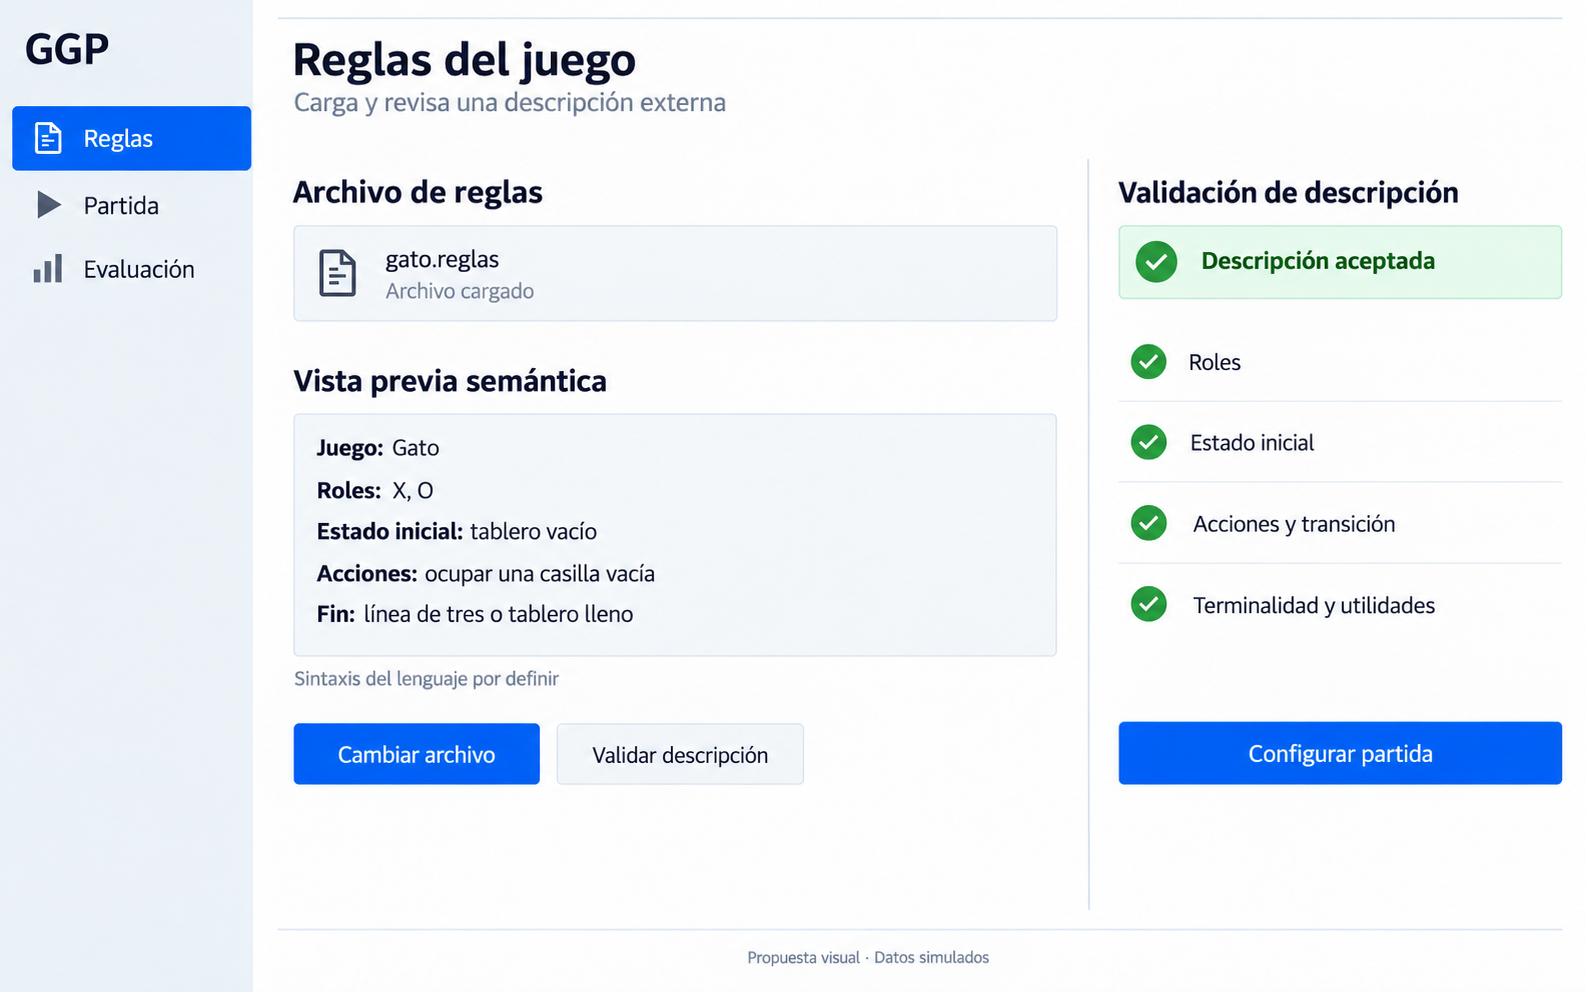
\includegraphics[width=\textwidth,height=0.80\textheight,keepaspectratio]{mockups/mockup_reglas.png}
    \caption{Prototipo aprobado de carga y revisión de una descripción externa de Gato. La validación y el contenido del archivo son ilustrativos; la sintaxis del lenguaje permanece por definir.}
    \label{fig:mockup-reglas}
\end{figure}

\paragraph{Partida de Gato.}
La Figura~\ref{fig:mockup-gato} propone una vista para una partida entre dos agentes. Presenta el tablero, el turno activo, las acciones legales, un historial y el espacio reservado para la siguiente decisión. Con ello separa la visualización de la partida de las consultas que el motor deberá resolver sobre legalidad y transición. La posición pausada y sus acciones se muestran solo como ejemplo de interacción, sin acreditar que se generen a partir de reglas ejecutables.

\begin{figure}[p]
    \centering
    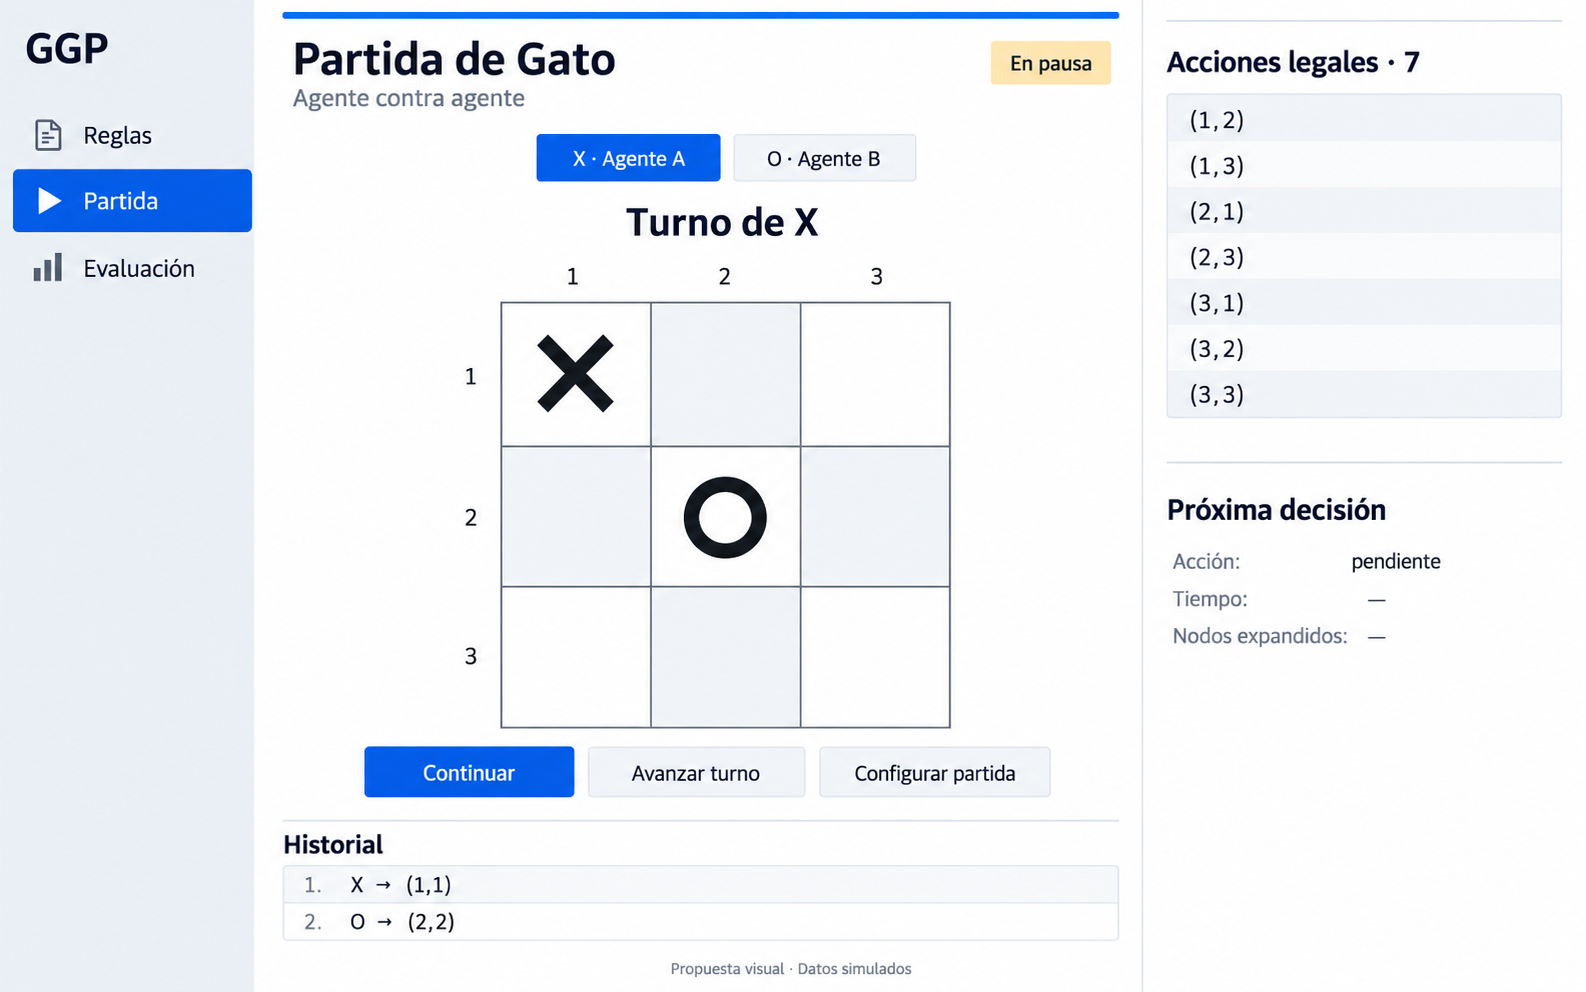
\includegraphics[width=\textwidth,height=0.80\textheight,keepaspectratio]{mockups/mockup_gato.png}
    \caption{Prototipo aprobado de una partida de Gato entre agentes. El tablero, historial, acciones legales y próxima decisión representan un estado ilustrativo.}
    \label{fig:mockup-gato}
\end{figure}

\paragraph{Partida de Ajedrez.}
La Figura~\ref{fig:mockup-ajedrez} reutiliza la misma organización para Ajedrez: tablero, turno, acciones legales, historial y próxima decisión. Su propósito es hacer visible que la interfaz no queda ligada a la geometría ni a las piezas de un único dominio; el cambio de juego corresponderá a la descripción externa y al modelo interno. La posición inicial y las veinte acciones mostradas son datos visuales de ejemplo, no una prueba de que el agente ya soporte las reglas completas de Ajedrez.

\begin{figure}[p]
    \centering
    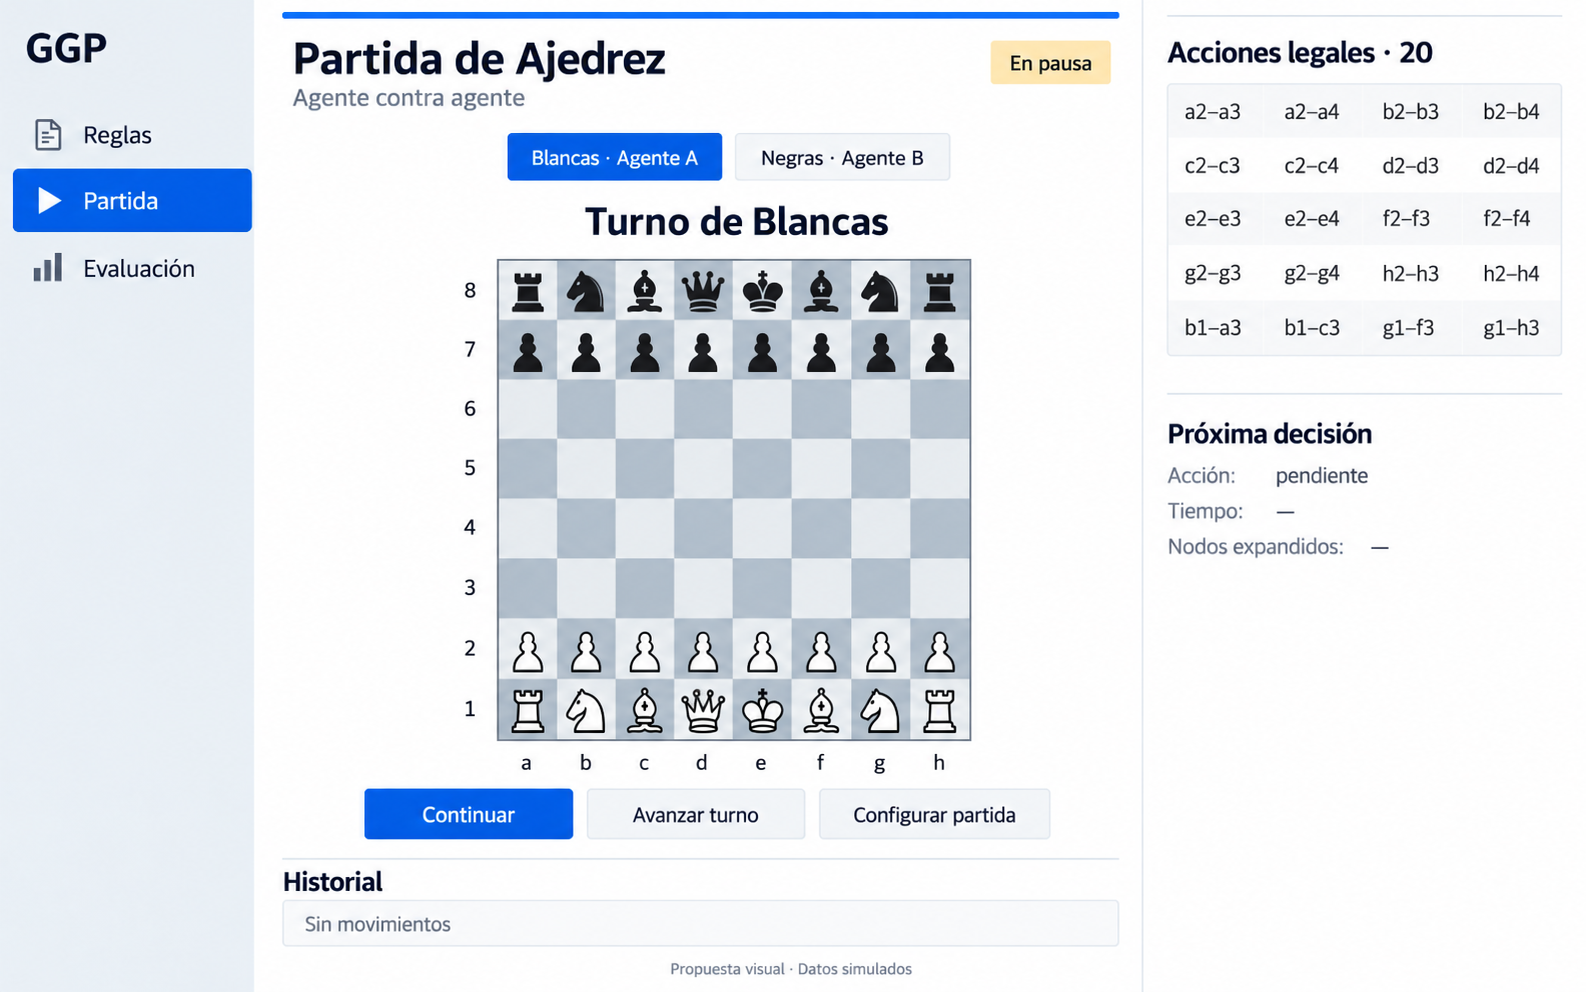
\includegraphics[width=\textwidth,height=0.80\textheight,keepaspectratio]{mockups/mockup_chess.png}
    \caption{Prototipo aprobado de una partida de Ajedrez entre agentes. La posición y las acciones son ilustrativas.}
    \label{fig:mockup-ajedrez}
\end{figure}

\paragraph{Preparación de la evaluación.}
La Figura~\ref{fig:mockup-evaluacion} representa la configuración previa de una comprobación de primera jugada en Ajedrez. Distingue el banco de casos, las condiciones de ejecución y el criterio de comparación, de acuerdo con la propuesta de métricas de la Sección~\ref{subsec:evaluacion_propuesta}. Las 30 posiciones, una ejecución por posición y el presupuesto de 1000 ms son valores de ejemplo; el tamaño definitivo del banco, las repeticiones, el presupuesto y el protocolo de Ajedrez continúan sujetos a acuerdo. La indicación de que las respuestas pertenecen al evaluador preserva la separación entre referencia independiente y agente evaluado.

\begin{figure}[p]
    \centering
    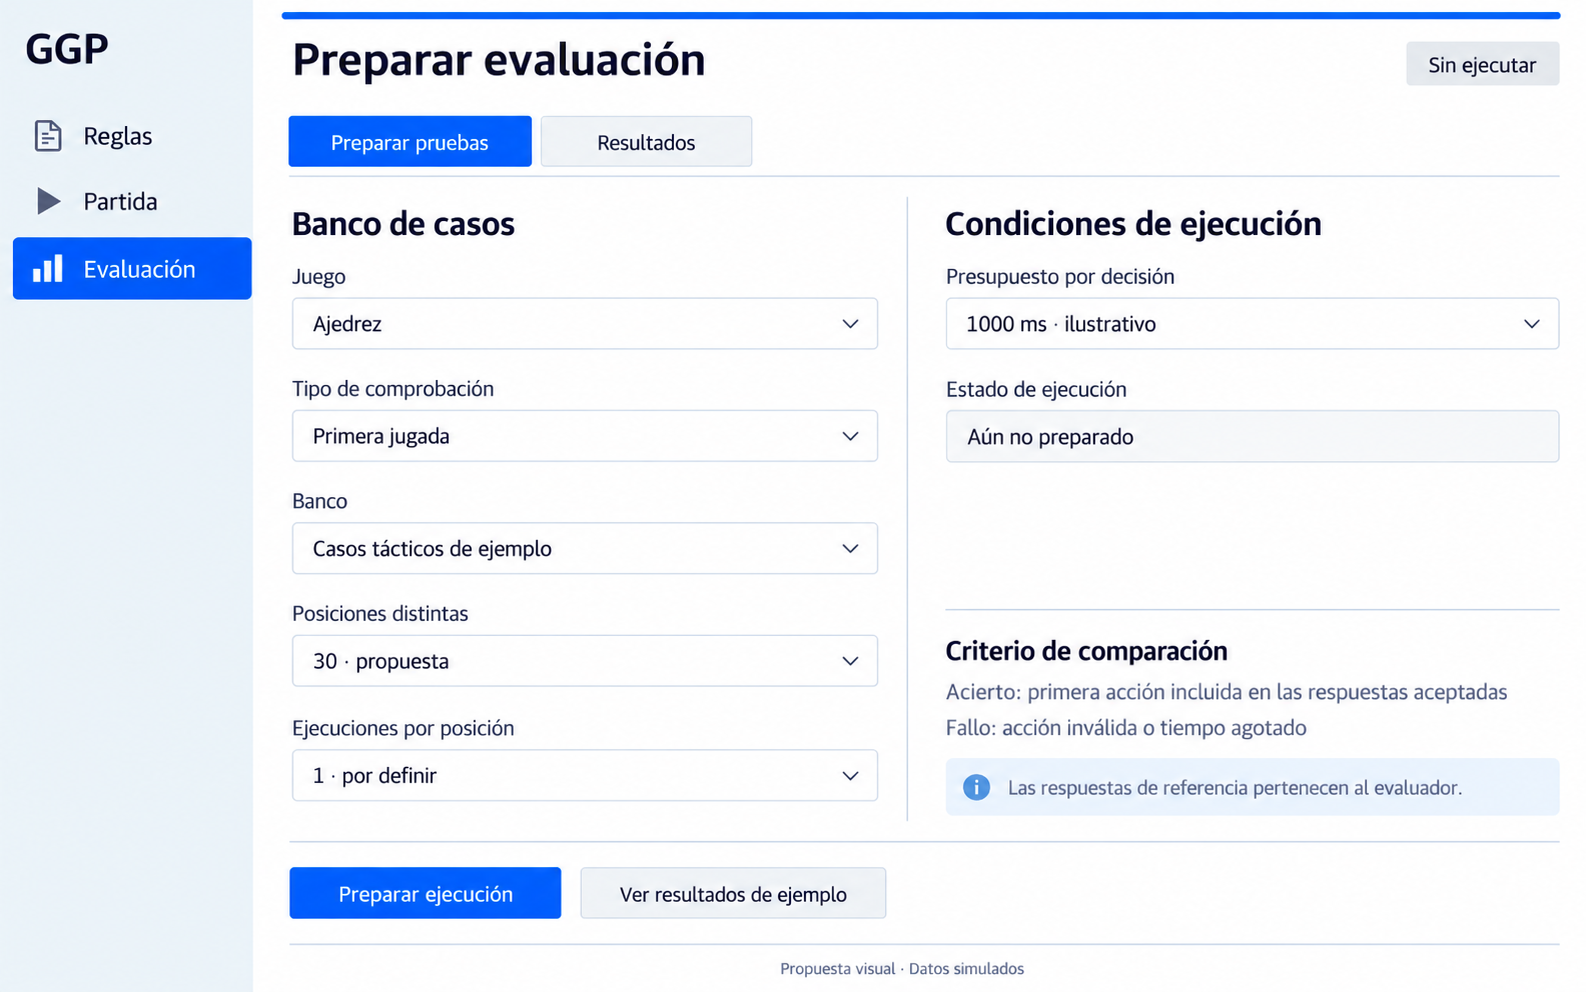
\includegraphics[width=\textwidth,height=0.80\textheight,keepaspectratio]{mockups/mockup_evaluacion.png}
    \caption{Prototipo aprobado de preparación de una evaluación táctica de primera jugada en Ajedrez. Las cantidades, el presupuesto y el estado de ejecución son ilustrativos y no describen un experimento realizado.}
    \label{fig:mockup-evaluacion}
\end{figure}

\paragraph{Resultados de evaluación.}
La Figura~\ref{fig:mockup-resultados} propone cómo reportar los indicadores definidos para la validación: acierto, tiempo por decisión, nodos expandidos, posiciones distintas, ejecuciones y detalle por caso. También conserva el motivo de terminación para que los tiempos agotados y otras incidencias permanezcan visibles en el registro. Los valores numéricos, los movimientos y el resumen de 4 de 5 casos son datos simulados; la figura no informa resultados experimentales ni selecciona un algoritmo de búsqueda.

\begin{figure}[p]
    \centering
    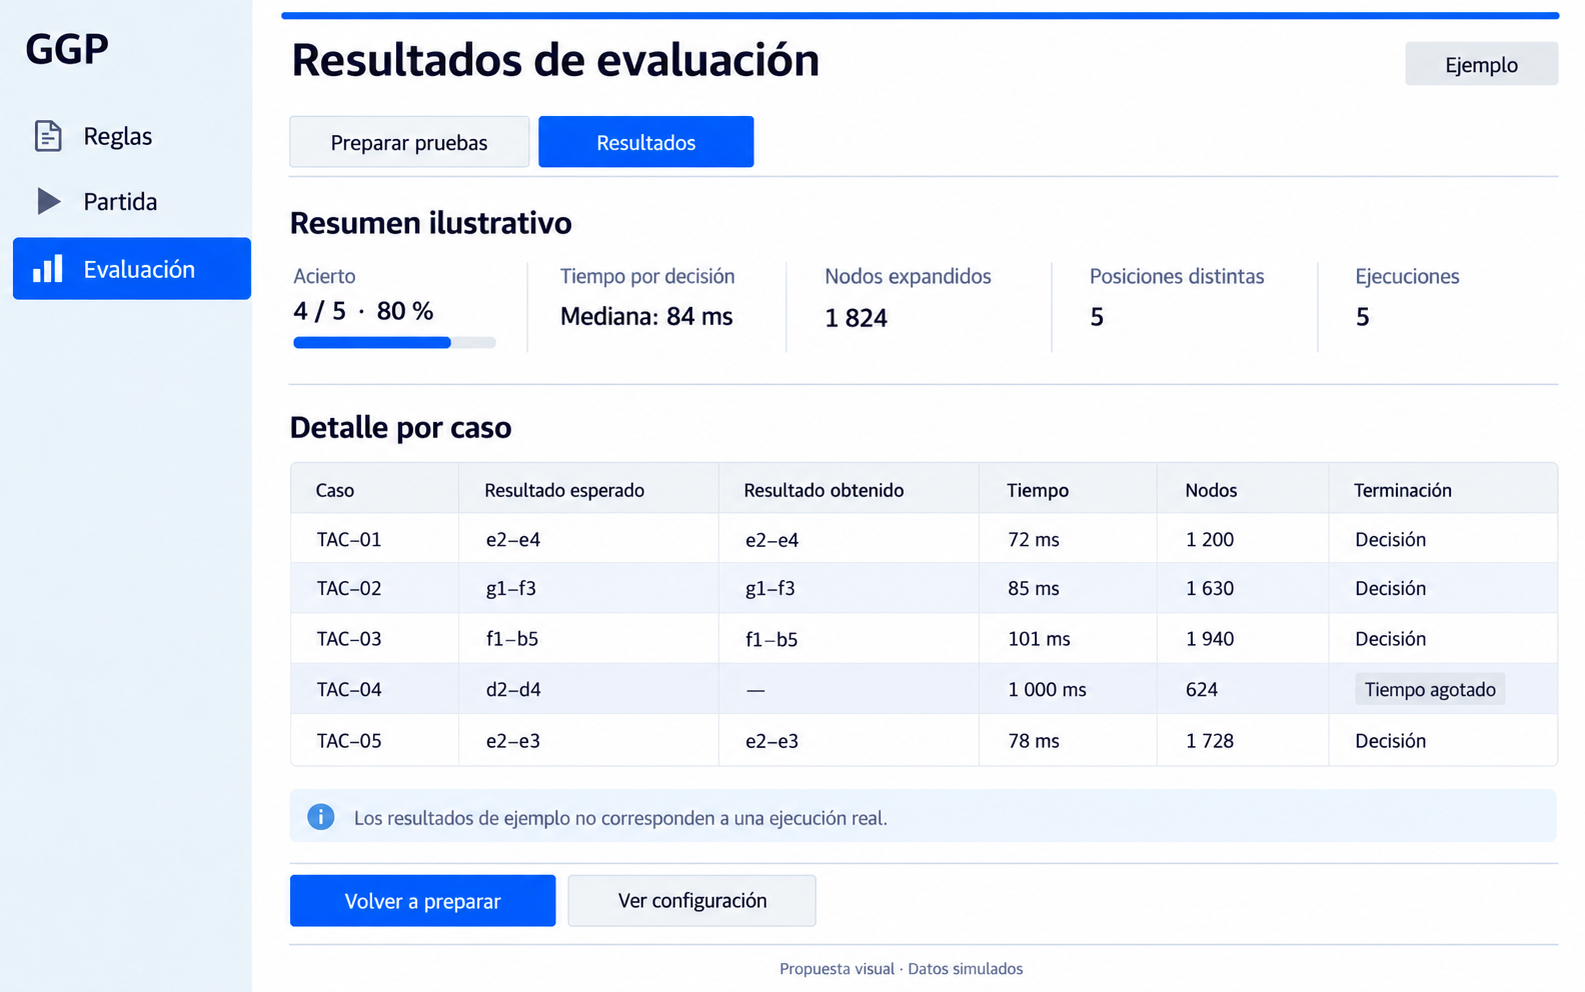
\includegraphics[width=\textwidth,height=0.80\textheight,keepaspectratio]{mockups/mockup_resultados.png}
    \caption{Prototipo aprobado del reporte de resultados de una evaluación. Las métricas y el detalle por caso muestran datos simulados, sin atribuir una ejecución real ni desempeño al agente.}
    \label{fig:mockup-resultados}
\end{figure}

\chapter{Desarrollo}






\chapter{Pruebas}



\chapter{Conclusiones y trabajo a futuro}


% ============================================================
%                        BIBLIOGRAFÍA
% ============================================================

\printbibliography[
    heading=bibintoc,
    title={Referencias}
]

% ============================================================
%                        BACKMATTER
% ============================================================

\backmatter

\chapter{Anexos}

\section{Cronogramas}

\newpage
\newpage
\null

\end{document}